\documentclass[compress,red]{beamer}
\mode<presentation>
\setbeamertemplate{navigation symbols}{}

\usepackage{pgfpages}
% \setbeameroption{show notes}
% \setbeameroption{show notes on second screen=right}

\usetheme{Warsaw}


%\hypersetup{pdfpagemode=FullScreen} % makes your presentation go automatically to full screen

% define your own colors:
\definecolor{Red}{rgb}{1,0,0}
\definecolor{Blue}{rgb}{0,0,1}
\definecolor{Green}{rgb}{0,1,0}
\definecolor{magenta}{rgb}{1,0,.6}
\definecolor{lightblue}{rgb}{0,.5,1}
\definecolor{lightpurple}{rgb}{.6,.4,1}
\definecolor{gold}{rgb}{.6,.5,0}
\definecolor{orange}{rgb}{1,0.4,0}
\definecolor{hotpink}{rgb}{1,0,0.5}
\definecolor{newcolor2}{rgb}{.5,.3,.5}
\definecolor{newcolor}{rgb}{0,.3,1}
\definecolor{newcolor3}{rgb}{1,0,.35}
\definecolor{darkgreen1}{rgb}{0, .35, 0}
\definecolor{darkgreen}{rgb}{0, .6, 0}
\definecolor{darkred}{rgb}{.75,0,0}

\xdefinecolor{olive}{cmyk}{0.64,0,0.95,0.4}
\xdefinecolor{purpleish}{cmyk}{0.75,0.75,0,0}


\useoutertheme[subsection=false]{smoothbars}


% include packages
\usepackage{subfigure}
\usepackage{multicol}
\usepackage{amsmath}
\usepackage{epsfig}
\usepackage{graphicx}
\usepackage[all,knot]{xy}

\xyoption{arc}
\usepackage{url}
\usepackage{multimedia}
\usepackage{hyperref}
\usepackage{helvet}
\usepackage[polish,english]{babel}
\usepackage[utf8]{inputenc}
\usepackage{multirow}

\newcommand{\backupbegin}{
   \newcounter{framenumberappendix}
   \setcounter{framenumberappendix}{\value{framenumber}}
}
\newcommand{\backupend}{
   \addtocounter{framenumberappendix}{-\value{framenumber}}
   \addtocounter{framenumber}{\value{framenumberappendix}} 
}

%%%%%%%%%%%%5
%\usepackage{geometry}
%\geometry{verbose,letterpaper}
%\usepackage{movie15}
%\usepackage{hyperref}
%%%%%%%

% greetings, introduce yourself


%  \includegraphics[height=5cm]{fig/WRlogo.ps}


\title[White Rabbit \hspace{2em}\insertframenumber/\inserttotalframenumber]
{White Rabbit}

\institute{
   \begin{center}
    Hardware and Timing Section  ~~~~~~~~~~~~~~~~~~~~~~~~ PERG ~~~~~~~~~~~~~~~~\\
    ~~~~Beam Controls Group~~~~~~~~~~~~ Institute of Electronic Systems \\
    ~~~~~~~~~~~~~~~~~~~~~CERN ~~~~~~~~~~~~~~~~~~~~~  Warsaw University of Technology \\
   \end{center}
}
\author{
Maciej Lipi\'{n}ski \\
% on behalf of Maciej Lipi\'{n}ski 
}
\date{Future Internet Engineering\\ Video/Tele-conference\\ 23rd November 2012}



\pgfdeclareimage[height=0.6cm]{wr-logo}{../../figures/logo/WRlogo.ps}
\logo{\pgfuseimage{wr-logo}}
\AtBeginSection[]

\begin{document}

\frame{\titlepage}
%%%%%%%%%%%%%%%%%%%%%%%%%%%%%%%%%%%%%%%%%%%%%%%%%%%%%%%%%%%%%%%%%%%%%%%%%%%%%%%%%%%%%%%%%%%%%%%%%%%%
\begin{frame}<beamer>{Outline}
    \tableofcontents %[currentsection]
\end{frame}



%%%%%%%%%%%%%%%%%%%%%%%%%%%%%%%%%%%%%%%%%%%%%%%%%%%%%%%%%%%%%%%%%%%%%%%%%%%%%%%%%%%%%%%%%%%%%%%%%%%%
\section{Introduction}
\subsection{}
%%%%%%%%%%%%%%%%%%%%%%%%%%%%%%%%%%%%%%%%%%%%%%%%%%%%%%%%%%%%%%%%%%%%%%%%%%%%%%%%%%%%%%%%%%%%%%%%%%%%
\begin{frame}{What is White Rabbit?}

\begin{columns}[c]
	\column{0.8\textwidth}
	  \begin{itemize}
		\item Accelerator's control and timing
		\item Based on well-known technologies
		\item Open Hardware and Open Software
		\item International collaboration
		\item Main features:
		\begin{itemize}
		  \item transparent,  {\bf high-accuracy} synchronization
		  \item low-latency,  {\bf deterministic} data delivery
		  \item designed for  {\bf high reliability}
		\end{itemize}
	  \end{itemize}
	\column{0.3\textwidth}
		\begin{center}
% 		\pause
		\hspace{-0.5cm}
		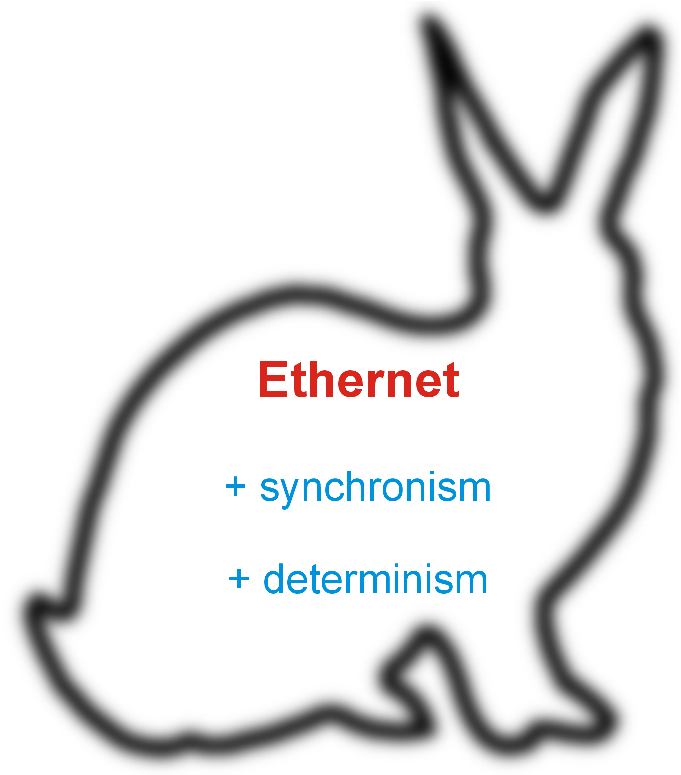
\includegraphics[width=1.1\textwidth]{../../figures/misc/rabbit.eps}
		\end{center}
	\end{columns}

\end{frame}
%%%%%%%%%%%%%%%%%%%%%%%%%%%%%%%%%%%%%%%%%%%%%%%%%%%%%%%%%%%%%%%%%%%%%%%%%%%%%%%%%%%%%%%%%%%%%%%%%%%%
%\section{White Rabbit~~~~}
\subsection{}
%%%%%%%%%%%%%%%%%%%%%%%%%%%%%%%%%%%%%%%%%%%%%%%%%%%%%%%%%%%%%%%%%%%%%%%%%%%%%%%%%%%%%%%%%%%%%%%%%%%%
\begin{frame}{White Rabbit -- enhanced Ethernet}

\begin{columns}[c]
  \column{.47\textwidth}
 

  \begin{itemize}
    \item Few thousands nodes
    \item Fiber medium
    \item Up to 10 km fiber links
    \item Bandwidth: 1 Gbps
    \item WR Switch: 18 ports
    \item Non-WR Devices
    \item Ethernet features (VLAN) \& protocols (SNMP)
  \end{itemize}

  \column{.6\textwidth}
    \begin{center}
    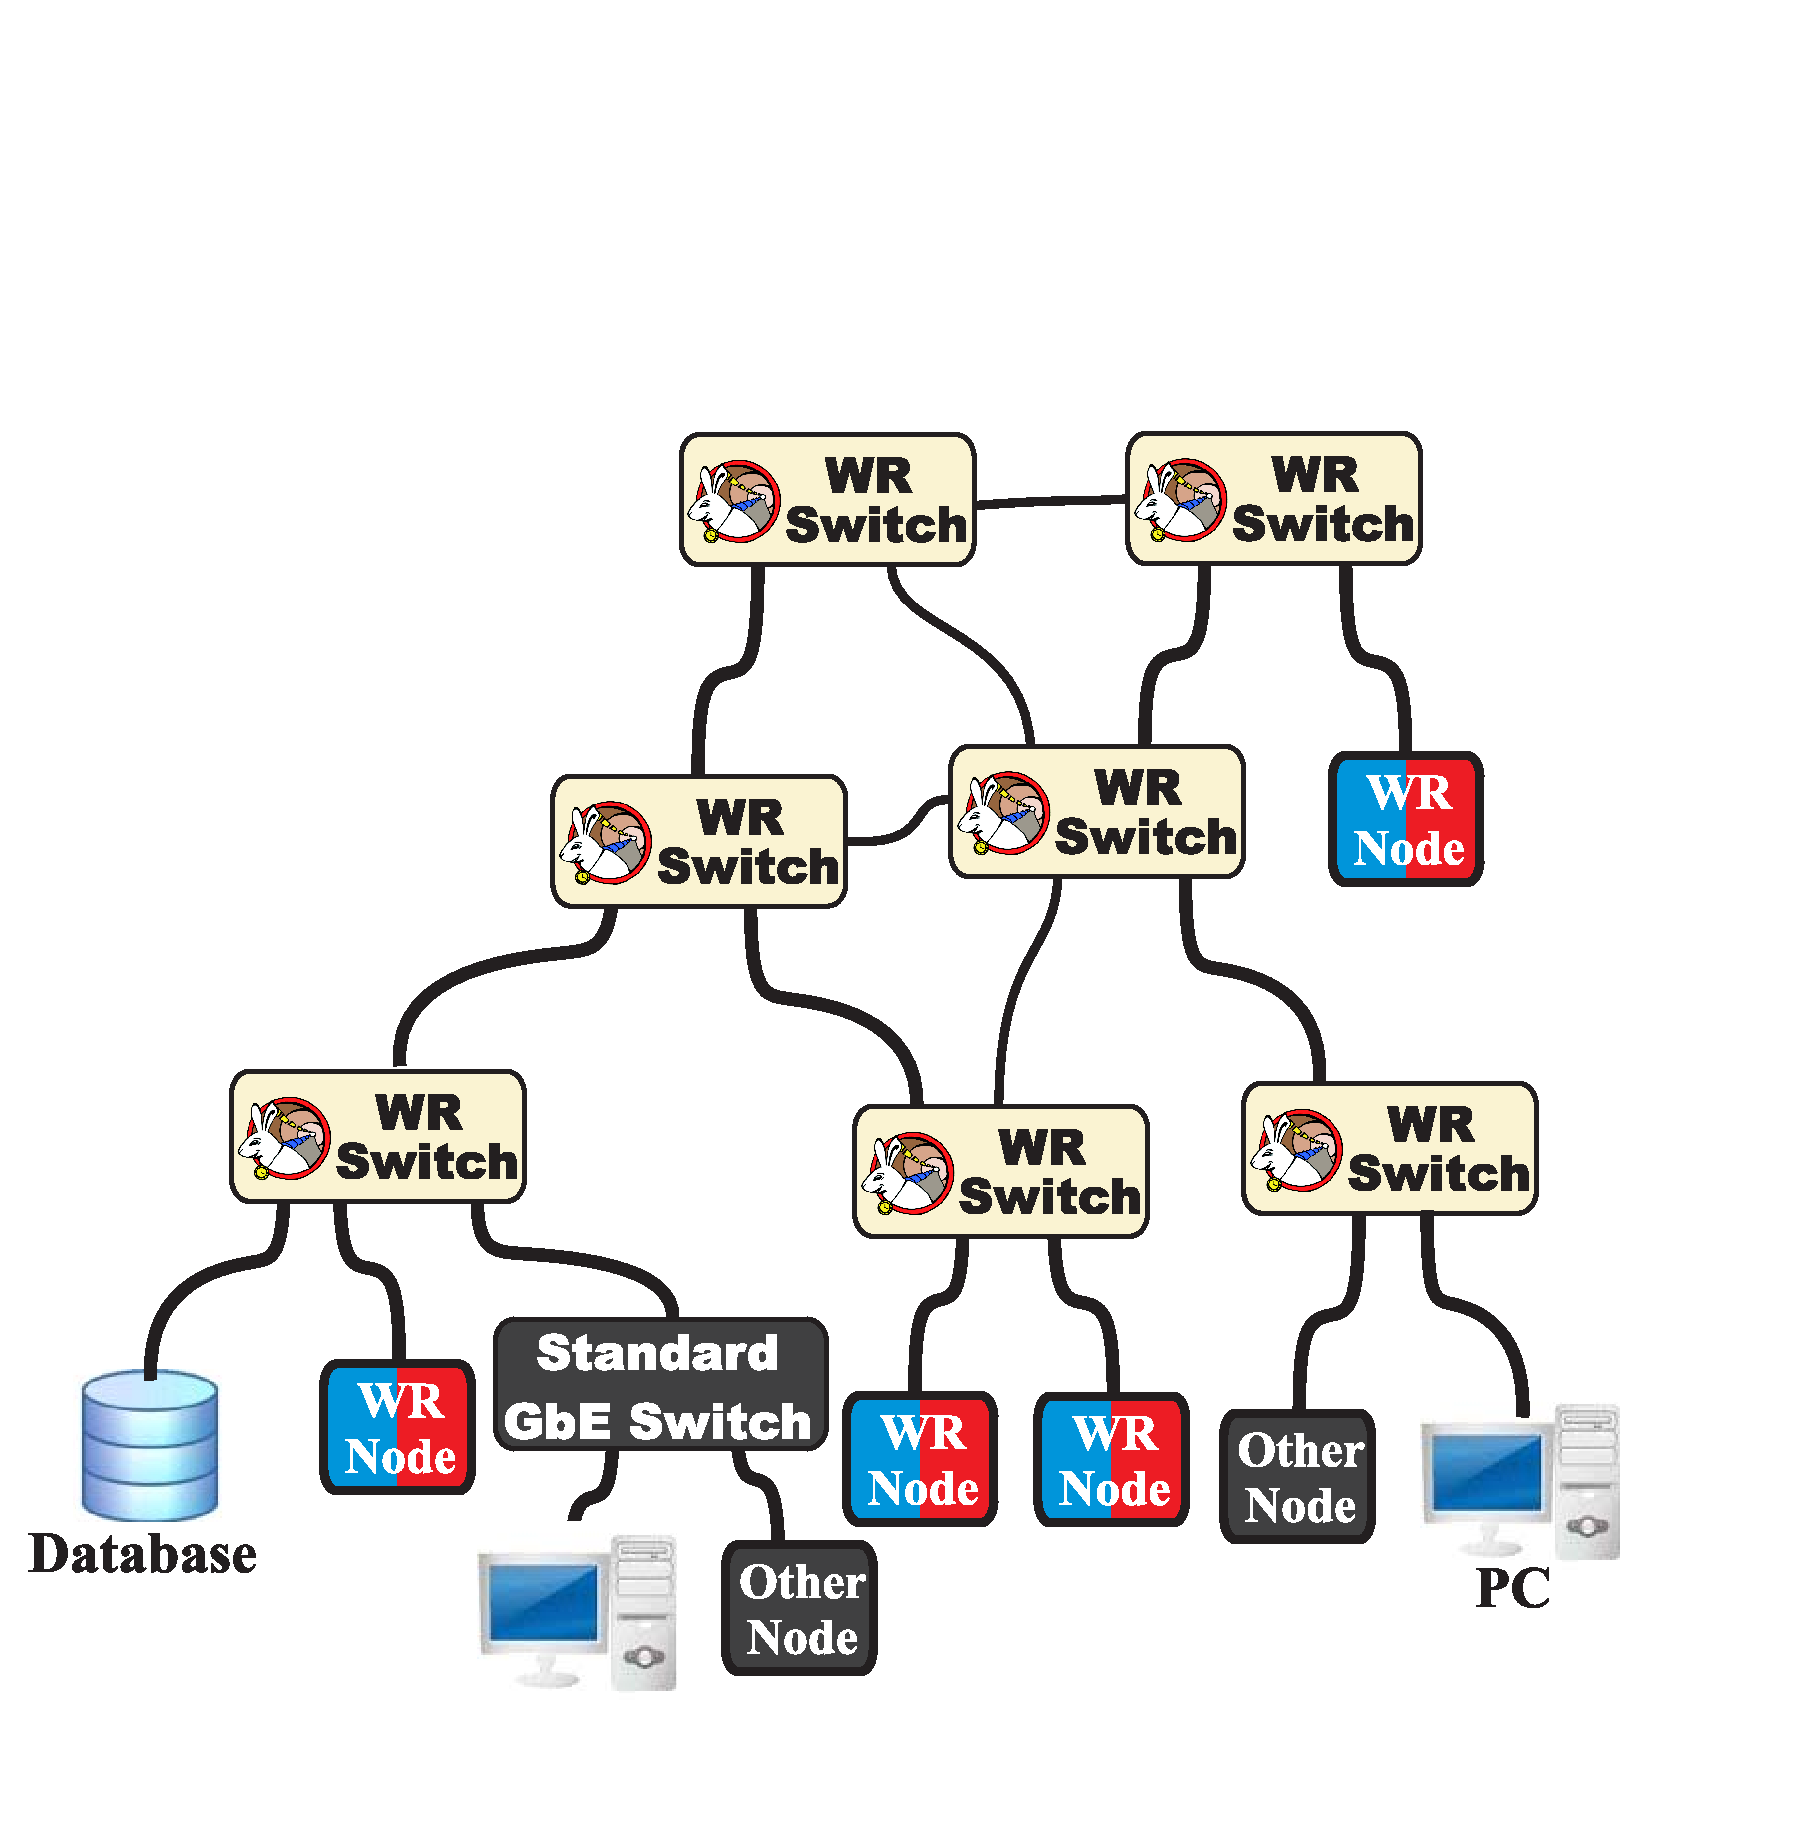
\includegraphics[width=1.0\textwidth]{../../figures/network/WR_network-ethernet.eps}
    \end{center}
\end{columns}

\end{frame}
%%%%%%%%%%%%%%%%%%%%%%%%%%%%%%%%%%%%%%%%%%%%%%%%%%%%%%%%%%%%%%%%%%%%%%%%%%%%%%%%%%%%%%%%%%%%%%%%%%%%
%\section{White Rabbit~~~~}
\subsection{}
%%%%%%%%%%%%%%%%%%%%%%%%%%%%%%%%%%%%%%%%%%%%%%%%%%%%%%%%%%%%%%%%%%%%%%%%%%%%%%%%%%%%%%%%%%%%%%%%%%%%
\begin{frame}{White Rabbit -- enhanced Ethernet}


\begin{columns}[c]
  \column{.47\textwidth}
 
  Two separate services (enhancements to Ethernet) provided by WR: 
  \begin{itemize}
    \item \color{blue!90}{High accuracy/precision synchronization}
    \item \color{red}{Deterministic, reliable and low-latency Control Data delivery}
  \end{itemize}

  \column{.6\textwidth}
    \begin{center}
    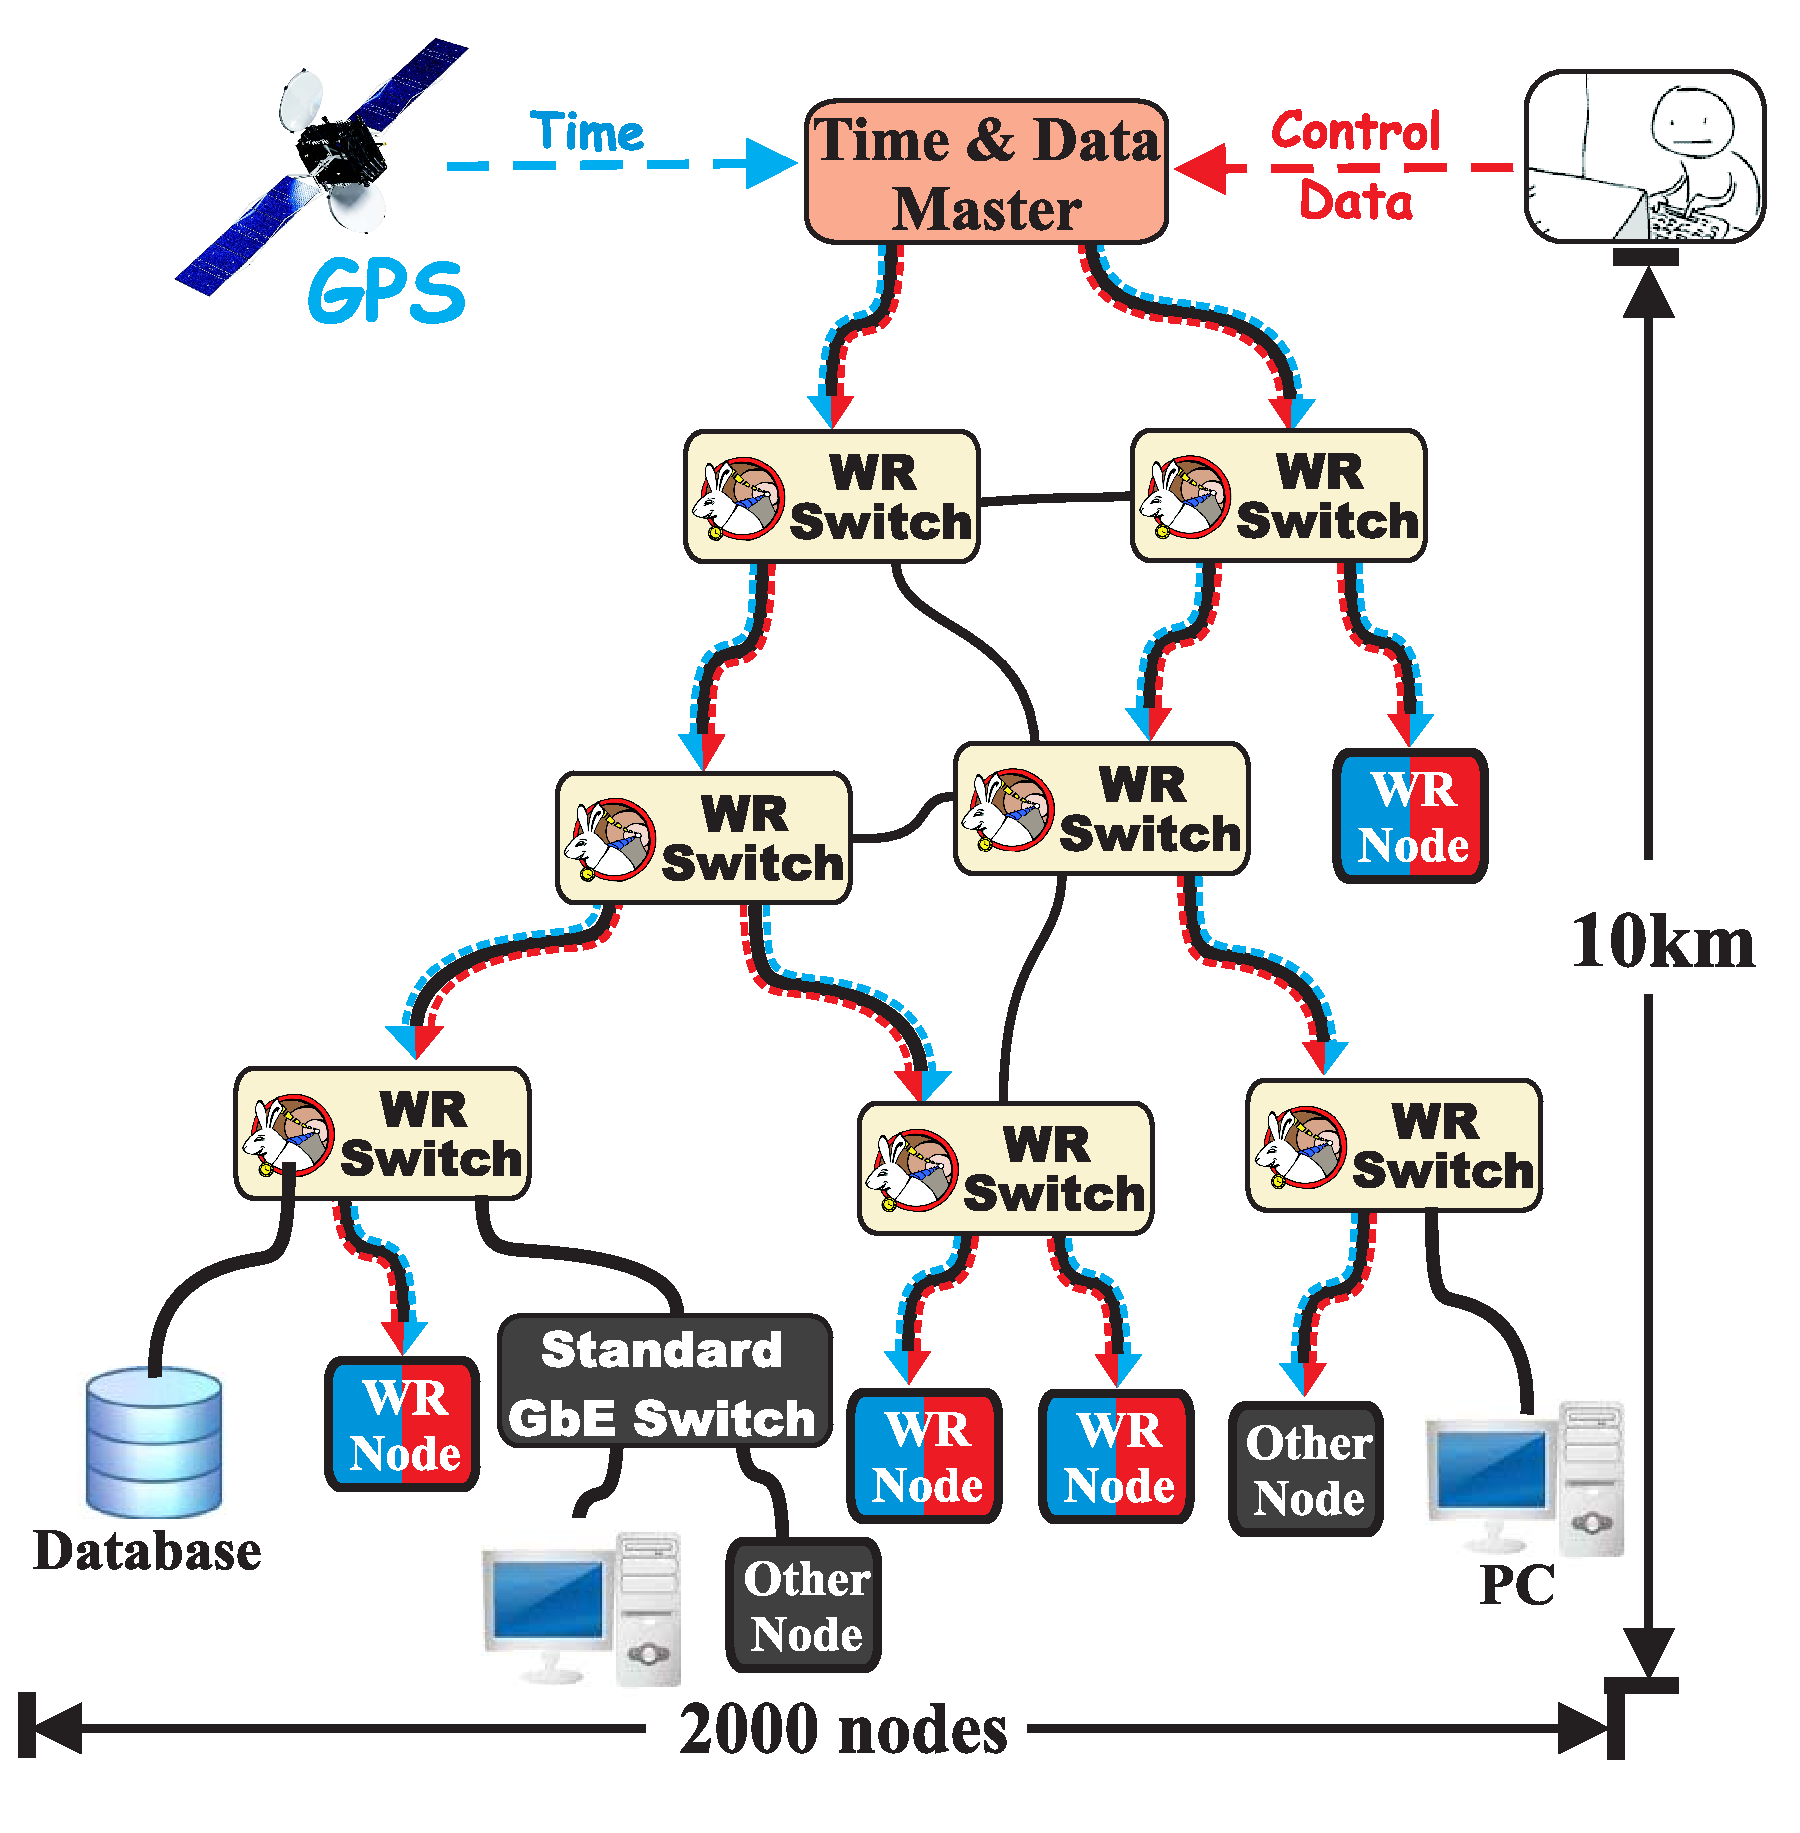
\includegraphics[width=1.0\textwidth]{../../figures/network/wr_network-enhanced.eps}
    \end{center}
\end{columns}

\end{frame}


% %%%%%%%%%%%%%%%%%%%%%%%%%%%%%%%%%%%%%%%%%%%%%%%%%%%%%%%%%%%%%%%%%%%%%%%%%%%%%%%%%%%%%%%%%%%%%%%%%%%%
% % \section{Motivation}
% \subsection{}
% %%%%%%%%%%%%%%%%%%%%%%%%%%%%%%%%%%%%%%%%%%%%%%%%%%%%%%%%%%%%%%%%%%%%%%%%%%%%%%%%%%%%%%%%%%%%%%%%%%%%
% \begin{frame}{Why White Rabbit ?}
% 
% \begin{columns}[c]
%   \column{0.55\textwidth}
% 
%     \begin{itemize}
% 	\item Renovation of CERN General Machine Timing (GMT)
% \small
% 	\item GMT is great but...:
% 	      \begin{itemize}
% 		  \item \textbf{RS-422}, 500kbps
% 		  \item \textbf{Unidirectional} communication
% 		  \item Separate network required
% 		  \item \textbf{Custom design, complicated maintenance}
% 	      \end{itemize}
% 	\item White Rabbit is meant to solve these problems
%     \end{itemize}
% 
%   \column{0.6\textwidth}
% 
%       \begin{center}
%       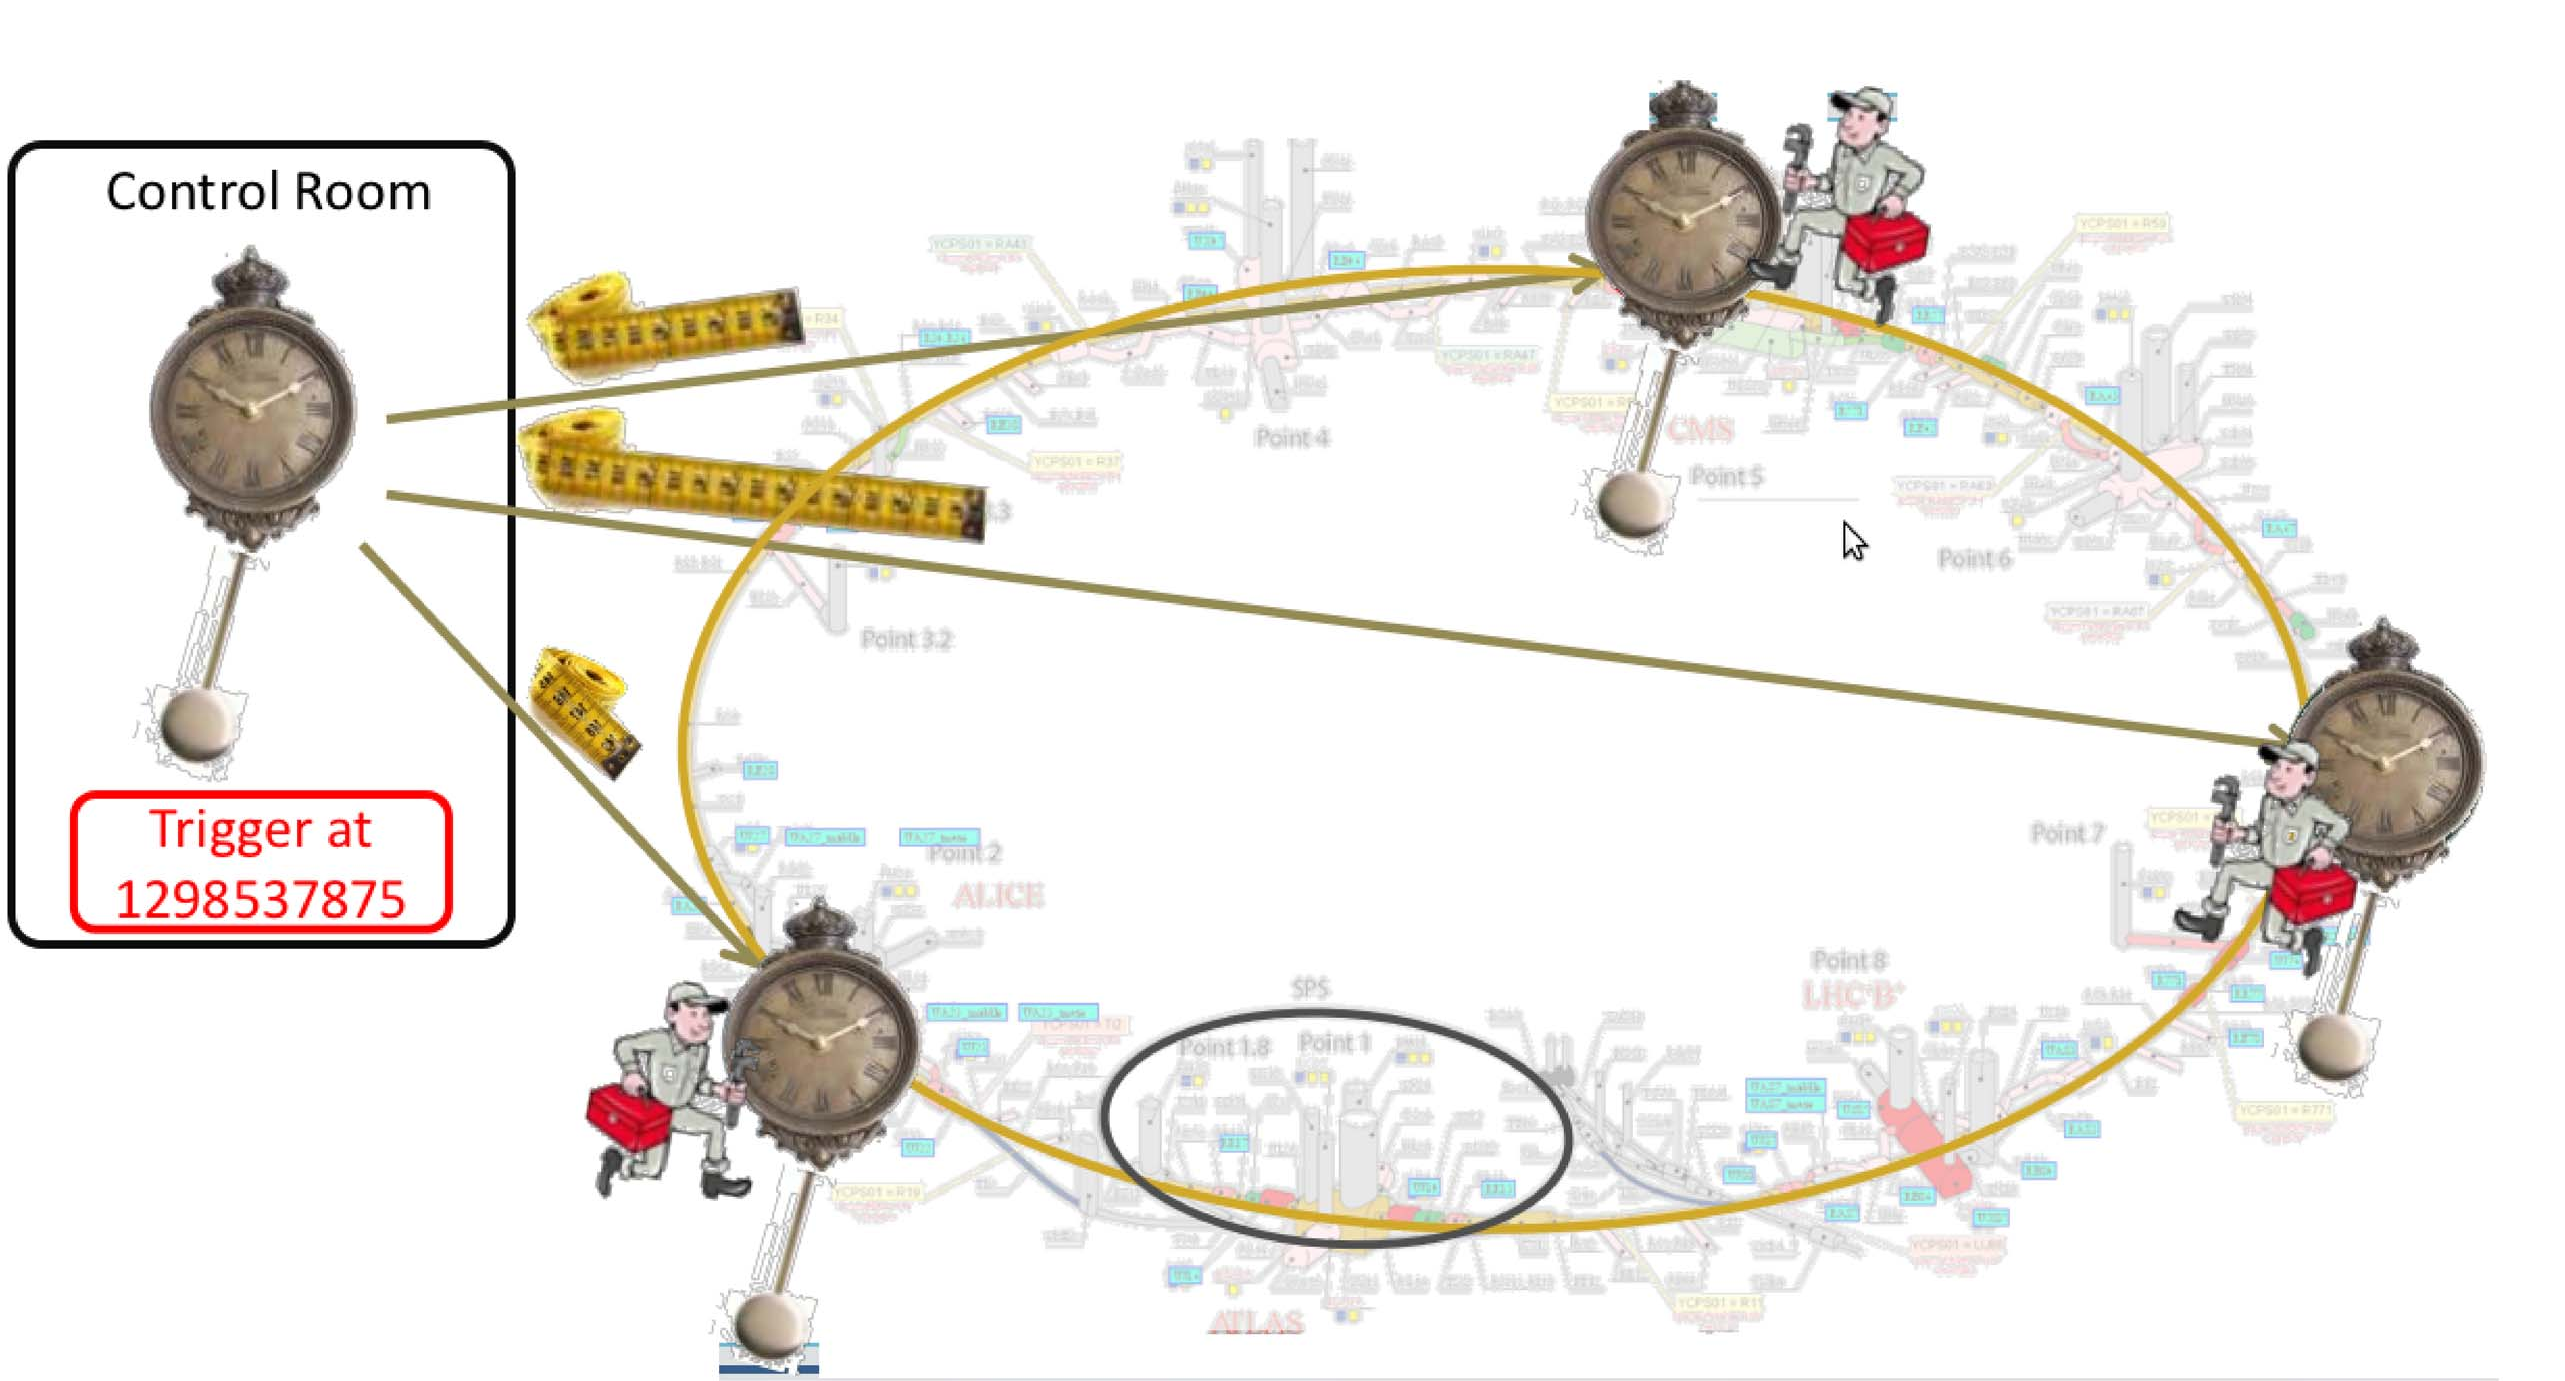
\includegraphics[width=1.0\textwidth]{../../figures/misc/GMT-2.eps} 
% %       \includegraphics<1>[width=1.0\textwidth]{../../figures/misc/GMT-1.eps} \pause
% %       \includegraphics<2>[width=1.0\textwidth]{../../figures/misc/GMT-2.eps} \pause
% %       \includegraphics<3>[width=1.0\textwidth]{../../figures/misc/GMT2WR.eps}
%       \end{center}
% 
% \end{columns}
% 
% \end{frame}

%%%%%%%%%%%%%%%%%%%%%%%%%%%%%%%%%%%%%%%%%%%%%%%%%%%%%%%%%%%%%%%%%%%%%%%%%%%%%%%%%%%%%%%%%%%%%%%%%%%%
\section{Time Distribution}
\subsection{}
%%%%%%%%%%%%%%%%%%%%%%%%%%%%%%%%%%%%%%%%%%%%%%%%%%%%%%%%%%%%%%%%%%%%%%%%%%%%%%%%%%%%%%%%%%%%%%%%%%%%
\begin{frame}{Time Distribution in White Rabbit Network}


\begin{columns}[c]
  \column{.47\textwidth}
 
  \begin{itemize}
    \item \textbf{\color{blue!90}{High accuracy/precision synchronization}}
    \item \color{gray}{Deterministic, reliable and low-latency Control Data delivery}
  \end{itemize}

  \column{.6\textwidth}
    \begin{center}
    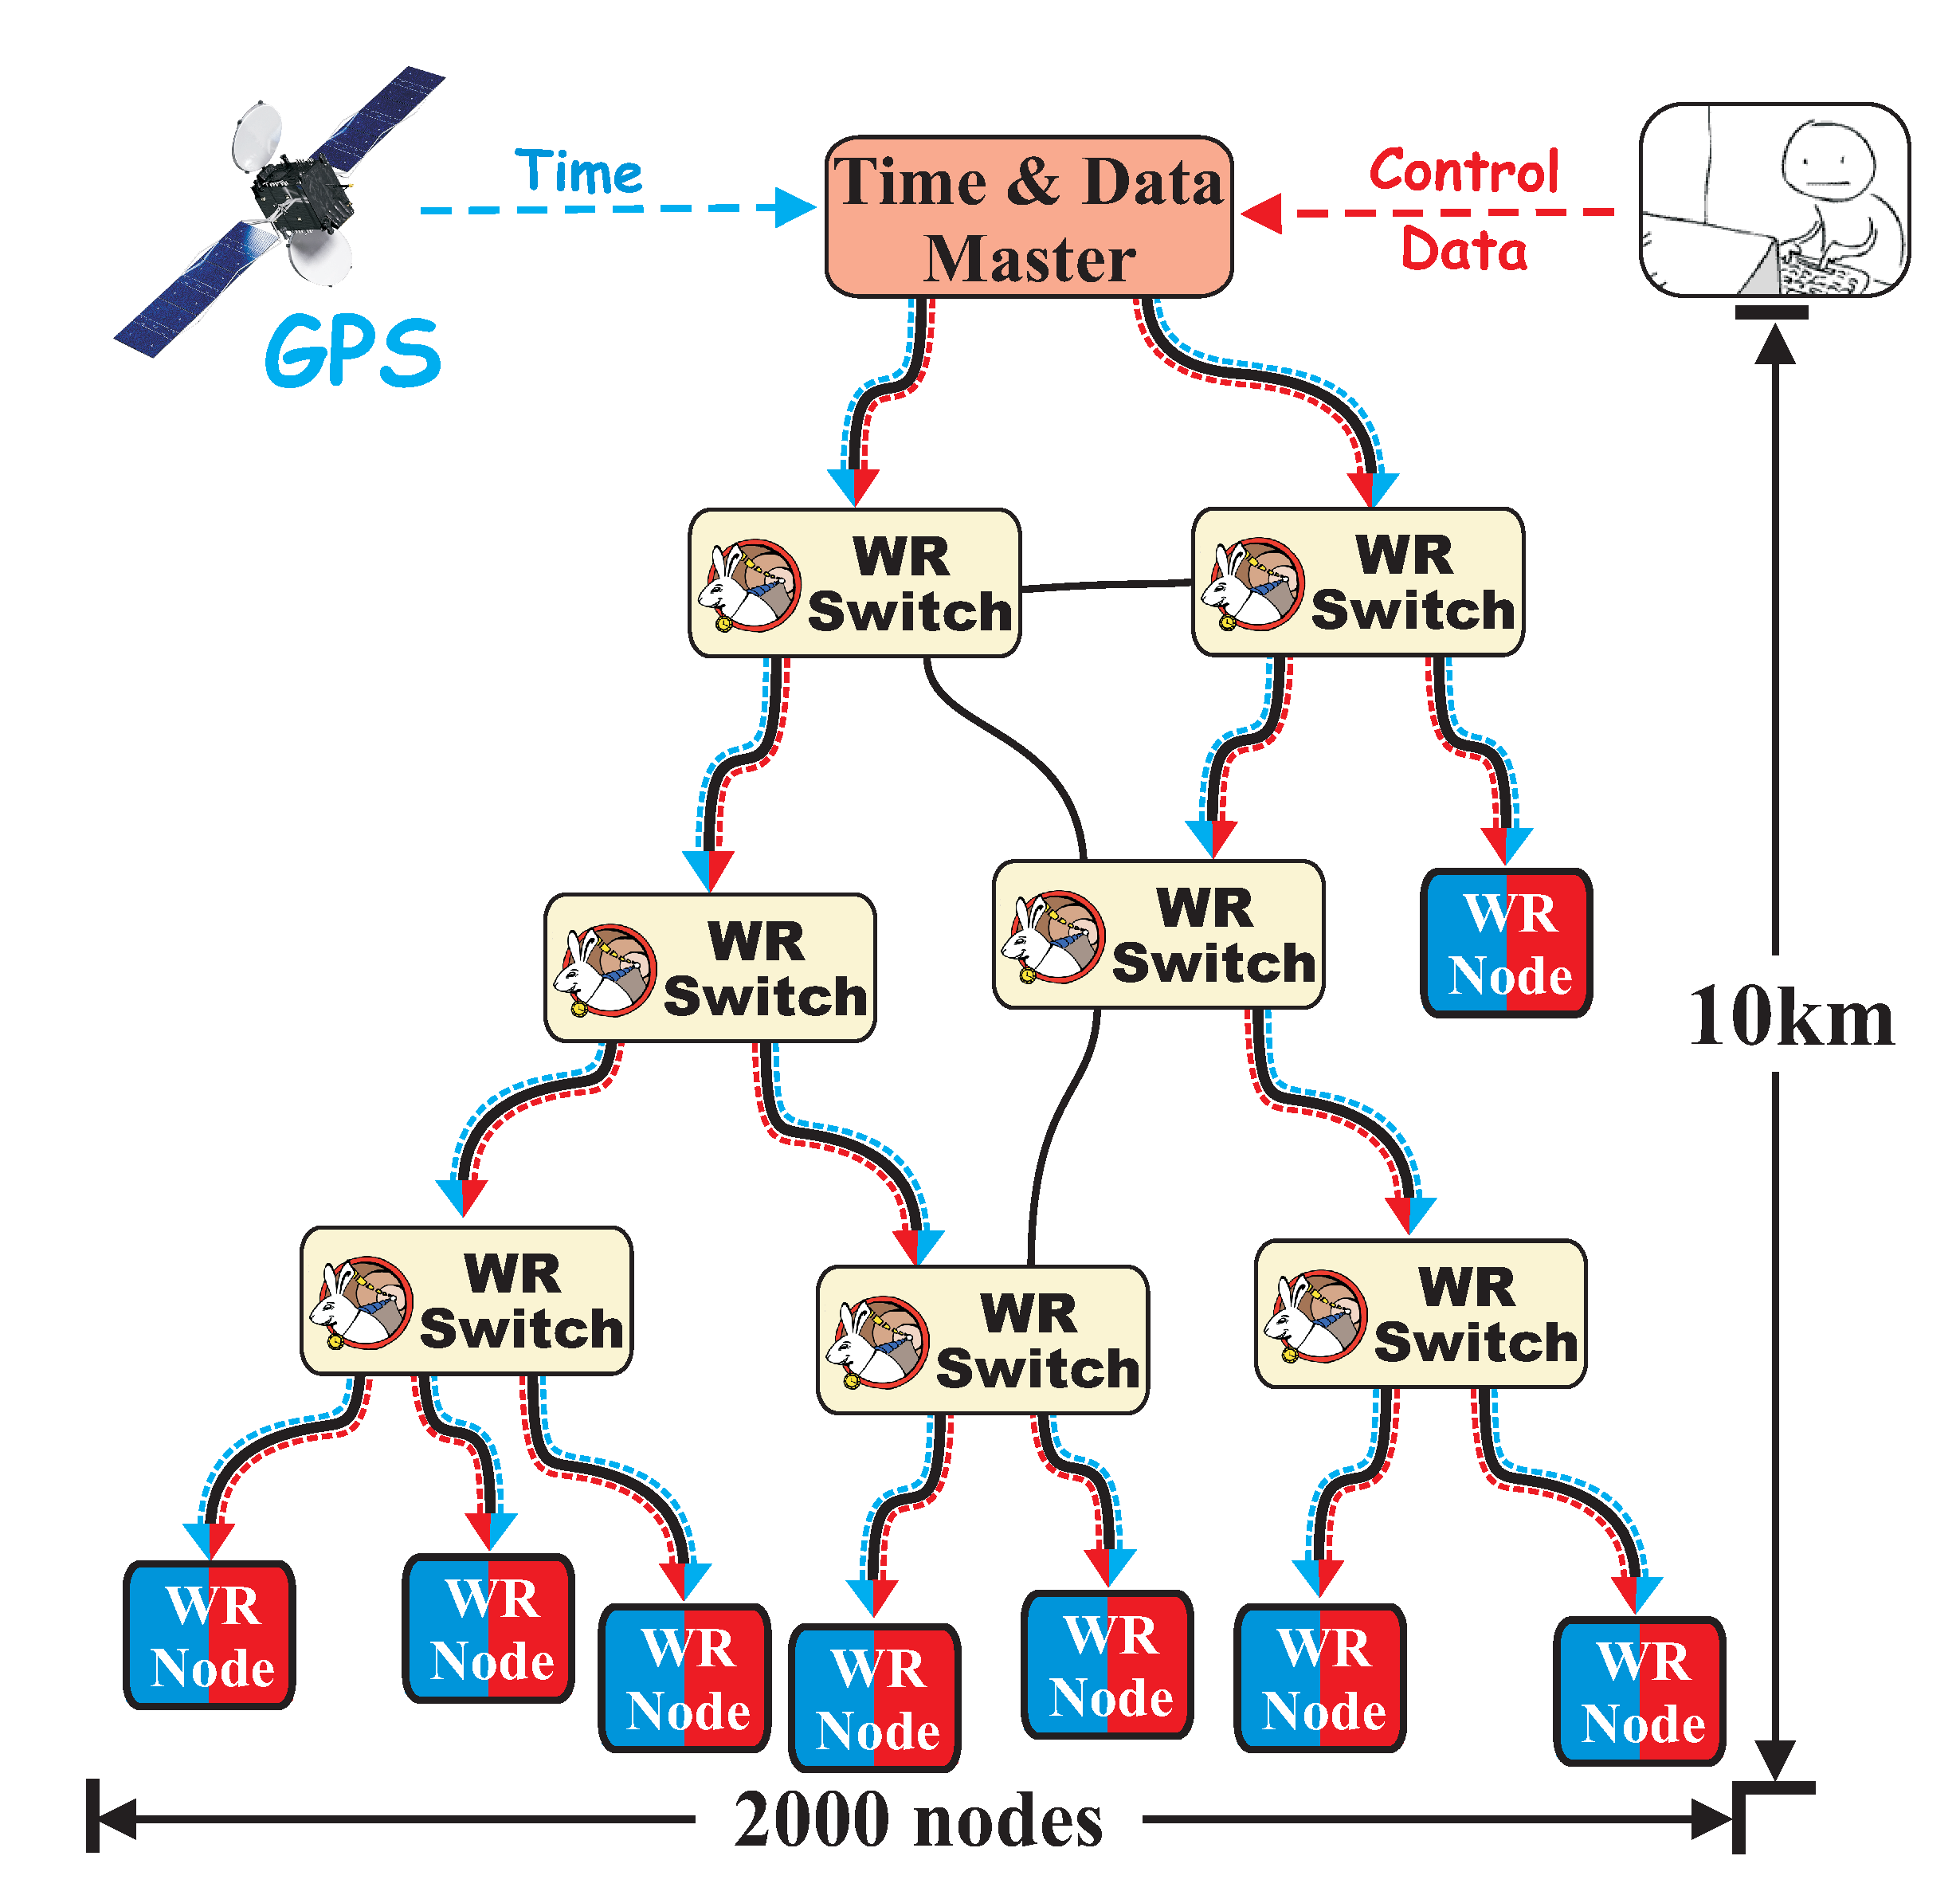
\includegraphics[height=1.0\textwidth]{../../figures/network/wr_network-new.ps}
    \end{center}
\end{columns}

\end{frame}
%%%%%%%%%%%%%%%%%%%%%%%%%%%%%%%%%%%%%%%%%%%%%%%%%%%%%%%%%%%%%%%%%%%%%%%%%%%%%%%%%%%%%%%%%%%%%%%%%%%%
% \section{}
% \subsection{}
%%%%%%%%%%%%%%%%%%%%%%%%%%%%%%%%%%%%%%%%%%%%%%%%%%%%%%%%%%%%%%%%%%%%%%%%%%%%%%%%%%%%%%%%%%%%%%%%%%%%
\begin{frame}{Time Distribution in White Rabbit Network}

  \begin{itemize}
    \item Synchronization with {\bf sub-ns} accuracy and {\bf ps} precision
    \item Combination of
	\begin{itemize}
	  \item Precision Time Protocol ({\bf PTP}) synchronization
	  \item Synchronous Ethernet ({\bf SyncE}) syntonization (L2)
	  \item Digital Dual-Mixer Time Difference ({\bf DDMTD}) phase detection
	\end{itemize}
  \end{itemize}
%     \begin{center}
%       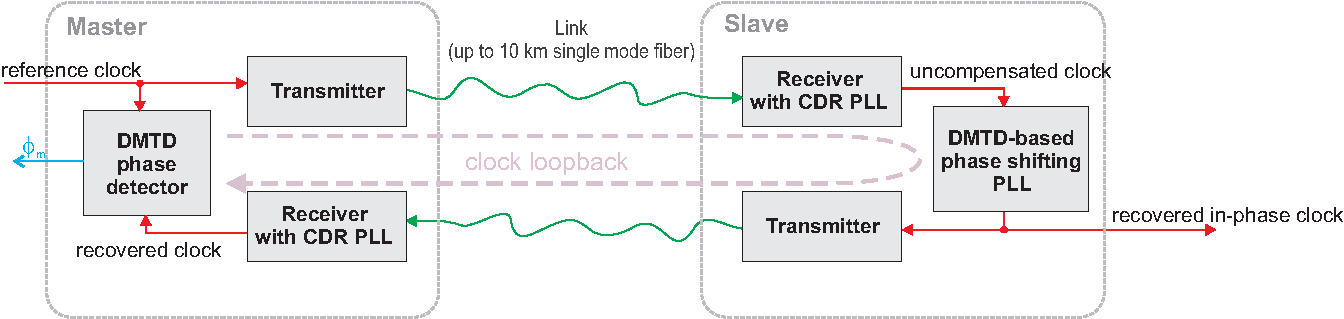
\includegraphics[width=1.0\textwidth]{fig/phase_tracking.eps}
%     \end{center}
\end{frame}
%%%%%%%%%%%%%%%%%%%%%%%%%%%%%%%%%%%%%%%%%%%%%%%%%%%%%%%%%%%%%%%%%%%%%%%%%%%%%%%%%%%%%%%%%%%%%%%%%%%%
% \section{}
% \subsection{}
%%%%%%%%%%%%%%%%%%%%%%%%%%%%%%%%%%%%%%%%%%%%%%%%%%%%%%%%%%%%%%%%%%%%%%%%%%%%%%%%%%%%%%%%%%%%%%%%%%%%
\begin{frame}{Precision Time Protocol (IEEE1588)}

\begin{columns}[c]
  \column{1.5in}
      \begin{center}
	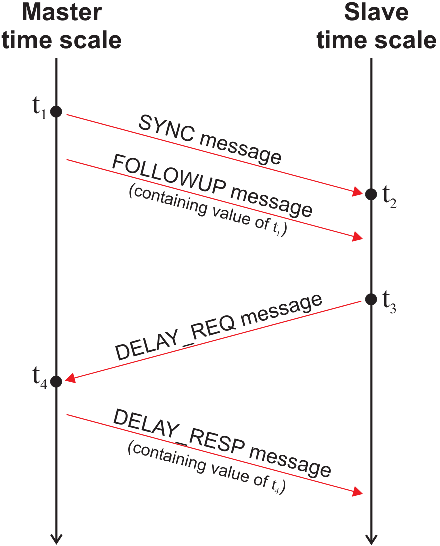
\includegraphics[height=5cm]{../../figures/protocol/ptp_exchange.eps}
      \end{center}
  \column{2.5in}
      \begin{itemize}
	  \item Packet-based synchronization protocol (mapping over UDP/IP, DeviceNet, and Ethernet)
	  \item Synchronizes local clock with the master clock
	  \item Link delay evaluated by measuring and exchanging packets tx/rx timestamps
      \end{itemize}
  \end{columns}

\end{frame}
%%%%%%%%%%%%%%%%%%%%%%%%%%%%%%%%%%%%%%%%%%%%%%%%%%%%%%%%%%%%%%%%%%%%%%%%%%%%%%%%%%%%%%%%%%%%%%%%%%%%
% \subsection{}
%%%%%%%%%%%%%%%%%%%%%%%%%%%%%%%%%%%%%%%%%%%%%%%%%%%%%%%%%%%%%%%%%%%%%%%%%%%%%%%%%%%%%%%%%%%%%%%%%%%%
% %\begin{frame}{Addressing the issues}
% \begin{frame}{PTP is OK but ...}
% 
%   \resizebox{11cm}{!} 
%   {
%     \begin{tabular}{ r c l }
%   {\bf What are the issues...} 	& {\bf and}      & {\bf ... how we address them}  \\
% 				&     		 &        \\
%       PTP-base		 	& \multirow{2}{*}{$\Rightarrow$}  & \multirow{2}{*}{SyncE }\\
%       syntonization	        &      		 &        \\
% 				&      		 &        			\\
%       limited             	&\multirow{2}{*}{$\Rightarrow$}  	 & SyncE \\
%       precision and resolution  &      		 & DDTMD phase detection\\
% 				&    		 &        \\
% 			        &      		 & SyncE  \\
%       unknown link asymmetry    & $\Rightarrow$  & DDTMD phase detection \\
% 				&      		 & WR Link Delay Model \\
% 				&      		 &        \\
%       \multicolumn{3}{c}{WR extension to PTP ({\bf WRPTP}) for } \\
%       \multicolumn{3}{c}{extra data exchange and logic} \\
%     \end{tabular}
%   }
% \end{frame}
%%%%%%%%%%%%%%%%%%%%%%%%%%%%%%%%%%%%%%%%%%%%%%%%%%%%%%%%%%%%%%%%%%%%%%%%%%%%%%%%%%%%%%%%%%%%%%%%%%%%
% \section{}
% \subsection{}
%%%%%%%%%%%%%%%%%%%%%%%%%%%%%%%%%%%%%%%%%%%%%%%%%%%%%%%%%%%%%%%%%%%%%%%%%%%%%%%%%%%%%%%%%%%%%%%%%%%%
\setbeamertemplate{background}{\includegraphics[width=0.95\paperwidth]{figs/syncE.v2.eps}} 
\begin{frame}{Synchronous Ethernet (SyncE)}

\begin{columns}[c]
\column{0.11\textwidth}
\column{0.99\textwidth}
    \begin{itemize}    
      \item All network devices use the same physical layer clock
      \item Clock is encoded in the Ethernet carrier and recovered by the receiver chip (PHY).
    \end{itemize}
    \vspace{6.7cm}
\end{columns}

\end{frame}
\setbeamertemplate{background}{} 
%%%%%%%%%%%%%%%%%%%%%%%%%%%%%%%%%%%%%%%%%%%%%%%%%%%%%%%%%%%%%%%%%%%%%%%%%%%%%%%%%%%%%%%%%%%%%%%%%%%%
% \section{}
% \subsection{}
%%%%%%%%%%%%%%%%%%%%%%%%%%%%%%%%%%%%%%%%%%%%%%%%%%%%%%%%%%%%%%%%%%%%%%%%%%%%%%%%%%%%%%%%%%%%%%%%%%%%
\setbeamertemplate{background}{\includegraphics[width=0.95\paperwidth]{figs/ddmtd.v2.eps}} 
\begin{frame}{DDMTD: Phase Tracking}

\begin{columns}[c]
\column{0.01\textwidth}
\column{0.99\textwidth}
    \begin{itemize}
      \item PTP limitation: timestamping granularity
      \item Solution: take advantage of SyncE and measure phase shift
    \end{itemize}
    \vspace{3.9cm}
\end{columns}
\end{frame}
\setbeamertemplate{background}{} 
%%%%%%%%%%%%%%%%%%%%%%%%%%%%%%%%%%%%%%%%%%%%%%%%%%%%%%%%%%%%%%%%%%%%%%%%%%%%%%%%%%%%%%%%%%%%%%%%%%%%
% \section{White Rabbit PTP}
% \subsection{}
% %%%%%%%%%%%%%%%%%%%%%%%%%%%%%%%%%%%%%%%%%%%%%%%%%%%%%%%%%%%%%%%%%%%%%%%%%%%%%%%%%%%%%%%%%%%%%%%%%%%%
\begin{frame}{PTP is OK but ...}

  \resizebox{11cm}{!} 
  {
    \begin{tabular}{ r c l }
  {\bf What are the issues...} 	& {\bf and}      & {\bf ... how we address them}  \\
				&     		 &        \\
      PTP-base		 	& \multirow{2}{*}{$\Rightarrow$}  & \multirow{2}{*}{SyncE }\\
      syntonization	        &      		 &        \\
				&      		 &        			\\
      limited             	&\multirow{2}{*}{$\Rightarrow$}  	 & SyncE \\
      precision and resolution  &      		 & DDTMD phase detection\\
				&    		 &        \\
			        &      		 & SyncE  \\
      unknown link asymmetry    & $\Rightarrow$  & DDTMD phase detection \\
				&      		 & WR Link Delay Model \\
				&      		 &        \\
      \multicolumn{3}{c}{WR extension to PTP ({\bf WR PTP}) for } \\
      \multicolumn{3}{c}{extra data exchange and logic} \\
    \end{tabular}
  }
\end{frame}
%%%%%%%%%%%%%%%%%%%%%%%%%%%%%%%%%%%%%%%%%%%%%%%%%%%%%%%%%%%%%%%%%%%%%%%%%%%%%%%%%%%%%%%%%%%%%%%%%%%%
% \subsection{}
%%%%%%%%%%%%%%%%%%%%%%%%%%%%%%%%%%%%%%%%%%%%%%%%%%%%%%%%%%%%%%%%%%%%%%%%%%%%%%%%%%%%%%%%%%%%%%%%%%%%
% \begin{frame}{WR Link Delay Model}
% 
%   \begin{center}
%   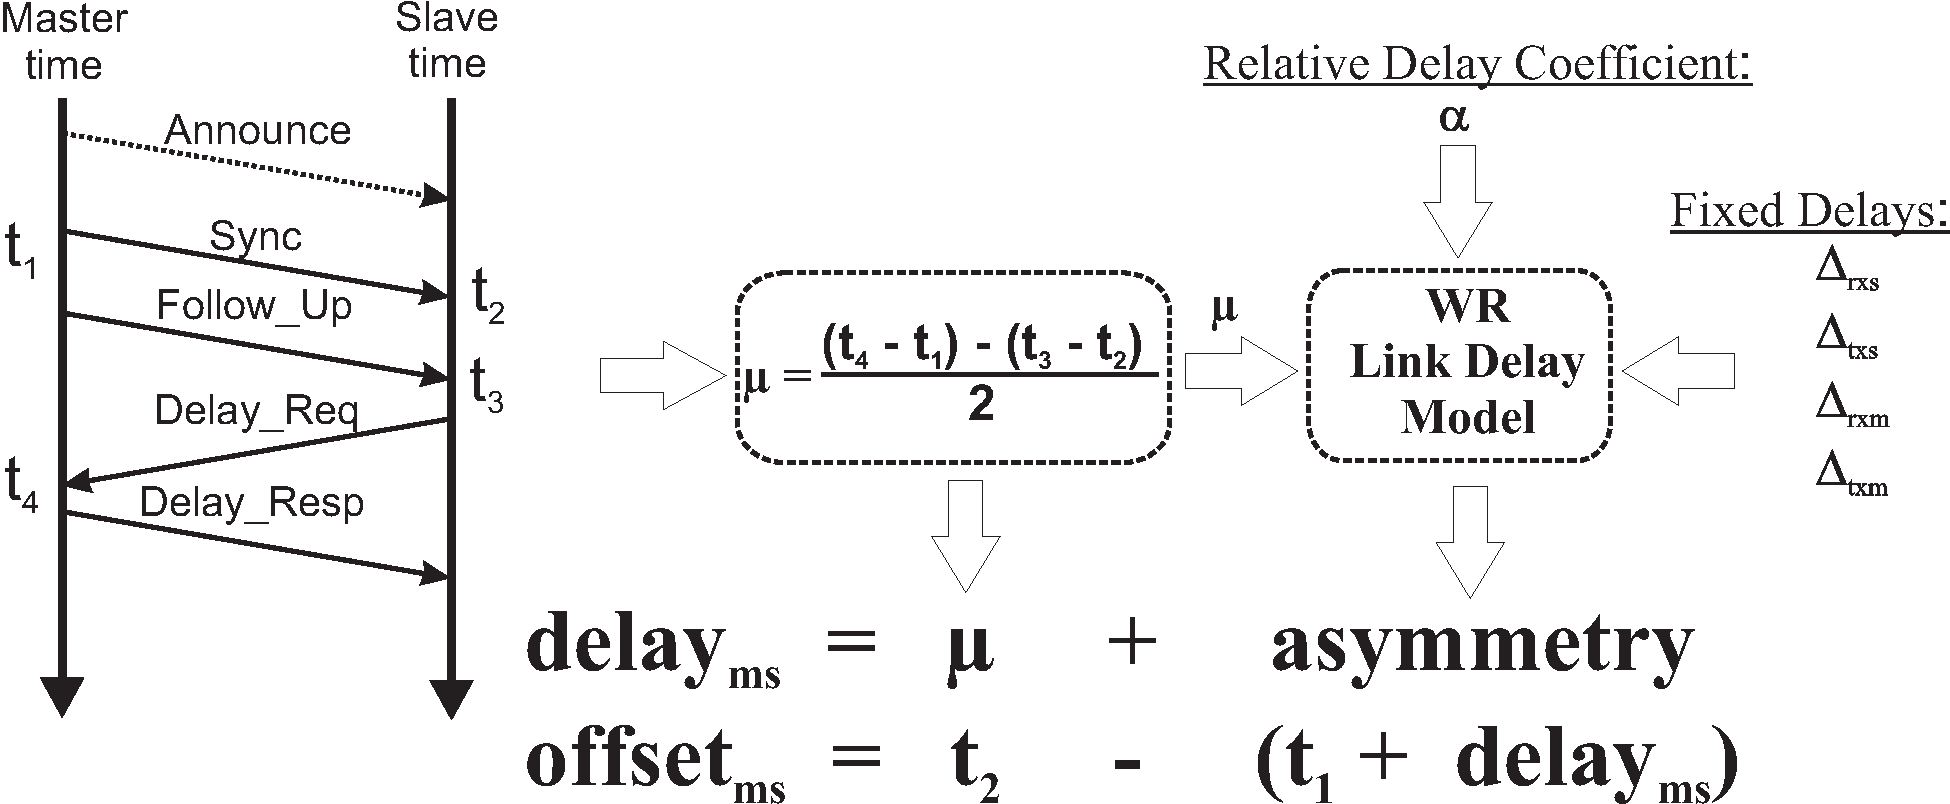
\includegraphics[height=4cm]{../../figures/protocol/wrLinkModel.eps}
%   \end{center}
% 
%   \begin{columns}[c]
%   \column{1.5in}
% 
%     \begin{center}
%       \textbf{Solution for Ethernet over a Single-mode Optical Fiber}
%     \end{center}    
% 
%   \column{2.7in}
% 
%     \begin{equation}
%       \nonumber asymmetry = \Delta_{tx_m} + \Delta_{rx_s} - \frac{\Delta - \alpha \mu + \alpha \Delta}{2 + \alpha}
%     \end{equation}
% 
%   \end{columns}
% 
% \end{frame}
%%%%%%%%%%%%%%%%%%%%%%%%%%%%%%%%%%%%%%%%%%%%%%%%%%%%%%%%%%%%%%%%%%%%%%%%%%%%%%%%%%%%%%%%%%%%%%%%%%%%
% \section{}
% \subsection{}
%%%%%%%%%%%%%%%%%%%%%%%%%%%%%%%%%%%%%%%%%%%%%%%%%%%%%%%%%%%%%%%%%%%%%%%%%%%%%%%%%%%%%%%%%%%%%%%%%%%%
\begin{frame}{WR PTP}

  \begin{itemize}
    \item Extension to PTP (IEEE1588) -- defined as PTP Profile
    \item Addresses PTP's limitations \\(granularity, asymmetry, syntonization)
    \item Compatible with "standard" PTP gear
%     \item Ongoing standardization effort
    \item Lab \& field-tested for sub-ns synchronization
  \end{itemize}
%   \pause
  \begin{block}{According to ISPCS Plug Fest results ...}
    \begin{center}
      \textbf{... White Rabbit is the most accurate PTP implementation in the world!}
     \end{center}
  \end{block}

\end{frame}
%%%%%%%%%%%%%%%%%%%%%%%%%%%%%%%%%%%%%%%%%%%%%%%%%%%%%%%%%%%%%%%%%%%%%%%%%%%%%%%%%%%%%%%%%%%%%%%%%%%%
%\section{Status}
%\subsection{}
%%%%%%%%%%%%%%%%%%%%%%%%%%%%%%%%%%%%%%%%%%%%%%%%%%%%%%%%%%%%%%%%%%%%%%%%%%%%%%%%%%%%%%%%%%%%%%%%%%%%
\begin{frame}{WR PTP Standardization Effort}

\begin{columns}[c]
\column{0.65\textwidth}
  \begin{itemize}
    \item \textbf{We want to standardize WR PTP}
    \item Many possibilities 
    \begin{itemize}
      \item Profile (ITU-T, IEEE, ...)
      \item AVB gen 2
      \item Consortium
    \end{itemize}
    \item WR Standardization Group
    \begin{itemize}
      \item John Eidson
      \item ITU-T/IEEE people
      \item Companies 
    \end{itemize}
    \item ISPCS2012: 
    \begin{itemize}
      \item PTP will be openned for revision
      \item WR PTP proposed to be included in PTPv3
    \end{itemize}
    \item \textbf{Standardization goal: include WR into PTPv3}
  \end{itemize}

\column{0.4\textwidth}
    \begin{center}
      \textbf{John Eidson:} \\
      \textit{“Why don't you propose to include WR into PTPv3 ? You could do it in that way...”}
     \end{center}

\end{columns}



% \begin{columns}[c]
% \column{0.65\textwidth}
%   \begin{itemize}
%     \item<1-> \textbf{We want to standardize WR PTP}
%     \item<2-> Many possibilities 
%     \begin{itemize}
%       \item Profile (ITU-T, IEEE, ...)
%       \item AVB gen 2
%       \item Consortium
%     \end{itemize}
%     \item<3-> WR Standardization Group
%     \begin{itemize}
%       \item John Eidson
%       \item ITU-T/IEEE people
%       \item Companies 
%     \end{itemize}
%     \item<5-> ISPCS2012: 
%     \begin{itemize}
%       \item PTP will be openned for revision
%       \item WR PTP proposed to be included in PTPv3
%     \end{itemize}
%   \end{itemize}
% 
% \column{0.4\textwidth}
%     \begin{center}
%       \textcolor<1-3>{white}{\textbf<4->{John Eidson:} }\\
%       \textcolor<1-3>{white}{\textit<4->{“Why don't you propose to include WR into PTPv3 ? You could do it in that way...”}}
%      \end{center}
% 
% \end{columns}
% 
\end{frame}

%%%%%%%%%%%%%%%%%%%%%%%%%%%%%%%%%%%%%%%%%%%%%%%%%%%%%%%%%%%%%%%%%%%%%%%%%%%%%%%%%%%%%%%%%%%%%%%%%%%%
%\section{Status}
%\subsection{}
% %%%%%%%%%%%%%%%%%%%%%%%%%%%%%%%%%%%%%%%%%%%%%%%%%%%%%%%%%%%%%%%%%%%%%%%%%%%%%%%%%%%%%%%%%%%%%%%%%%%%
% \begin{frame}{WR PTP Standardization effort}
% 
% \begin{columns}[c]
% \column{0.2\textwidth}
% 
% \column{0.6\textwidth}
% 
%   \begin{block}{~~~~~~~Standardization goal}
%     \begin{center}
%       \textbf{WR PTP included into PTPv3}
%      \end{center}
%   \end{block}
% 
% \column{0.2\textwidth}
% 
% \end{columns}
% % \pause
%     \begin{center}
%     \includegraphics[width=0.5\textwidth]{figs/wrSupport.eps}
%     \end{center}
% 
% \end{frame}


%%%%%%%%%%%%%%%%%%%%%%%%%%%%%%%%%%%%%%%%%%%%%%%%%%%%%%%%%%%%%%%%%%%%%%%%%%%%%%%%%%%%%%%%%%%%%%%%%%%%
\section{Data Distribution}
\subsection{}
%%%%%%%%%%%%%%%%%%%%%%%%%%%%%%%%%%%%%%%%%%%%%%%%%%%%%%%%%%%%%%%%%%%%%%%%%%%%%%%%%%%%%%%%%%%%%%%%%%%%
\begin{frame}{Data distribution in White Rabbit}


\begin{columns}[c]
  \column{.47\textwidth}
 
  \begin{itemize}
    \item \color{gray}{High accuracy/precision synchronization}
    \item \textbf{\color{red}{Deterministic, reliable and low-latency Control Data delivery}}
  \end{itemize}

  \column{.6\textwidth}
    \begin{center}
    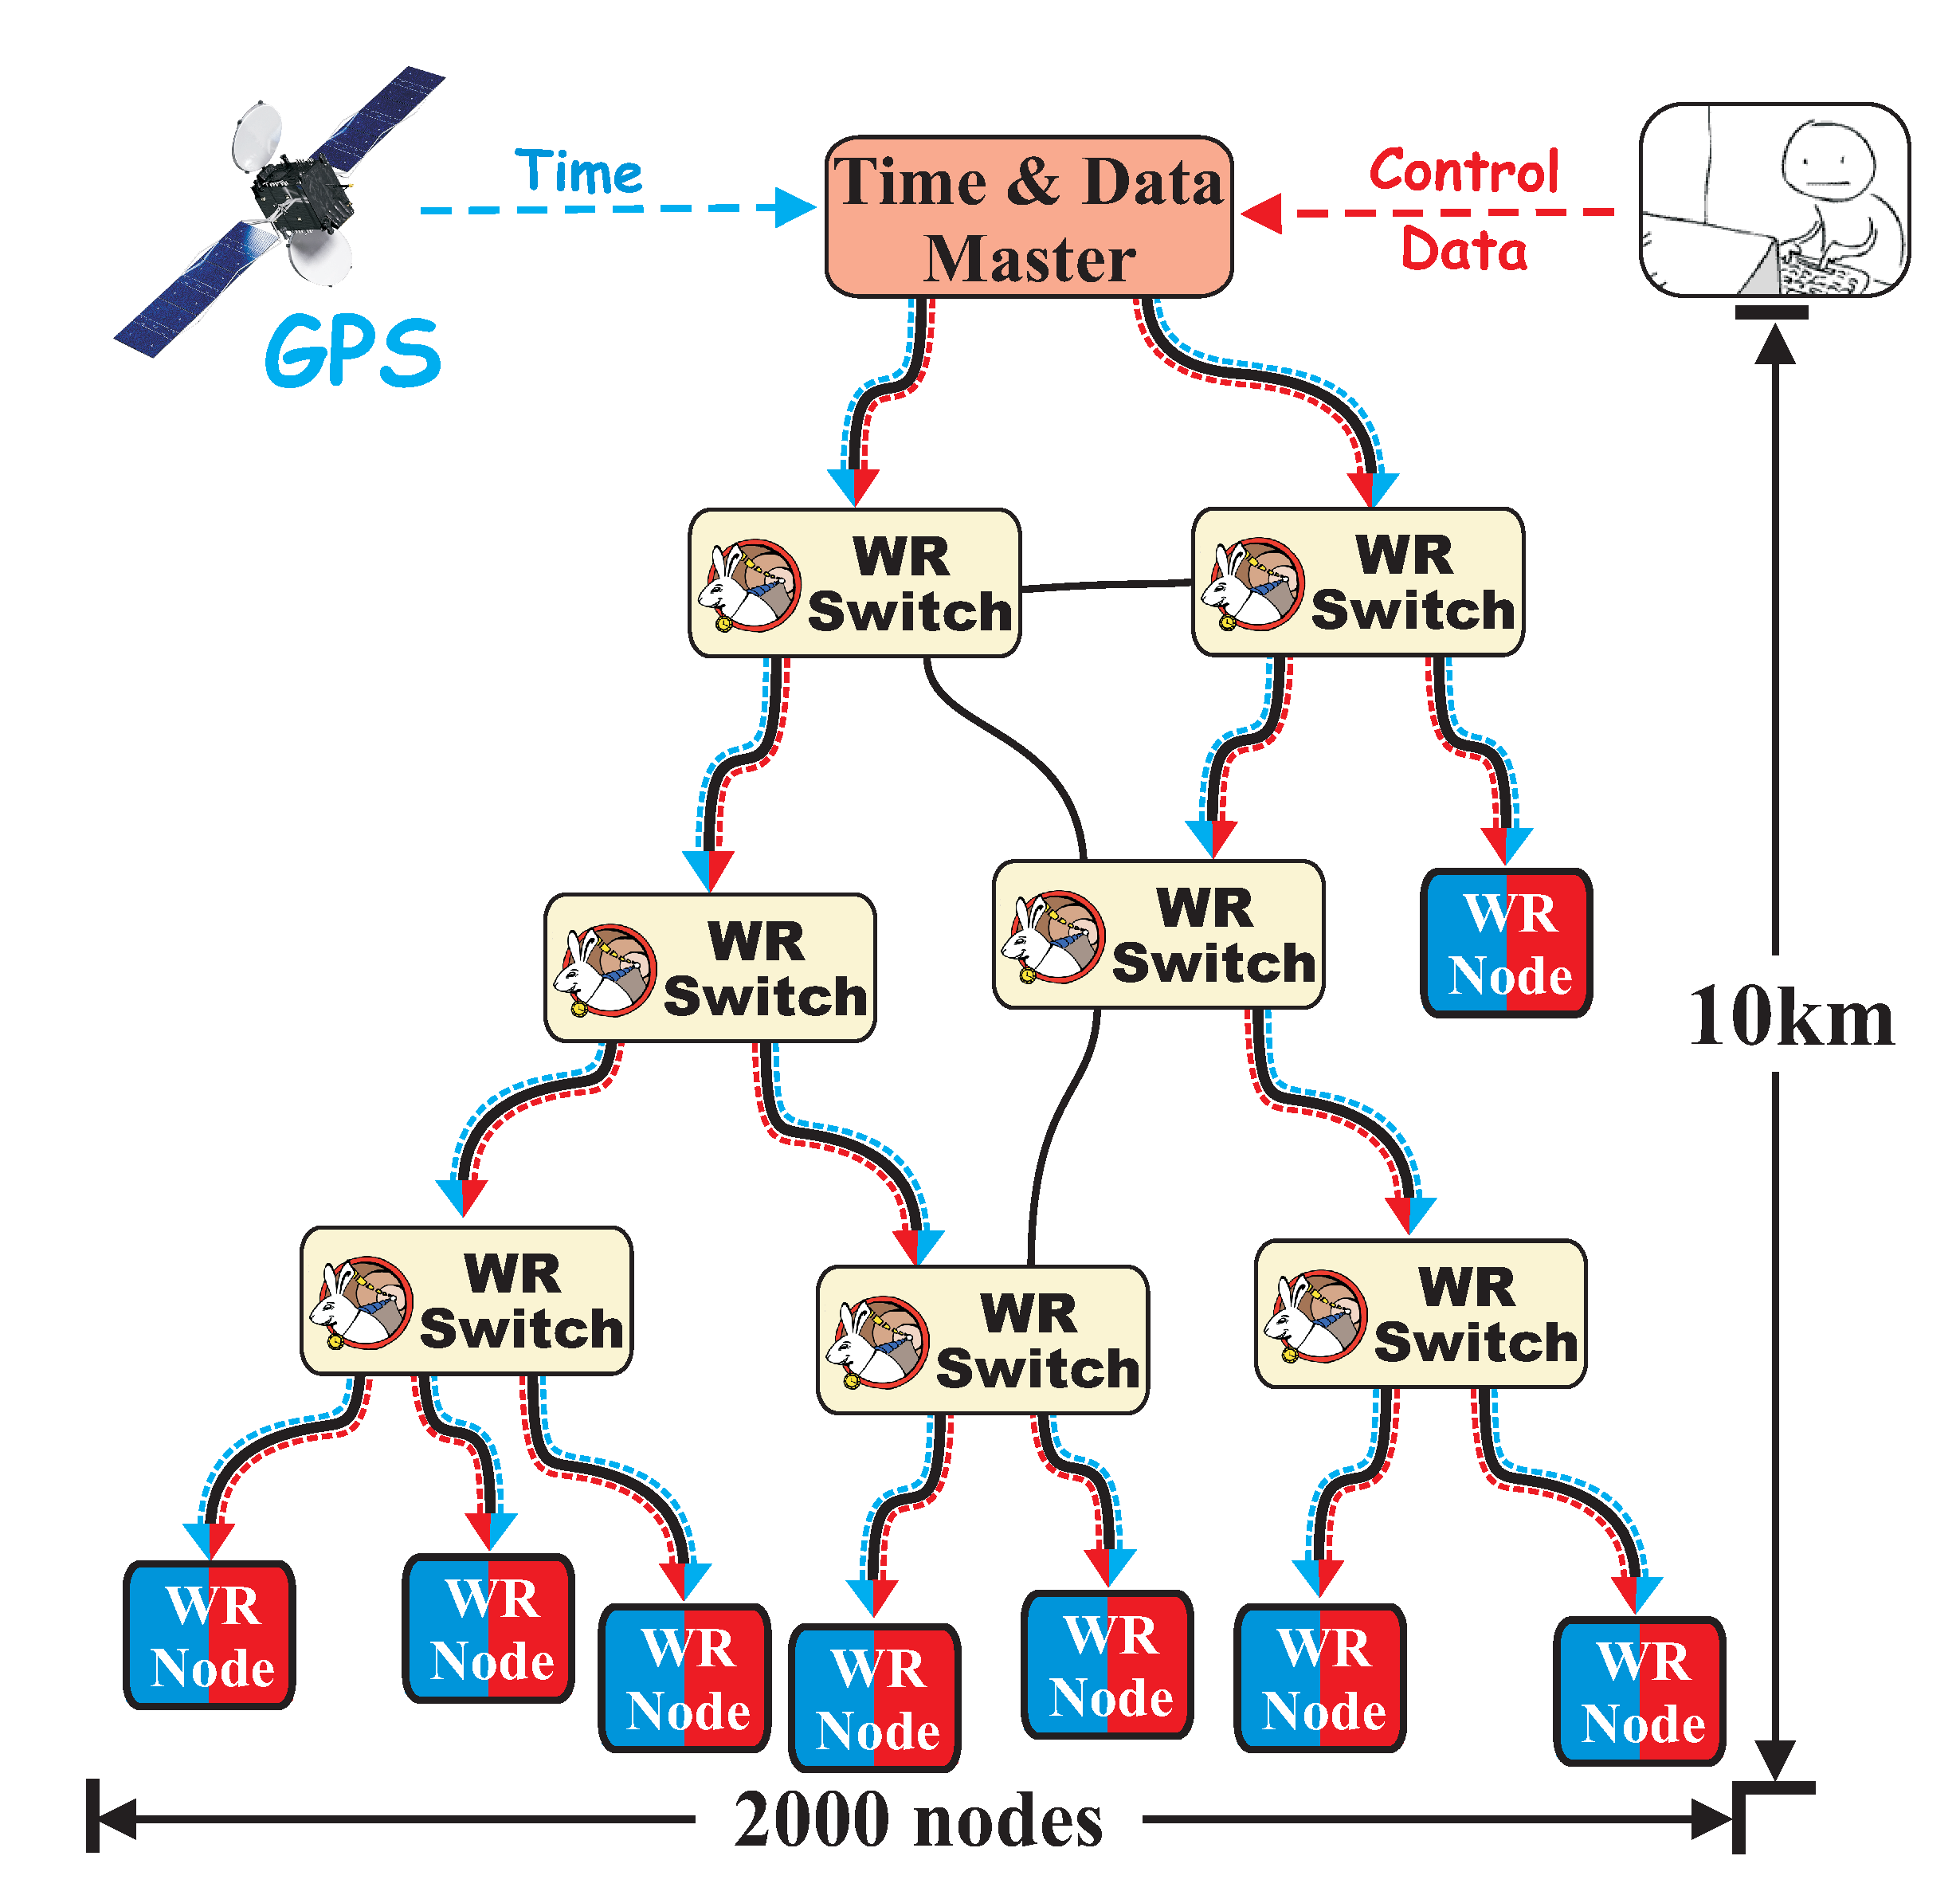
\includegraphics[height=1.0\textwidth]{../../figures/network/wr_network-new.ps}
    \end{center}
\end{columns}

\end{frame}
%%%%%%%%%%%%%%%%%%%%%%%%%%%%%%%%%%%%%%%%%%%%%%%%%%%%%%%%%%%%%%%%%%%%%%%%%%%%%%%%%%%%%%%%%%%%%%%%%%%%
%\section{Status}
%\subsection{}
%%%%%%%%%%%%%%%%%%%%%%%%%%%%%%%%%%%%%%%%%%%%%%%%%%%%%%%%%%%%%%%%%%%%%%%%%%%%%%%%%%%%%%%%%%%%%%%%%%%%
\begin{frame}{Data Distribution in WR Control System}

    \begin{center}
%     \includegraphics<1>[width=1.1\textwidth]{../../figures/applications/CERN/WRControlNetwork.ps} \pause
    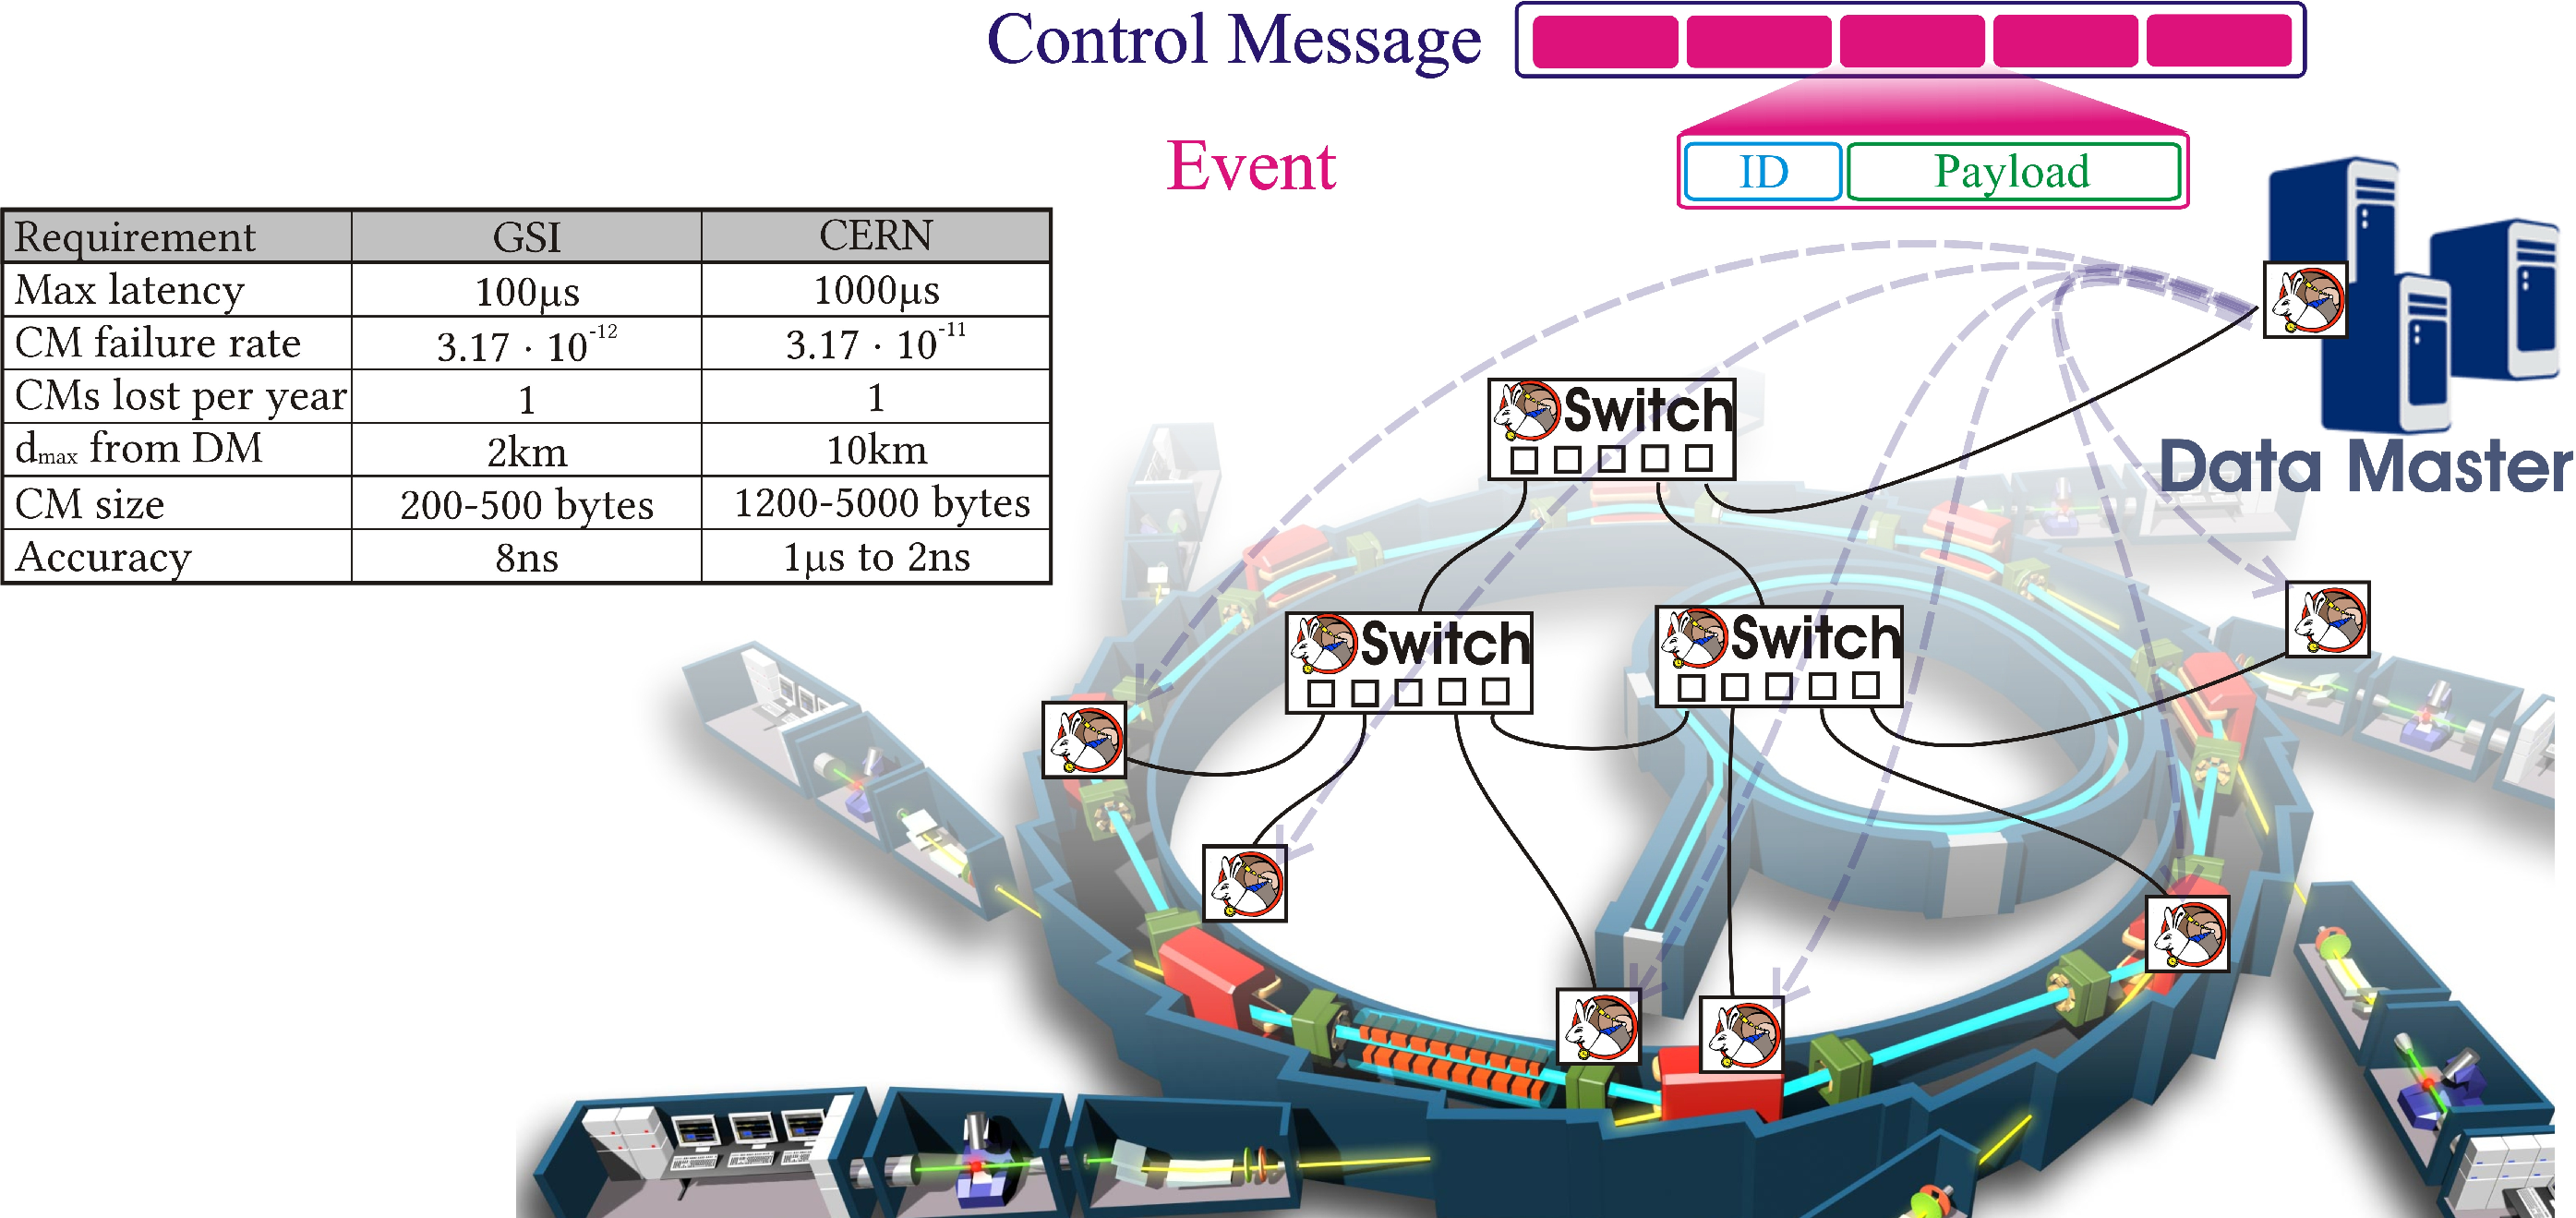
\includegraphics[width=1.1\textwidth]{../../figures/applications/CERN/WRControlNetwork2.ps}
    \end{center}


\end{frame}
%%%%%%%%%%%%%%%%%%%%%%%%%%%%%%%%%%%%%%%%%%%%%%%%%%%%%%%%%%%%%%%%%%%%%%%%%%%%%%%%%%%%%%%%%%%%%%%%%%%%
%\section{Status}
%\subsection{}
%%%%%%%%%%%%%%%%%%%%%%%%%%%%%%%%%%%%%%%%%%%%%%%%%%%%%%%%%%%%%%%%%%%%%%%%%%%%%%%%%%%%%%%%%%%%%%%%%%%%
\begin{frame}{Control Data}

\begin{columns}[c]
  \column{.62\textwidth}
    \begin{itemize}
      \item Two types of data:
	  \begin{itemize}
	    \item \textcolor{red}{\bf Control Data} (High Priority, HP)
	    \item Standard Data (Best Effort)
	  \end{itemize}
	  \item Characteristics of \textcolor{red}{\bf Control Data}
	  \begin{itemize}
	    \item Sent in Control Messages
	    \item Sent by Data Master(s)
	    \item Broadcast/Multicast (one-to-alot)
	    \item Deterministic and low latency
	    \item Reliable delivery
	  \end{itemize}
    \end{itemize}
  \column{.6\textwidth}
   % \vspace{-1cm}
   % \hspace{-6cm}
    \begin{center}
    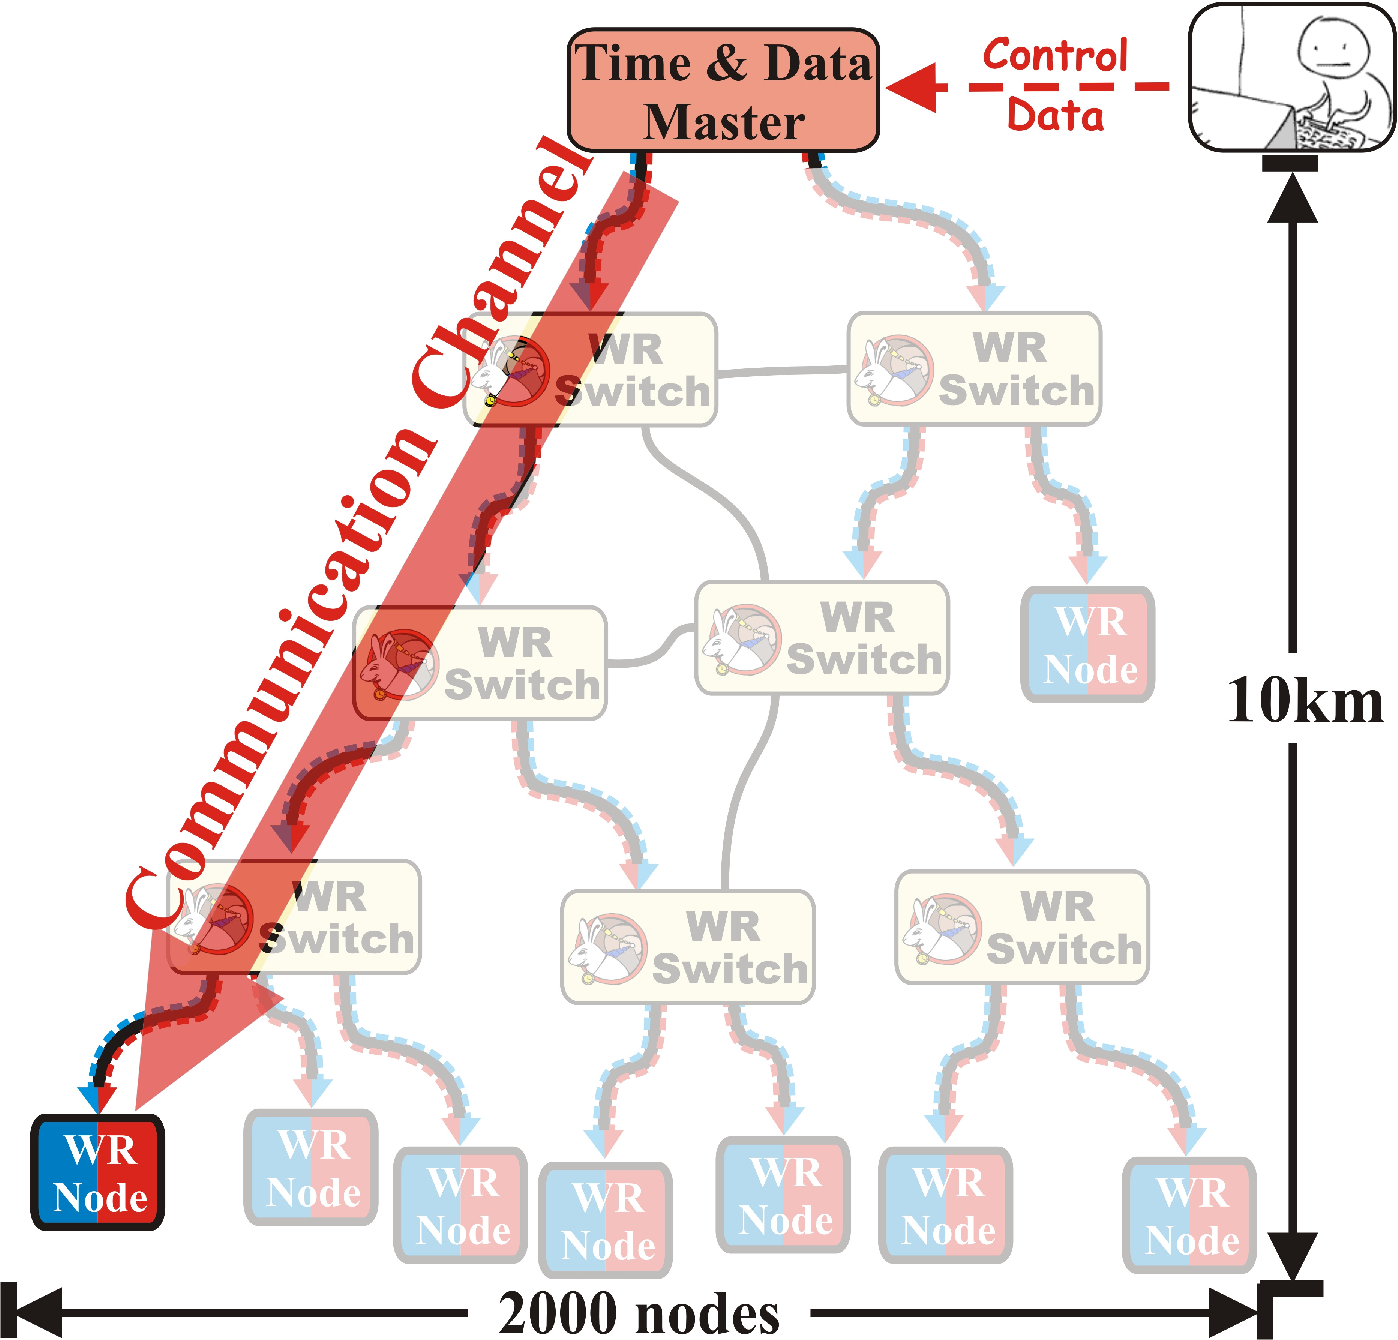
\includegraphics[height=0.6\textheight]{../../figures/robustness/CommunicationChannel.ps}
    \end{center}

\end{columns}

\end{frame}
%%%%%%%%%%%%%%%%%%%%%%%%%%%%%%%%%%%%%%%%%%%%%%%%%%%%%%%%%%%%%%%%%%%%%%%%%%%%%%%%%%%%%%%%%%%%%%%%%%%%
%\section{}
%\subsection{Data Redundancy}
%%%%%%%%%%%%%%%%%%%%%%%%%%%%%%%%%%%%%%%%%%%%%%%%%%%%%%%%%%%%%%%%%%%%%%%%%%%%%%%%%%%%%%%%%%%%%%%%%%%%
\begin{frame}{Data Redundancy}

  \begin{itemize}
    \item Re-transmission of Control Data not possible
	\item {\bf Forward Error Correction}  -- additional transparent layer:
	\begin{itemize}
		\item One Control Message encoded into N Ethernet frames,
		\item Recovery of Control Message from any M (M$<$N) frames
	\end{itemize}
	\item FEC can prevent data loss due to:
	\begin{itemize}	
		\item {\bf bit error} 
		\item {\bf network reconfiguration}
	\end{itemize}	
  \end{itemize}
  
  	\begin{center}
      
\includegraphics[width=.7\textwidth]{../../figures/robustness/FEC.eps}
    \end{center}
  
\end{frame}
%%%%%%%%%%%%%%%%%%%%%%%%%%%%%%%%%%%%%%%%%%%%%%%%%%%%%%%%%%%%%%%%%%%%%%%%%%%%%%%%%%%%%%%%%%%%%%%%%%%%
%\section{}
%\subsection{Topology Redundancy}
%%%%%%%%%%%%%%%%%%%%%%%%%%%%%%%%%%%%%%%%%%%%%%%%%%%%%%%%%%%%%%%%%%%%%%%%%%%%%%%%%%%%%%%%%%%%%%%%%%%%
\begin{frame}{Topology Redundancy}

\begin{columns}[c]
  \column{0.65\textwidth}

      \begin{itemize}
	    \item Standard Ethernet solution: Rapid/Multi Spanning Tree Protocol
	    \item Reconfiguration time: \textbf{$\approx$ 1s} \\ (best: milliseconds)
	    \item \textbf{1s = $\approx$ 82 000} Ethernet Frames lost
	    \item Solution:
	    \begin{itemize}
		  \item take advantage of FEC
		  \item speed up (R/M)STP$->$\textbf{eRSTP} or
		  \item use multiple paths$->$\textbf{eLACP}
	    \end{itemize}

      \end{itemize}
% 
  \column{0.6\textwidth}
    \begin{center}
    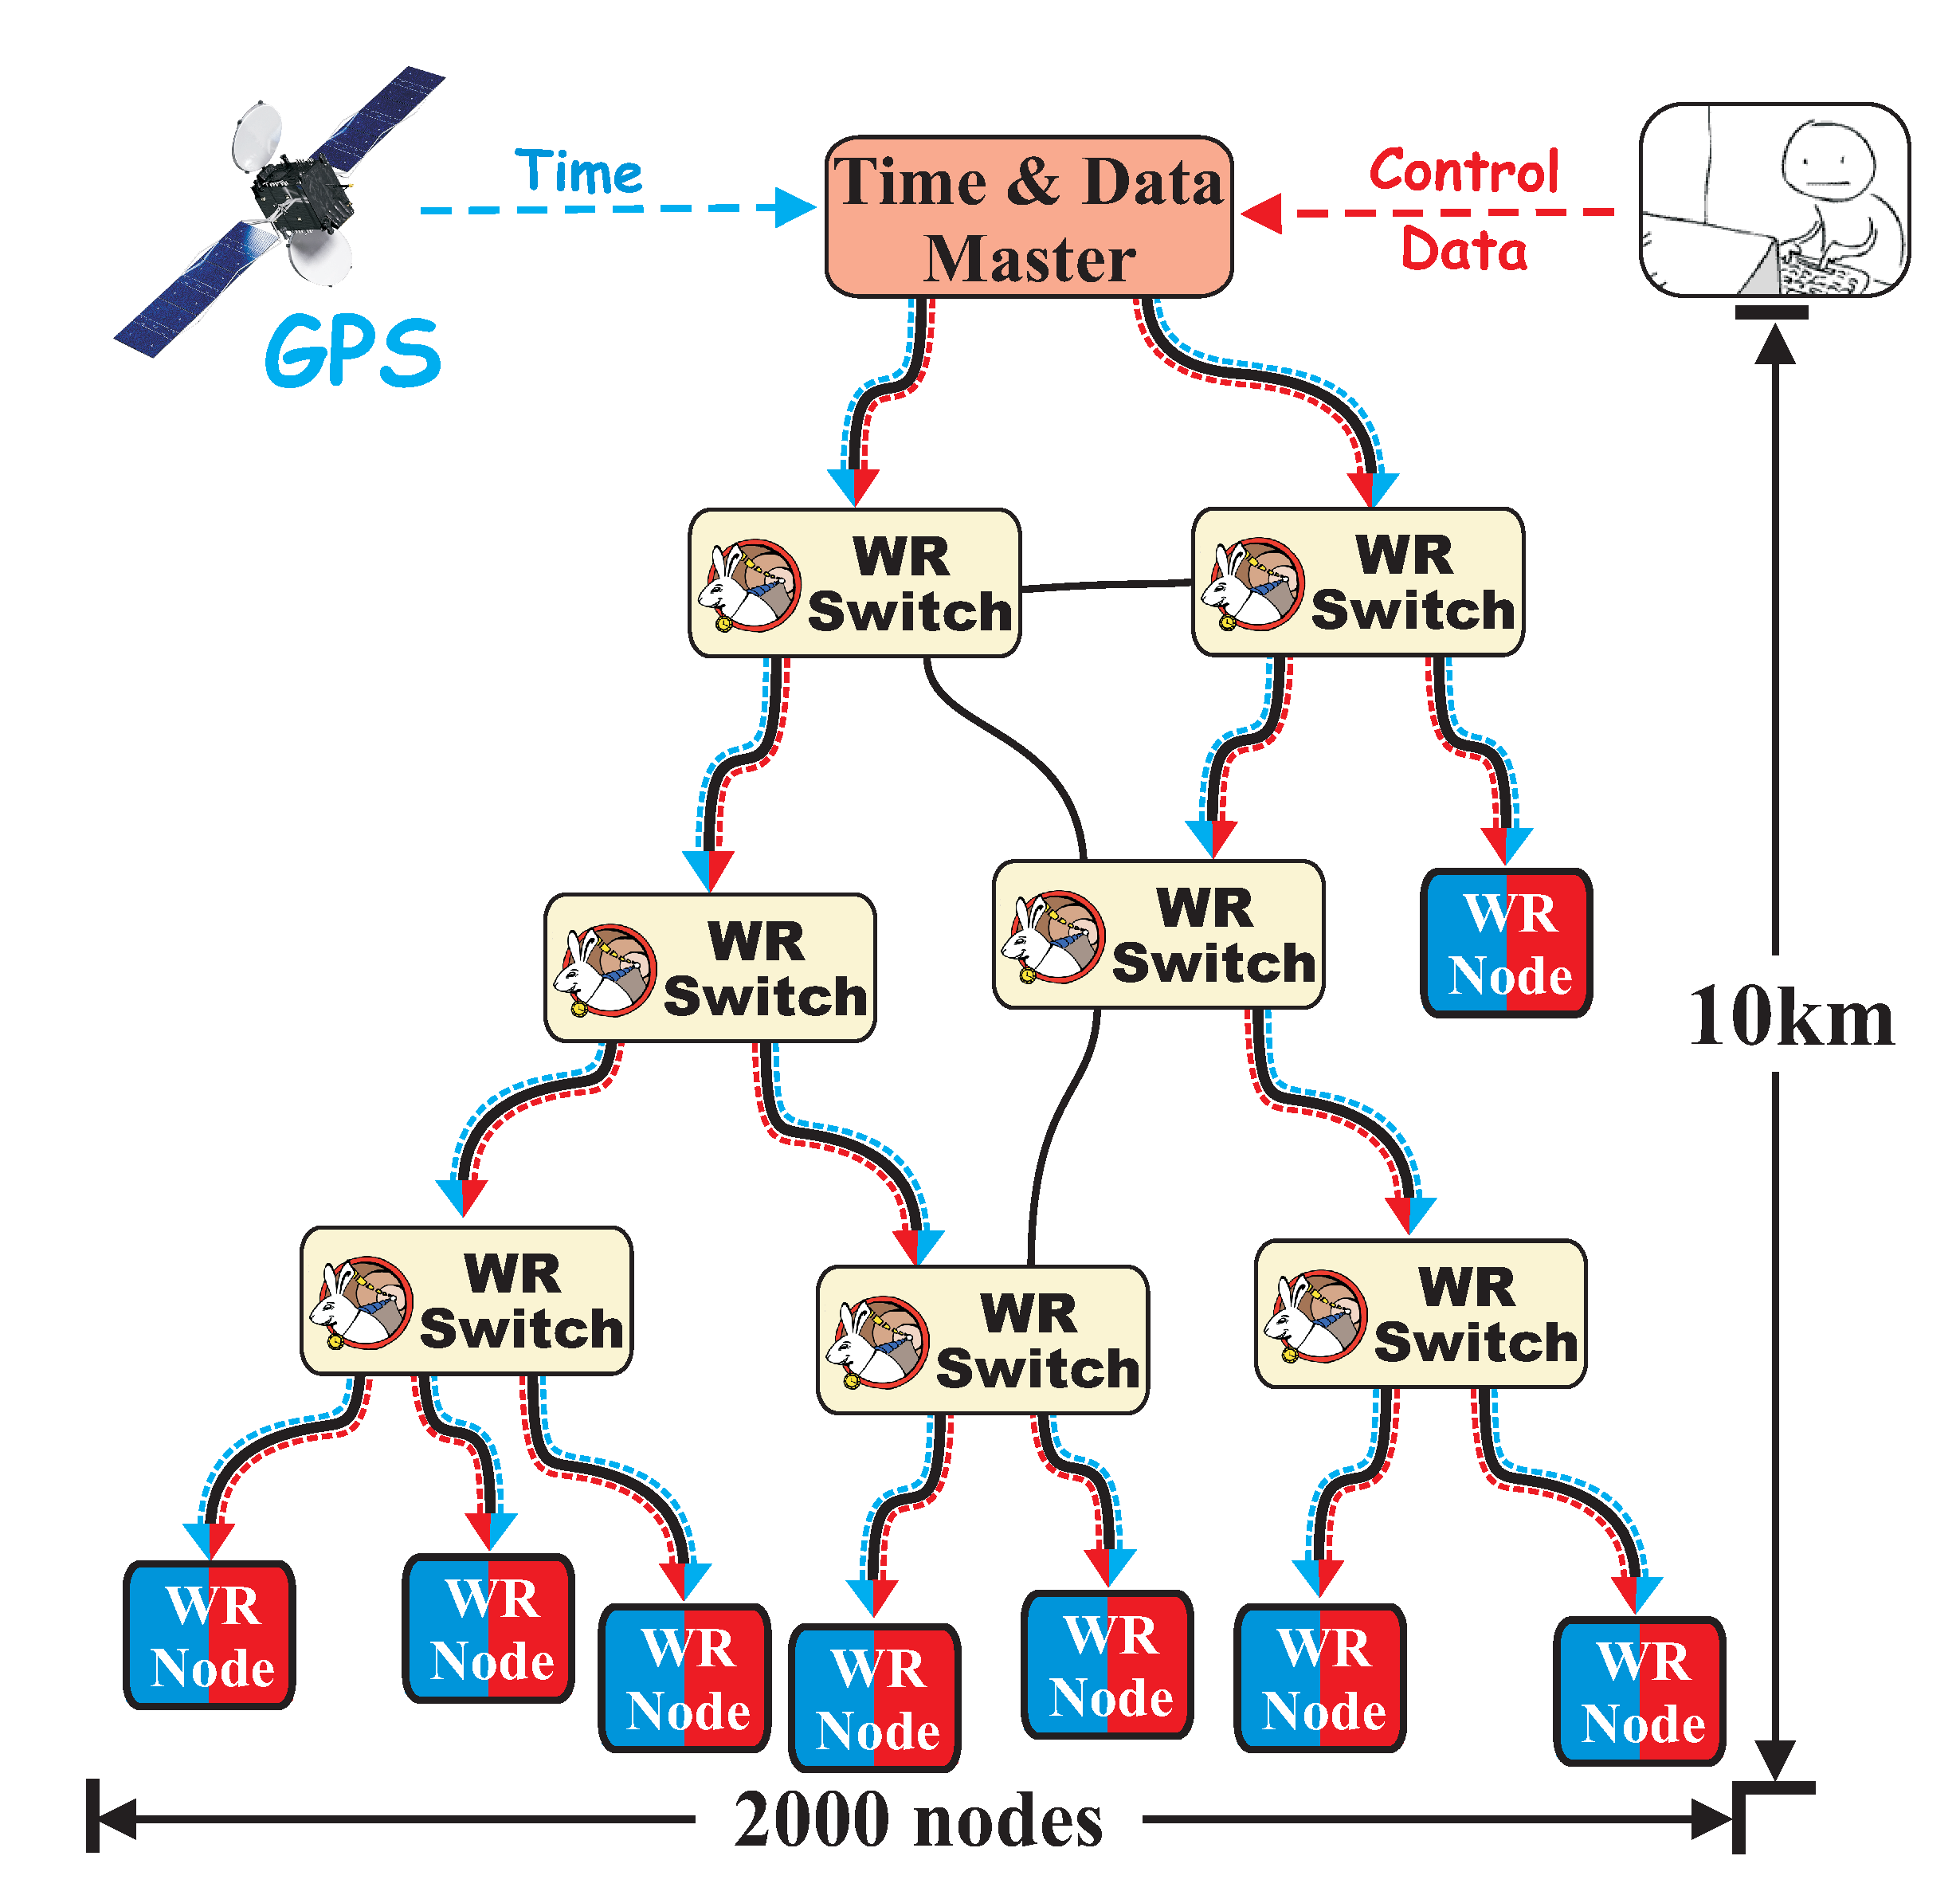
\includegraphics[width=0.65\textwidth]{../../figures/network/wr_network-new.ps}
    \end{center}
\end{columns}

\end{frame}
%%%%%%%%%%%%%%%%%%%%%%%%%%%%%%%%%%%%%%%%%%%%%%%%%%%%%%%%%%%%%%%%%%%%%%%%%%%%%%%%%%%%%%%%%%%%%%%%%%%%
%\section{}
%\subsection{Topology Redundancy}
%%%%%%%%%%%%%%%%%%%%%%%%%%%%%%%%%%%%%%%%%%%%%%%%%%%%%%%%%%%%%%%%%%%%%%%%%%%%%%%%%%%%%%%%%%%%%%%%%%%%
\begin{frame}{Determinism and Low Latency}

\begin{columns}[c]
  \column{0.6\textwidth}

      \begin{itemize}
	    \item \textcolor{red}{Control Data}: \\$7^{th}$ Class of Service (priority)
	    \item WR Switch:
	    \begin{itemize}
	      \item Quality of Service: resource reservation
	      \item Upper bound latency \\ by design: $<10us$
	      \item Cut-through
	    \end{itemize}
	    \item Careful diagnostics
      \end{itemize}
% 
  \column{0.6\textwidth}
    \begin{center}
%     \includegraphics<1>[width=0.65\textwidth]{../../figures/network/wr_network-new.ps} \pause
    \includegraphics[width=0.9\textwidth]{../../figures/robustness/event3.eps} 
    \end{center}

\end{columns}

\end{frame}
%%%%%%%%%%%%%%%%%%%%%%%%%%%%%%%%%%%%%%%%%%%%%%%%%%%%%%%%%%%%%%%%%%%%%%%%%%%%%%%%%%%%%%%%%%%%%%%%%%%%
%\section{}
%\subsection{Topology Redundancy}
% %%%%%%%%%%%%%%%%%%%%%%%%%%%%%%%%%%%%%%%%%%%%%%%%%%%%%%%%%%%%%%%%%%%%%%%%%%%%%%%%%%%%%%%%%%%%%%%%%%%%
% \begin{frame}{Data Distribution summary}
% 
% \small
%   \begin{itemize}
%     \item Optional feature
%     \item Openness enables everyone to verify the parameters
%     \item Ongoing efforts (2012/2013)
%     \item Commonalities with IEEE effort for $2^{nd}$ gen Audio~Video~Bridging 
%   \end{itemize}
% 
% \end{frame}
%%%%%%%%%%%%%%%%%%%%%%%%%%%%%%%%%%%%%%%%%%%%%%%%%%%%%%%%%%%%%%%%%%%%%%%%%%%%%%%%%%%%%%%%%%%%%%%%%%%%
\section{Components}
\subsection{}
%%%%%%%%%%%%%%%%%%%%%%%%%%%%%%%%%%%%%%%%%%%%%%%%%%%%%%%%%%%%%%%%%%%%%%%%%%%%%%%%%%%%%%%%%%%%%%%%%%%%
\begin{frame}{White Rabbit Network Components}


    \begin{center}
    %\includegraphics<1>[width=1.0\textwidth]{fig/WRNcomponents.eps}  \pause
    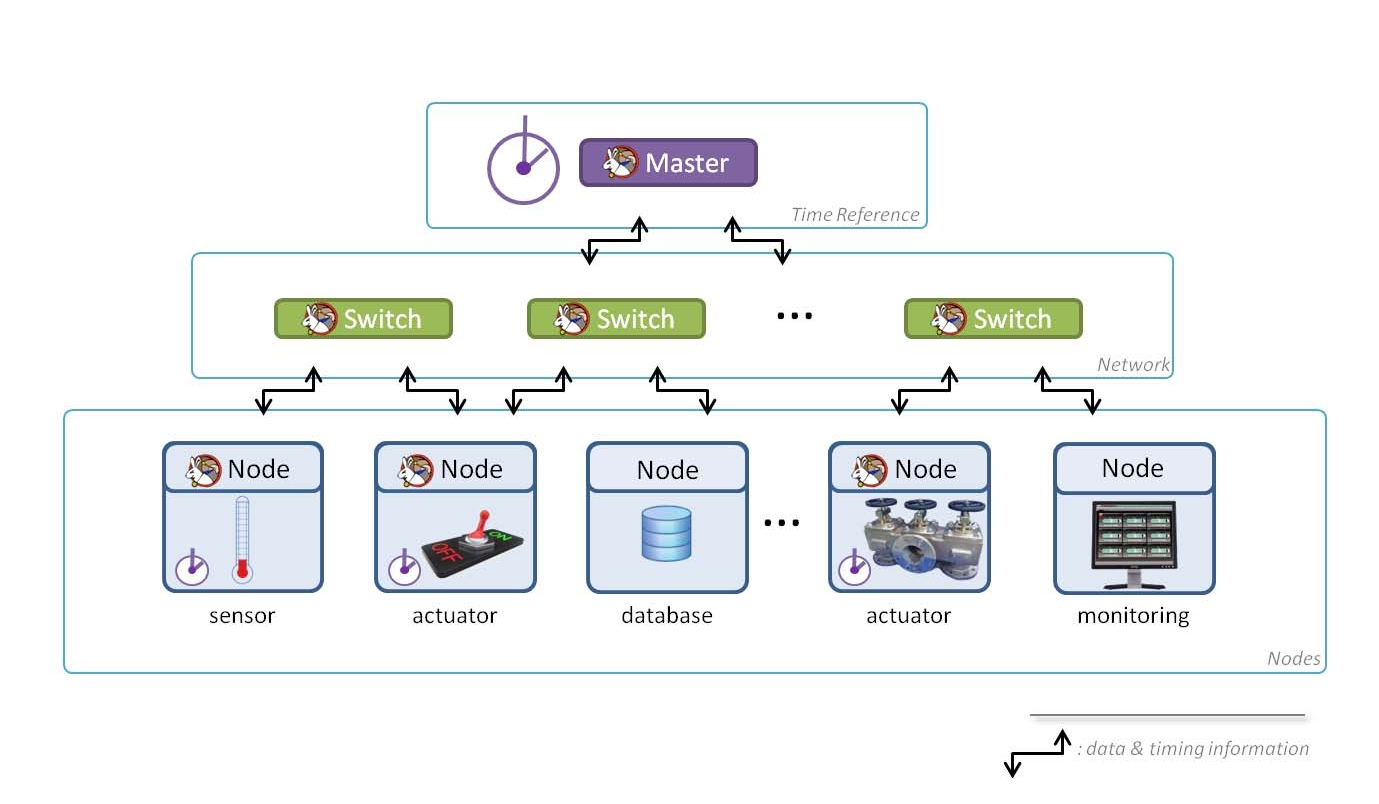
\includegraphics[width=1.0\textwidth]{../../figures/network/WRnetwork-eva.eps}  
%     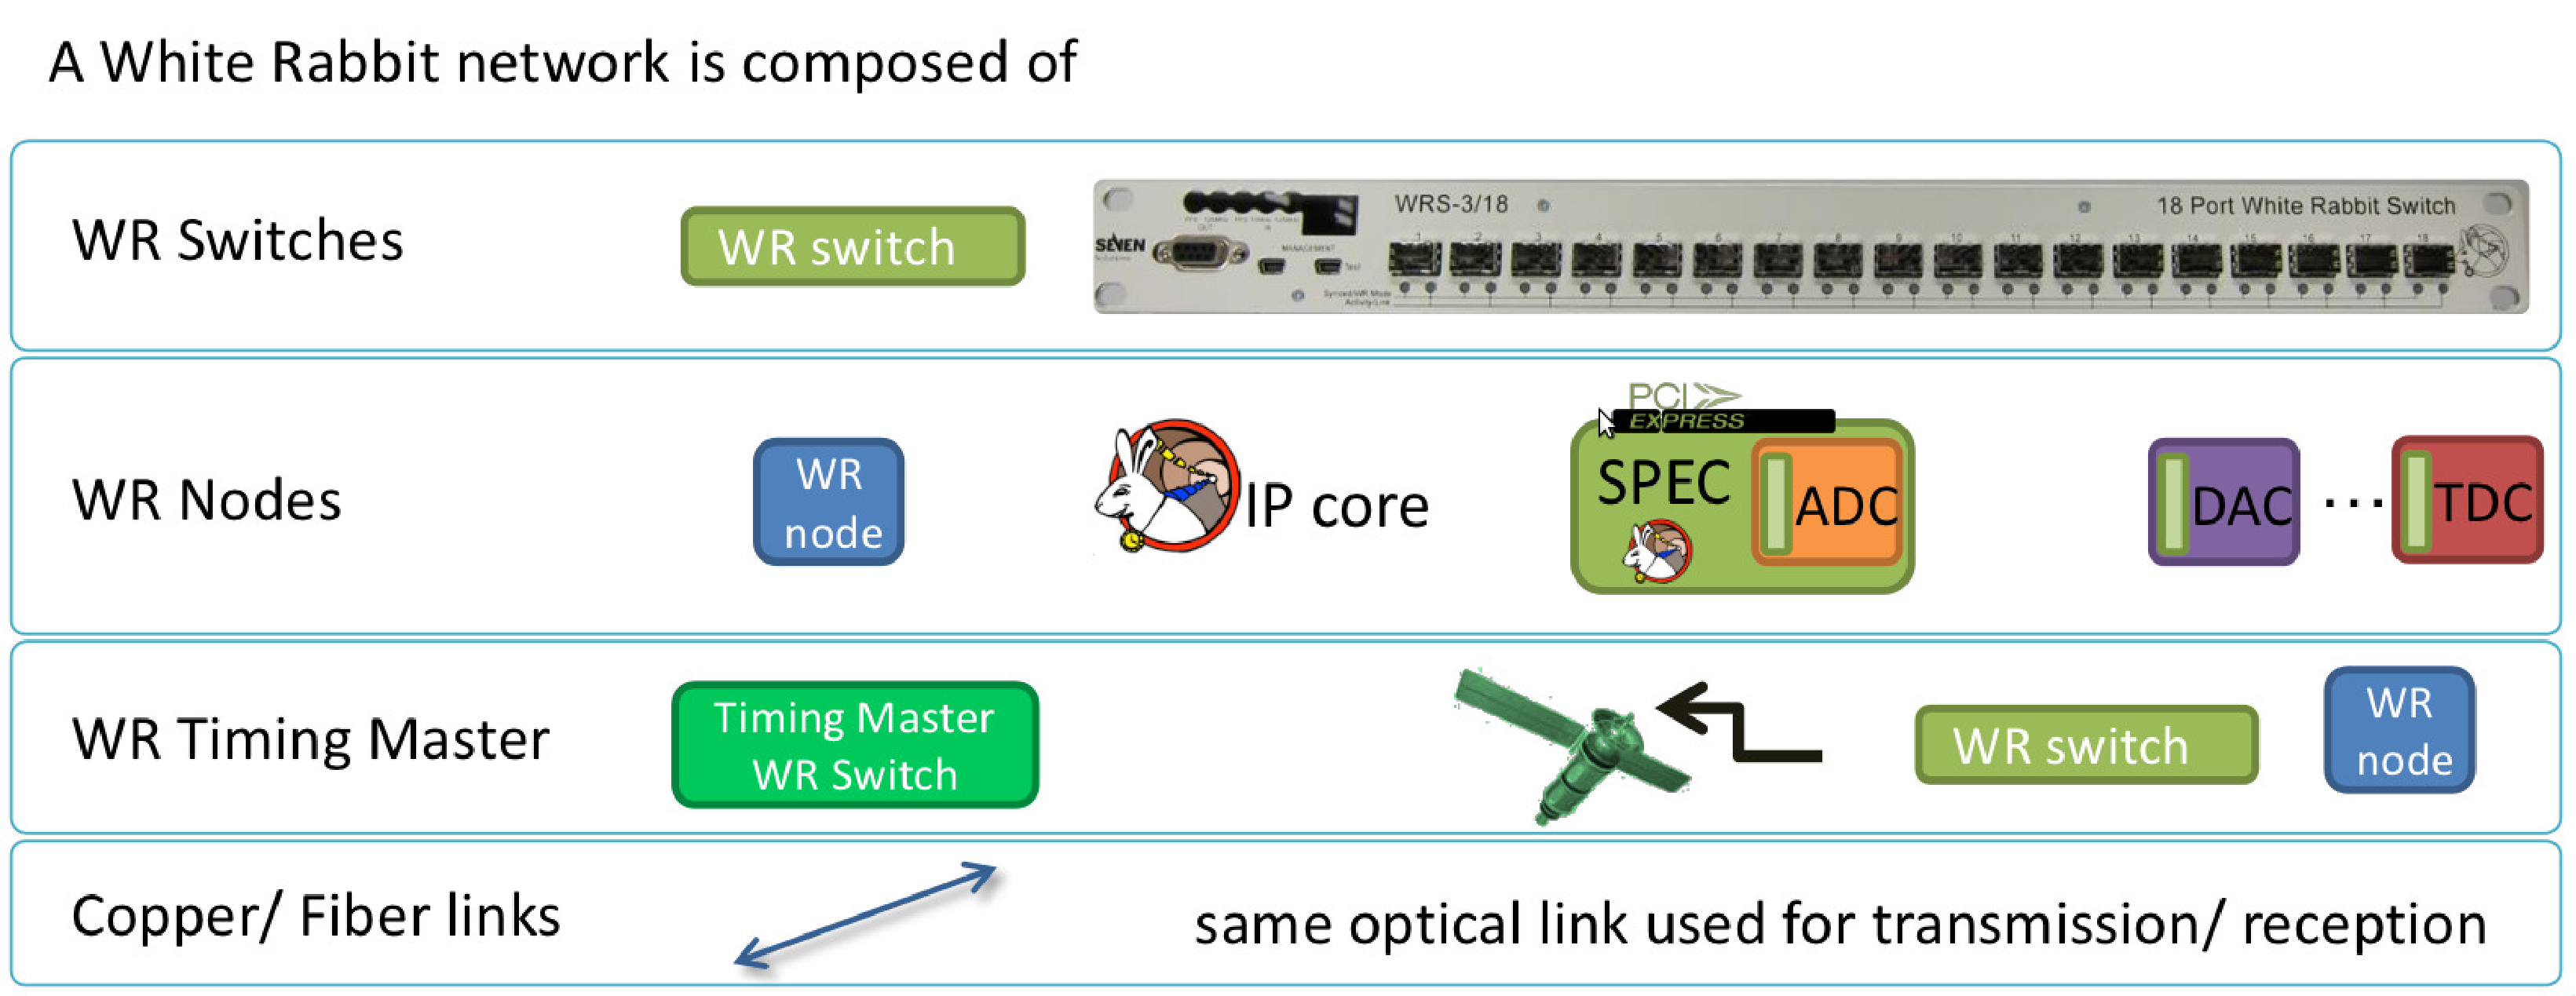
\includegraphics[width=1.0\textwidth]{figs/WRNcomponents-2.eps}
    \end{center}

\end{frame}
%%%%%%%%%%%%%%%%%%%%%%%%%%%%%%%%%%%%%%%%%%%%%%%%%%%%%%%%%%%%%%%%%%%%%%%%%%%%%%%%%%%%%%%%%%%%%%%%%%%%
%\section{}
%\subsection{Topology Redundancy}
%%%%%%%%%%%%%%%%%%%%%%%%%%%%%%%%%%%%%%%%%%%%%%%%%%%%%%%%%%%%%%%%%%%%%%%%%%%%%%%%%%%%%%%%%%%%%%%%%%%%
\begin{frame}{White Rabbit Switch (V3)}

    \begin{center}
    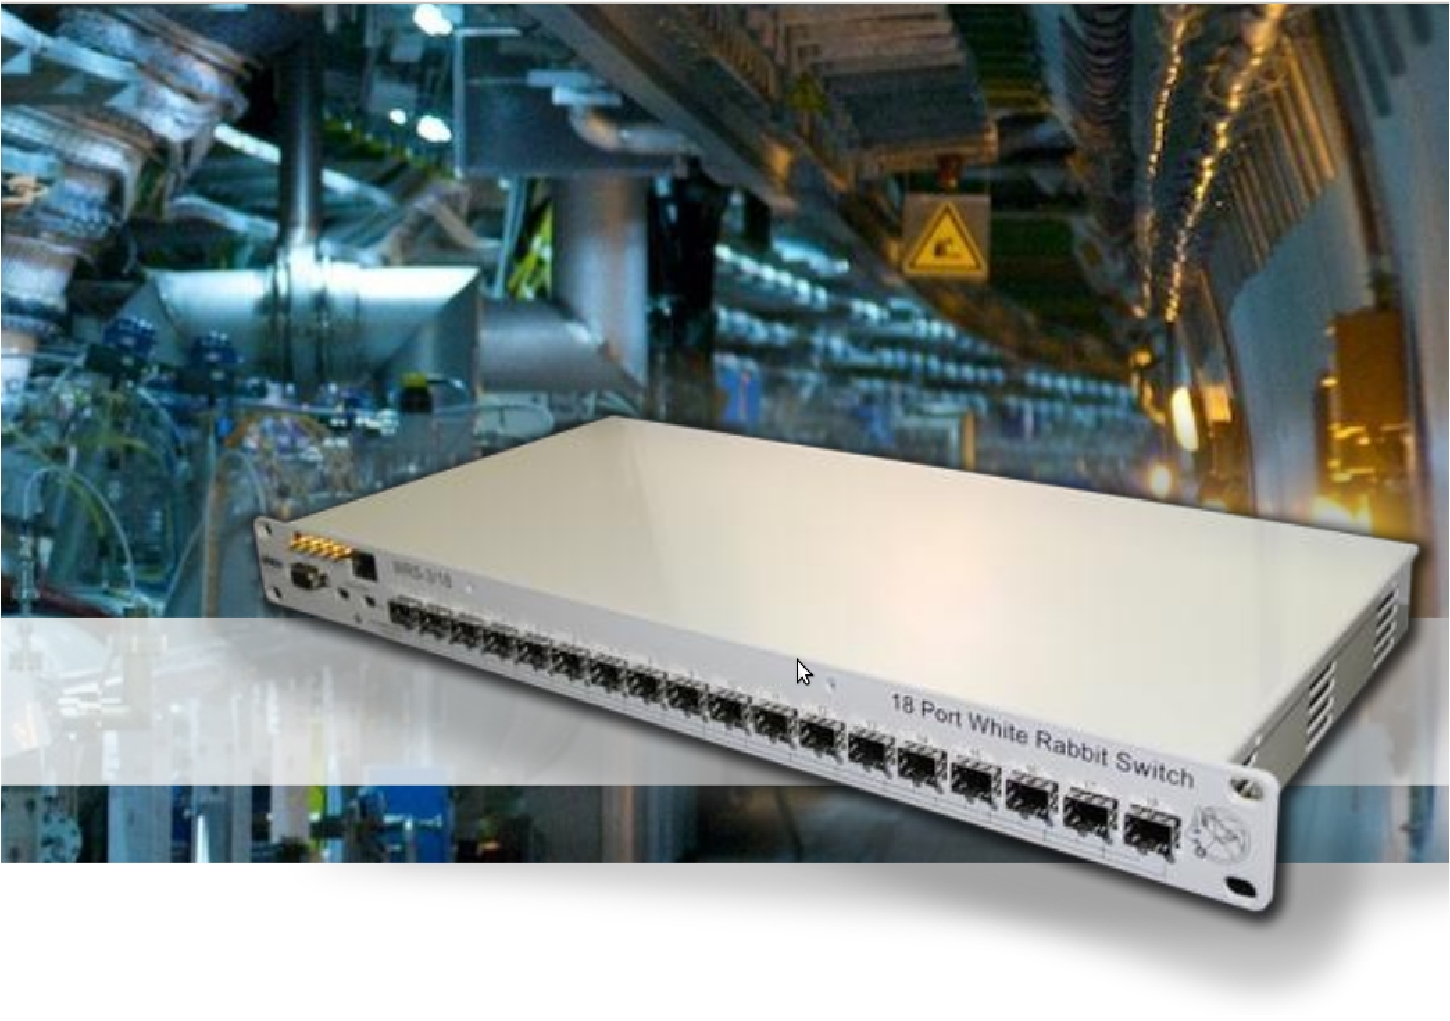
\includegraphics[width=6.0cm]{../../figures/switch/wrSwitchV3.ps}
    \end{center}

	\begin{itemize}
	\item Central element of WR network
	\item Original design optimized for timing, designed from scratch
	\item 18 1000BASE-BX10 ports
	\item Capable of driving 10 km of SM fiber
	\item Open design (H/W and S/W)
%	\item 200 ps synchronization accuracy
	\end{itemize}

\end{frame}
%%%%%%%%%%%%%%%%%%%%%%%%%%%%%%%%%%%%%%%%%%%%%%%%%%%%%%%%%%%%%%%%%%%%%%%%%%%%%%%%%%%%%%%%%%%%%%%%%%%%
%\section{}
%\subsection{Topology Redundancy}
%%%%%%%%%%%%%%%%%%%%%%%%%%%%%%%%%%%%%%%%%%%%%%%%%%%%%%%%%%%%%%%%%%%%%%%%%%%%%%%%%%%%%%%%%%%%%%%%%%%%
\begin{frame}{WR Node: WR PTP Core}

    \begin{center}
    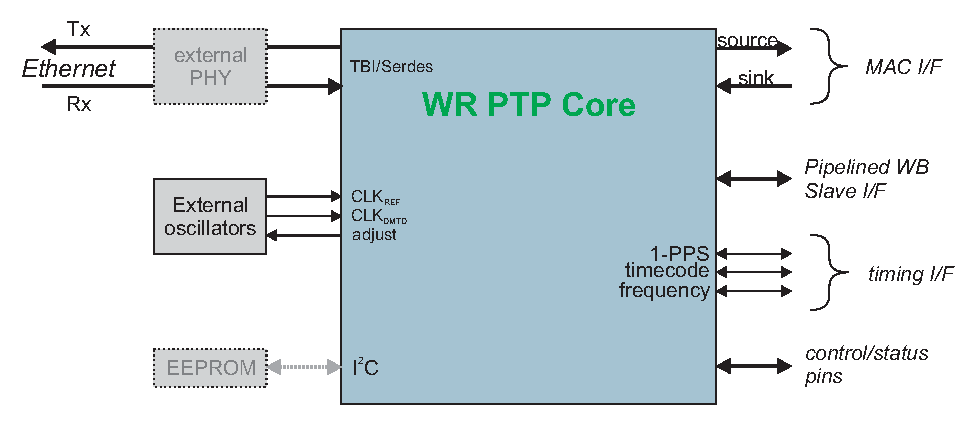
\includegraphics[width=1.0\textwidth]{../../figures/node/wrpc_box.eps}
    \end{center}

\end{frame}
%%%%%%%%%%%%%%%%%%%%%%%%%%%%%%%%%%%%%%%%%%%%%%%%%%%%%%%%%%%%%%%%%%%%%%%%%%%%%%%%%%%%%%%%%%%%%%%%%%%%
%\section{}
%\subsection{Topology Redundancy}
%%%%%%%%%%%%%%%%%%%%%%%%%%%%%%%%%%%%%%%%%%%%%%%%%%%%%%%%%%%%%%%%%%%%%%%%%%%%%%%%%%%%%%%%%%%%%%%%%%%%
\begin{frame}{WR Node: SPEC board}

    \begin{center}
    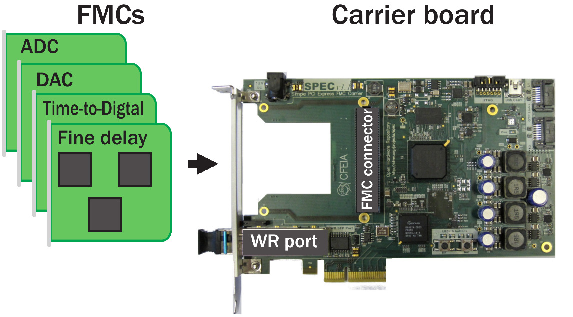
\includegraphics[width=7cm]{../../figures/node/shw_kit-1}
    \end{center}

  \begin{columns}[c]
    \column{.01\textwidth}
    \column{.98\textwidth}

	\begin{block}{Co-HT FMC-based Hardware Kit:}
%	\textbf{Co-HT FMC-based Hardware Kit:}
	  \begin{itemize}
	  \item FMCs (FPGA Mezzanine Cards) with ADCs, DACs, TDCs, fine delays, digital I/O
	  \item Carrier boards in PCI-Express, VME and uTCA formats
	  \item All carriers are equipped with a White Rabbit port
	  \end{itemize}
	\end{block}

    \column{.01\textwidth}
  \end{columns}


\end{frame}


%%%%%%%%%%%%%%%%%%%%%%%%%%%%%%%%%%%%%%%%%%%%%%%%%%%%%%%%%%%%%%%%%%%%%%%%%%%%%%%%%%%%%%%%%%%%%%%%%%%%
\section{Applications}
\subsection{}
%%%%%%%%%%%%%%%%%%%%%%%%%%%%%%%%%%%%%%%%%%%%%%%%%%%%%%%%%%%%%%%%%%%%%%%%%%%%%%%%%%%%%%%%%%%%%%%%%%%%
\begin{frame}{White Rabbit Applications}

    \begin{center}
      Much more than accelerator control and timing system ...
    \end{center}

%   \begin{itemize}
%     \item Control and timing system
%     \item Field bus recommended at CERN
%     \item Time Transfer
%     \item RF distribution
%     \item Distributed oscilloscope
%     \item ...
%   \end{itemize}

\end{frame}
%%%%%%%%%%%%%%%%%%%%%%%%%%%%%%%%%%%%%%%%%%%%%%%%%%%%%%%%%%%%%%%%%%%%%%%%%%%%%%%%%%%%%%%%%%%%%%%%%%%%
% \section{}
% \subsection{}
%%%%%%%%%%%%%%%%%%%%%%%%%%%%%%%%%%%%%%%%%%%%%%%%%%%%%%%%%%%%%%%%%%%%%%%%%%%%%%%%%%%%%%%%%%%%%%%%%%%%
\begin{frame}{WR at CERN}

      \begin{center}
      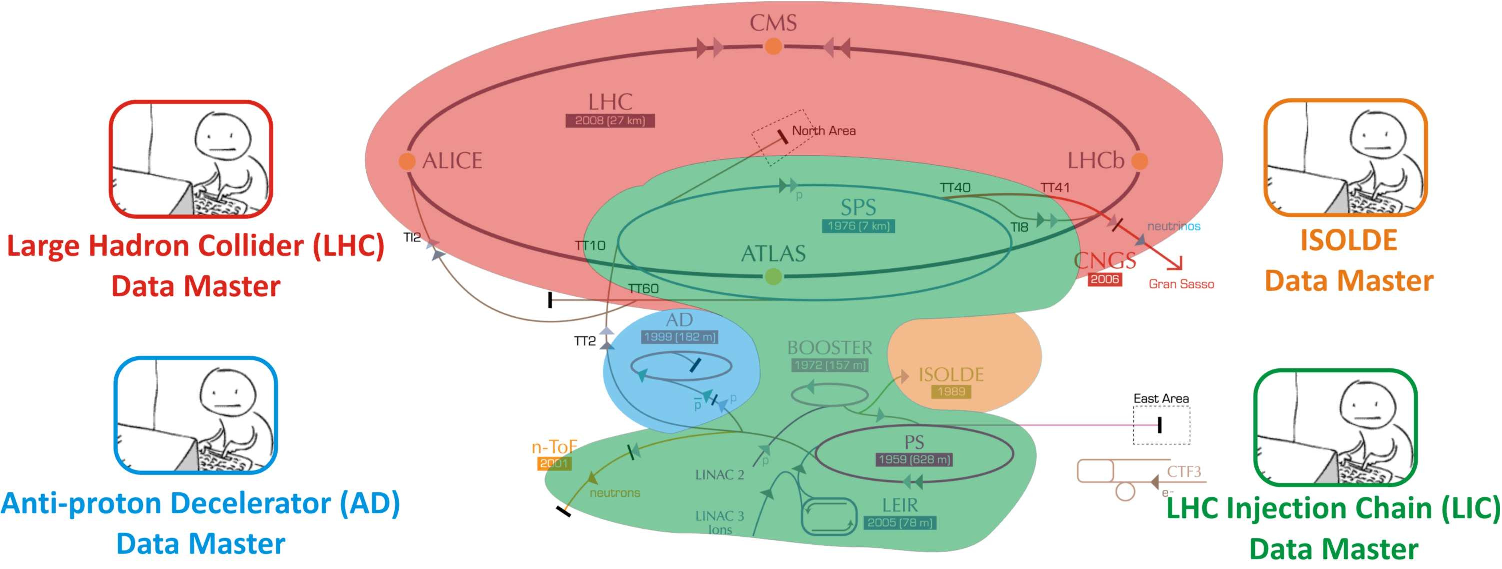
\includegraphics[width=.7\textwidth]{../../figures/applications/CERN/accNetworks.eps}
      \end{center}

  \begin{itemize}
    \item 4 accelerator networks
    \item Separate {\bf Data Master (DM)} for each network
    \item \textcolor{green!90}{LIC Data Master} communicates with other DMs and control devices in their networks
    \item Broadcast/Multicast of {\bf Control Messages} within network(s)
  \end{itemize}

\end{frame}
%%%%%%%%%%%%%%%%%%%%%%%%%%%%%%%%%%%%%%%%%%%%%%%%%%%%%%%%%%%%%%%%%%%%%%%%%%%%%%%%%%%%%%%%%%%%%%%%%%%%
%\section{WR-based Control System}
%\subsection{}
%%%%%%%%%%%%%%%%%%%%%%%%%%%%%%%%%%%%%%%%%%%%%%%%%%%%%%%%%%%%%%%%%%%%%%%%%%%%%%%%%%%%%%%%%%%%%%%%%%%%
\begin{frame}{WR at CERN}

    \begin{center}
      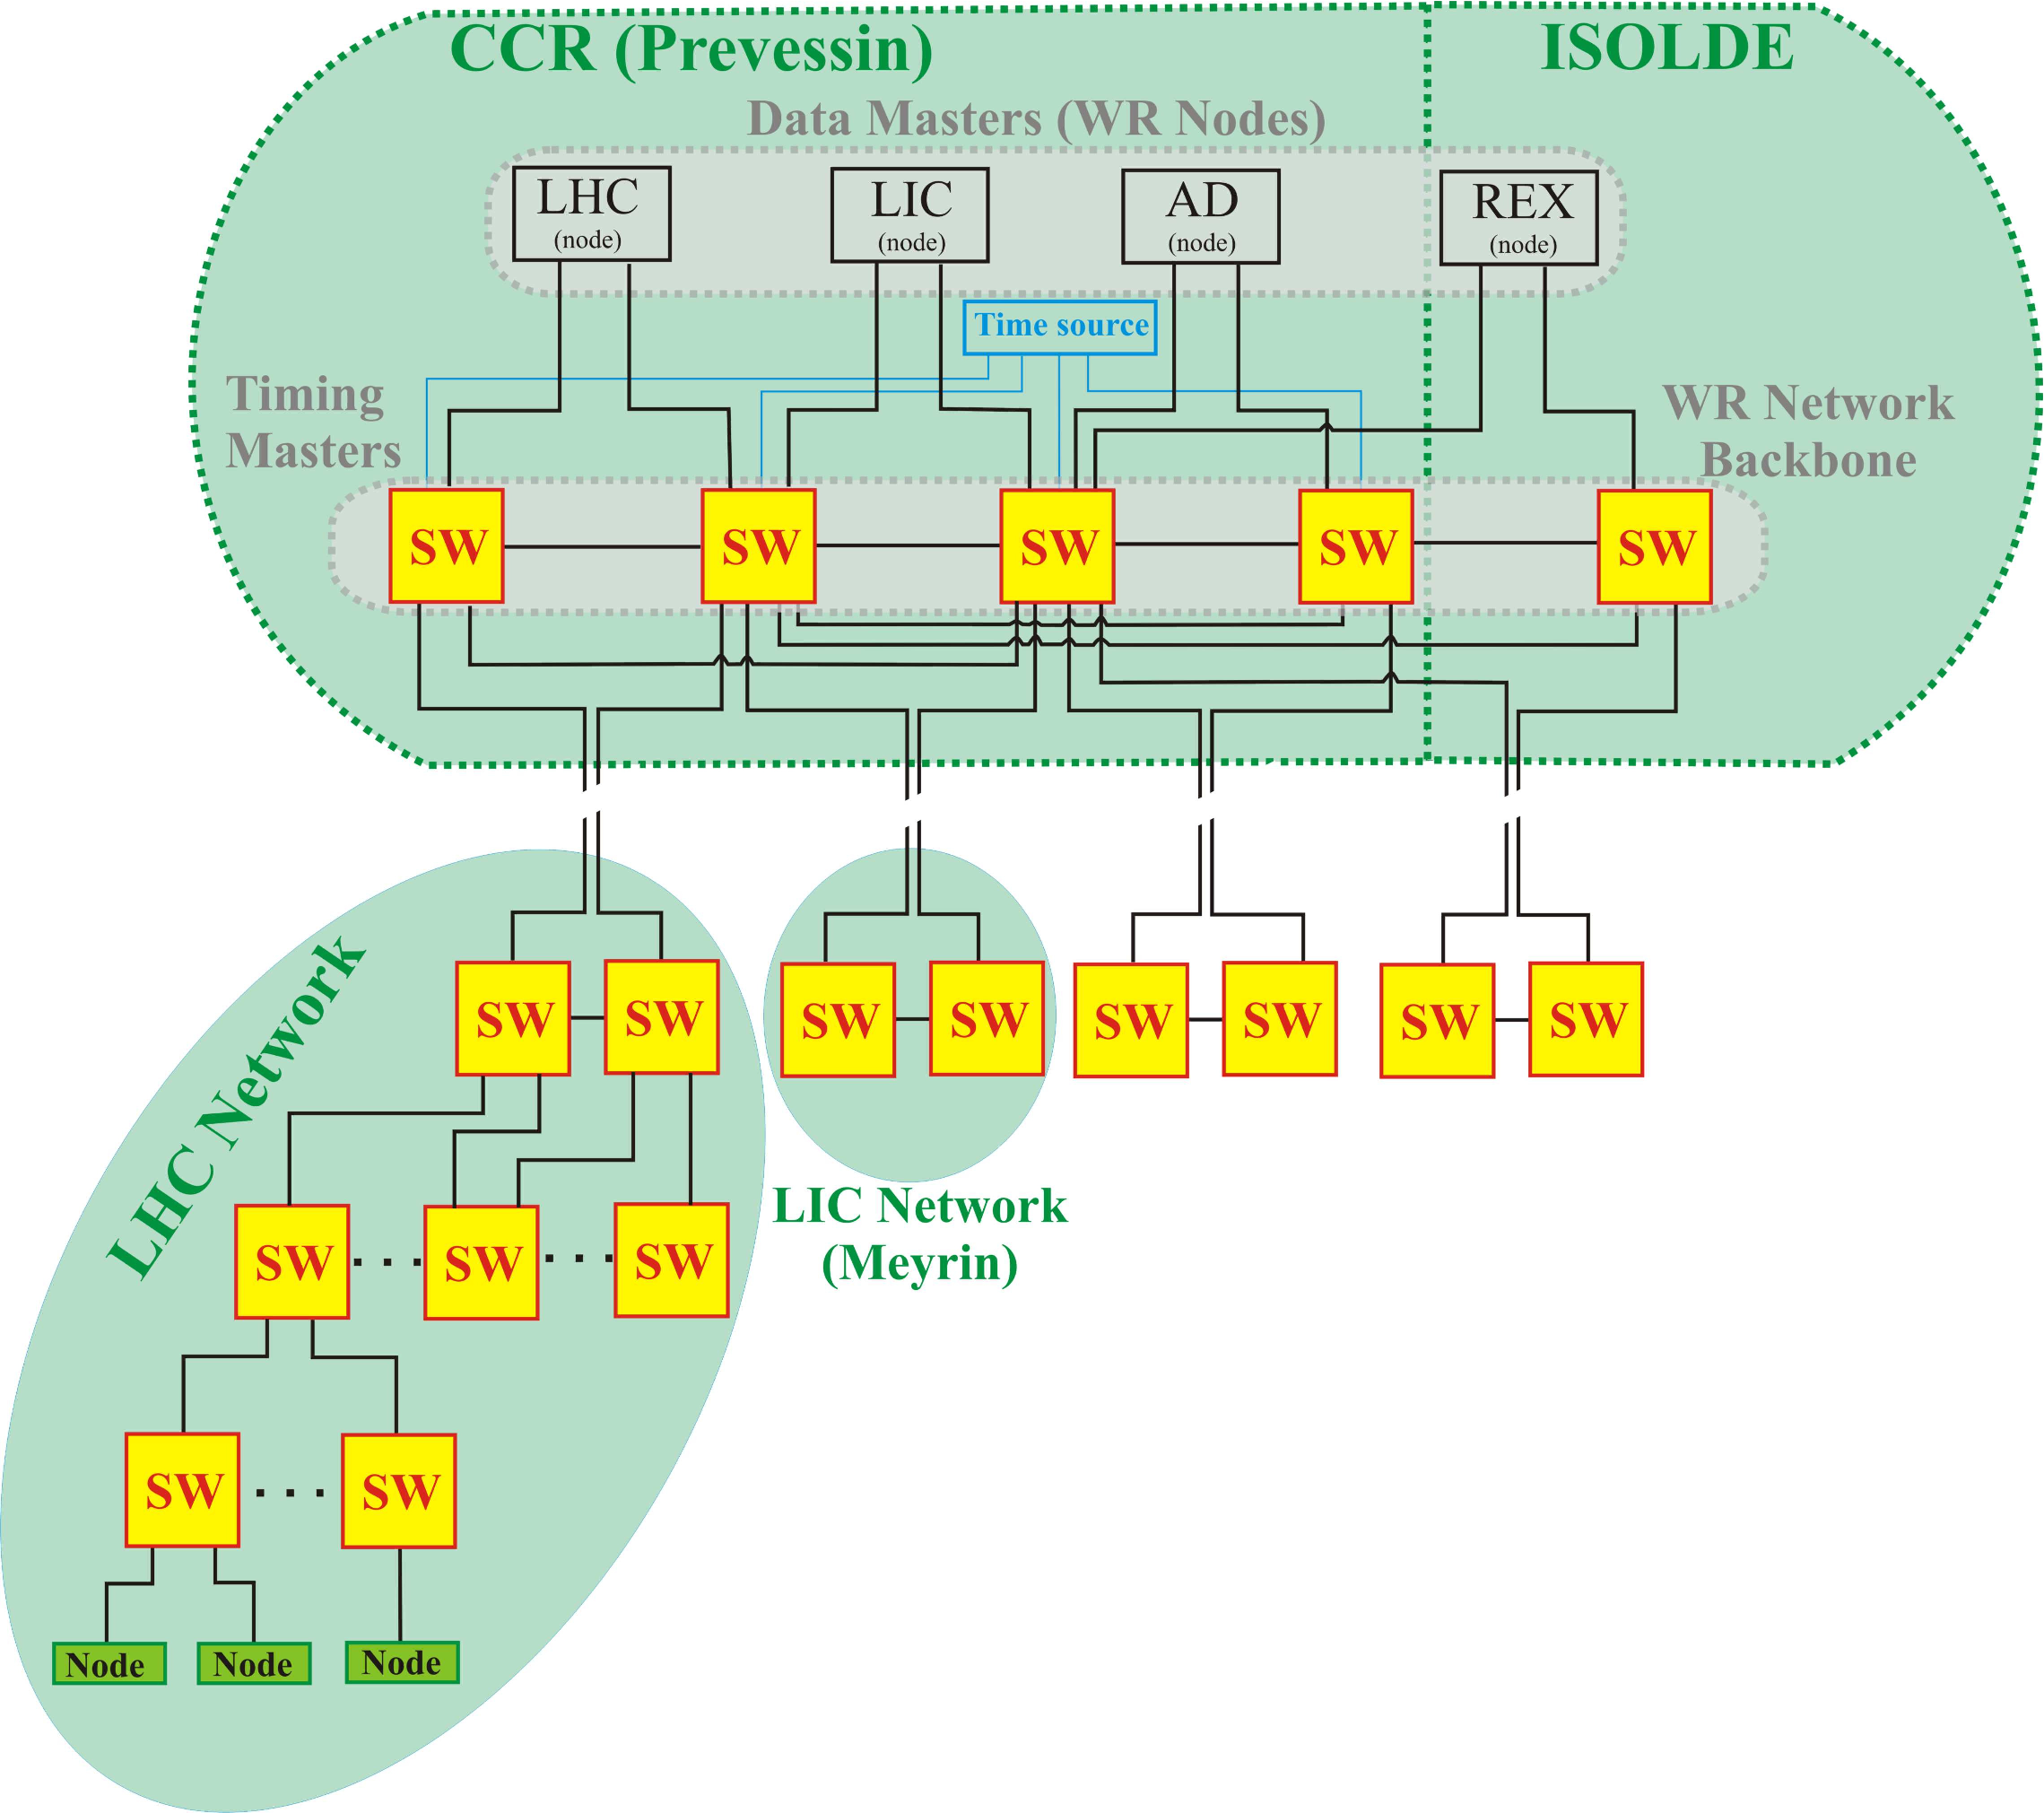
\includegraphics[width=.8\textwidth]{../../figures/applications/CERN/NT-overview.eps}
    \end{center}

\end{frame}
%%%%%%%%%%%%%%%%%%%%%%%%%%%%%%%%%%%%%%%%%%%%%%%%%%%%%%%%%%%%%%%%%%%%%%%%%%%%%%%%%%%%%%%%%%%%%%%%%%%%
%\section{Applications}
%\subsection{Topology Redundancy}
%%%%%%%%%%%%%%%%%%%%%%%%%%%%%%%%%%%%%%%%%%%%%%%%%%%%%%%%%%%%%%%%%%%%%%%%%%%%%%%%%%%%%%%%%%%%%%%%%%%%
\begin{frame}{Ethernet Clock Distribution a.k.a. Distributed DDS}
  \begin{center}
    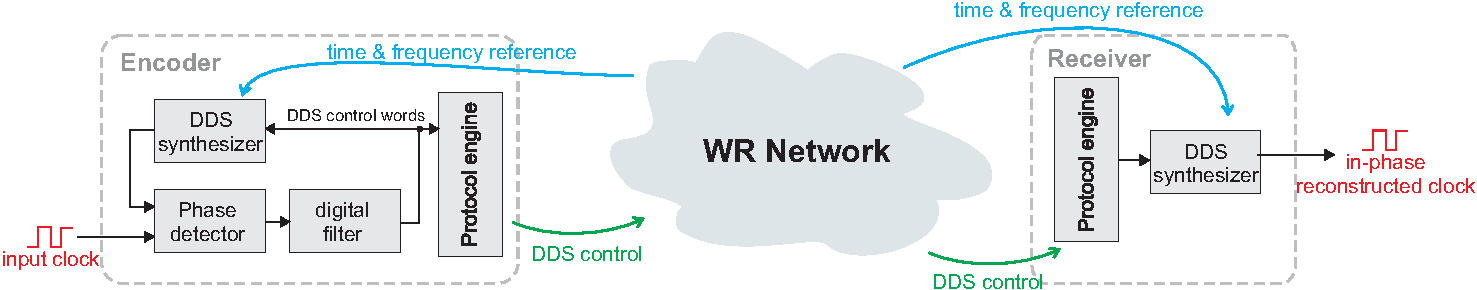
\includegraphics[width=\columnwidth]{../../figures/applications/remote_dds.eps}
  \end{center}
  \begin{block}{Distributed Direct Digital Synthesis}
    \begin{itemize}
    \item Replaces dozens of cables with a single fiber.
    \item Works over big distances without degrading signal quality.
    \item Can provide various clocks (e.g. RF, bunch clock) with a single, standardized link.
    \end{itemize}
  \end{block}
\end{frame}

%%%%%%%%%%%%%%%%%%%%%%%%%%%%%%%%%%%%%%%%%%%%%%%%%%%%%%%%%%%%%%%%%%%%%%%%%%%%%%%%%%%%%%%%%%%%%%%%%%%%
%\section{Applications}
%\subsection{Topology Redundancy}
%%%%%%%%%%%%%%%%%%%%%%%%%%%%%%%%%%%%%%%%%%%%%%%%%%%%%%%%%%%%%%%%%%%%%%%%%%%%%%%%%%%%%%%%%%%%%%%%%%%%
\begin{frame}{Distributed Oscilloscope}
  \begin{center}
    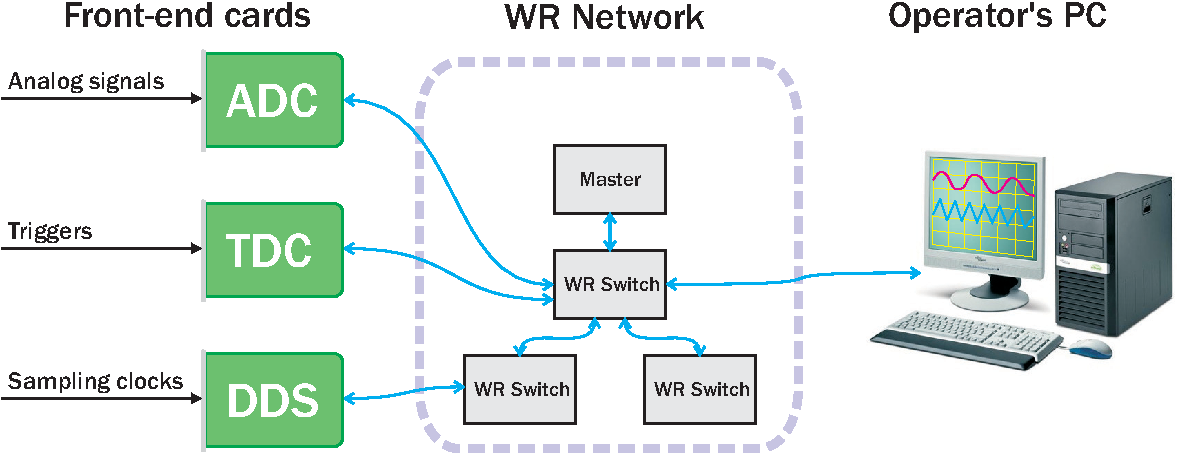
\includegraphics[width=0.9\textwidth]{../../figures/applications/distr_oscill.eps}
    \end{center}
    \begin{block}{}
      \begin{itemize}
      \item Common clock in the entire network: no skew between ADCs.
      \item Ability to sample with different clocks via Distributed DDS.
      \item External triggers can be time tagged with a TDC and used to reconstruct the original time base in the operator's PC.
      \end{itemize}
    \end{block}
\end{frame}
%%%%%%%%%%%%%%%%%%%%%%%%%%%%%%%%%%%%%%%%%%%%%%%%%%%%%%%%%%%%%%%%%%%%%%%%%%%%%%%%%%%%%%%%%%%%%%%%%%%%
%\section{Applications}
%\subsection{Topology Redundancy}
%%%%%%%%%%%%%%%%%%%%%%%%%%%%%%%%%%%%%%%%%%%%%%%%%%%%%%%%%%%%%%%%%%%%%%%%%%%%%%%%%%%%%%%%%%%%%%%%%%%%
\begin{frame}{CERN Neutrinos to Gran Sasso (CNGS)}

    \begin{center}
      \includegraphics[height=0.5\textheight]{figs/cngs-general.v2.eps} 
%       \includegraphics<2>[height=0.7\textheight]{figs/cngs-timing-3.eps}
    \end{center}

    \begin{center}
      \begin{itemize}
	\item Investigation of neutrino oscillation
	\item Time of Flight (ToF) measurement
      \end{itemize}

    \end{center}

\end{frame}
%%%%%%%%%%%%%%%%%%%%%%%%%%%%%%%%%%%%%%%%%%%%%%%%%%%%%%%%%%%%%%%%%%%%%%%%%%%%%%%%%%%%%%%%%%%%%%%%%%%%
%\section{Applications}
%\subsection{Topology Redundancy}
%%%%%%%%%%%%%%%%%%%%%%%%%%%%%%%%%%%%%%%%%%%%%%%%%%%%%%%%%%%%%%%%%%%%%%%%%%%%%%%%%%%%%%%%%%%%%%%%%%%%
\begin{frame}{CERN Neutrinos to Gran Sasso (CNGS)}

    \begin{center}
%       \includegraphics<1>[height=0.5\textheight]{figs/cngs-general.v2.eps} \pause
      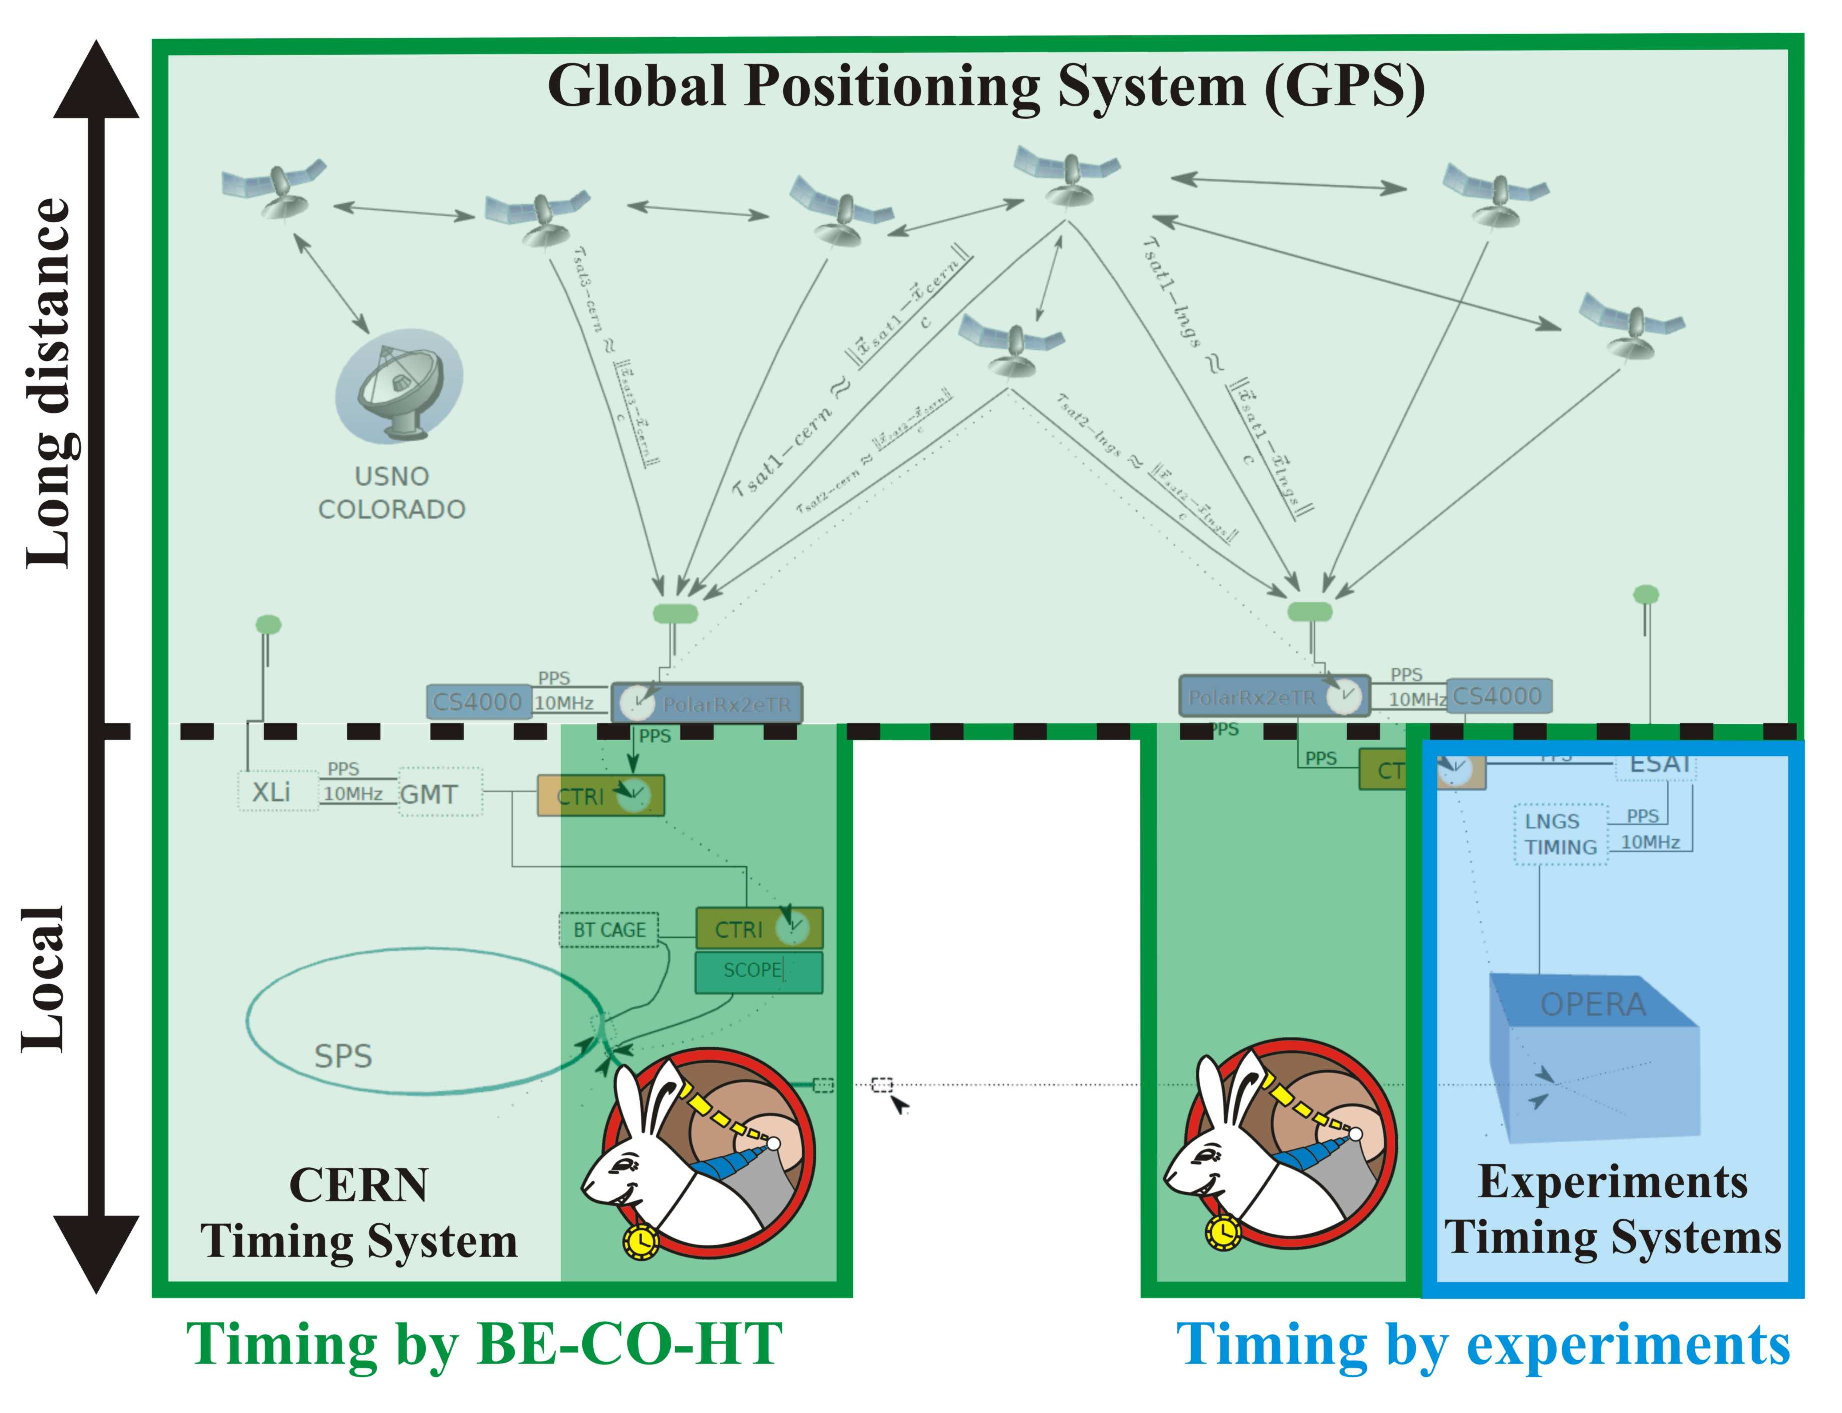
\includegraphics[height=0.7\textheight]{figs/cngs-timing-3.eps}
    \end{center}

    \begin{center}
      \begin{itemize}
	\item Investigation of neutrino oscillation
	\item Time of Flight (ToF) measurement
      \end{itemize}

    \end{center}


\end{frame}
%%%%%%%%%%%%%%%%%%%%%%%%%%%%%%%%%%%%%%%%%%%%%%%%%%%%%%%%%%%%%%%%%%%%%%%%%%%%%%%%%%%%%%%%%%%%%%%%%%%%
%\section{Applications}
%\subsection{Topology Redundancy}
%%%%%%%%%%%%%%%%%%%%%%%%%%%%%%%%%%%%%%%%%%%%%%%%%%%%%%%%%%%%%%%%%%%%%%%%%%%%%%%%%%%%%%%%%%%%%%%%%%%%
% 
% \begin{frame}{National Instruments}
% 
%     \begin{center}
%       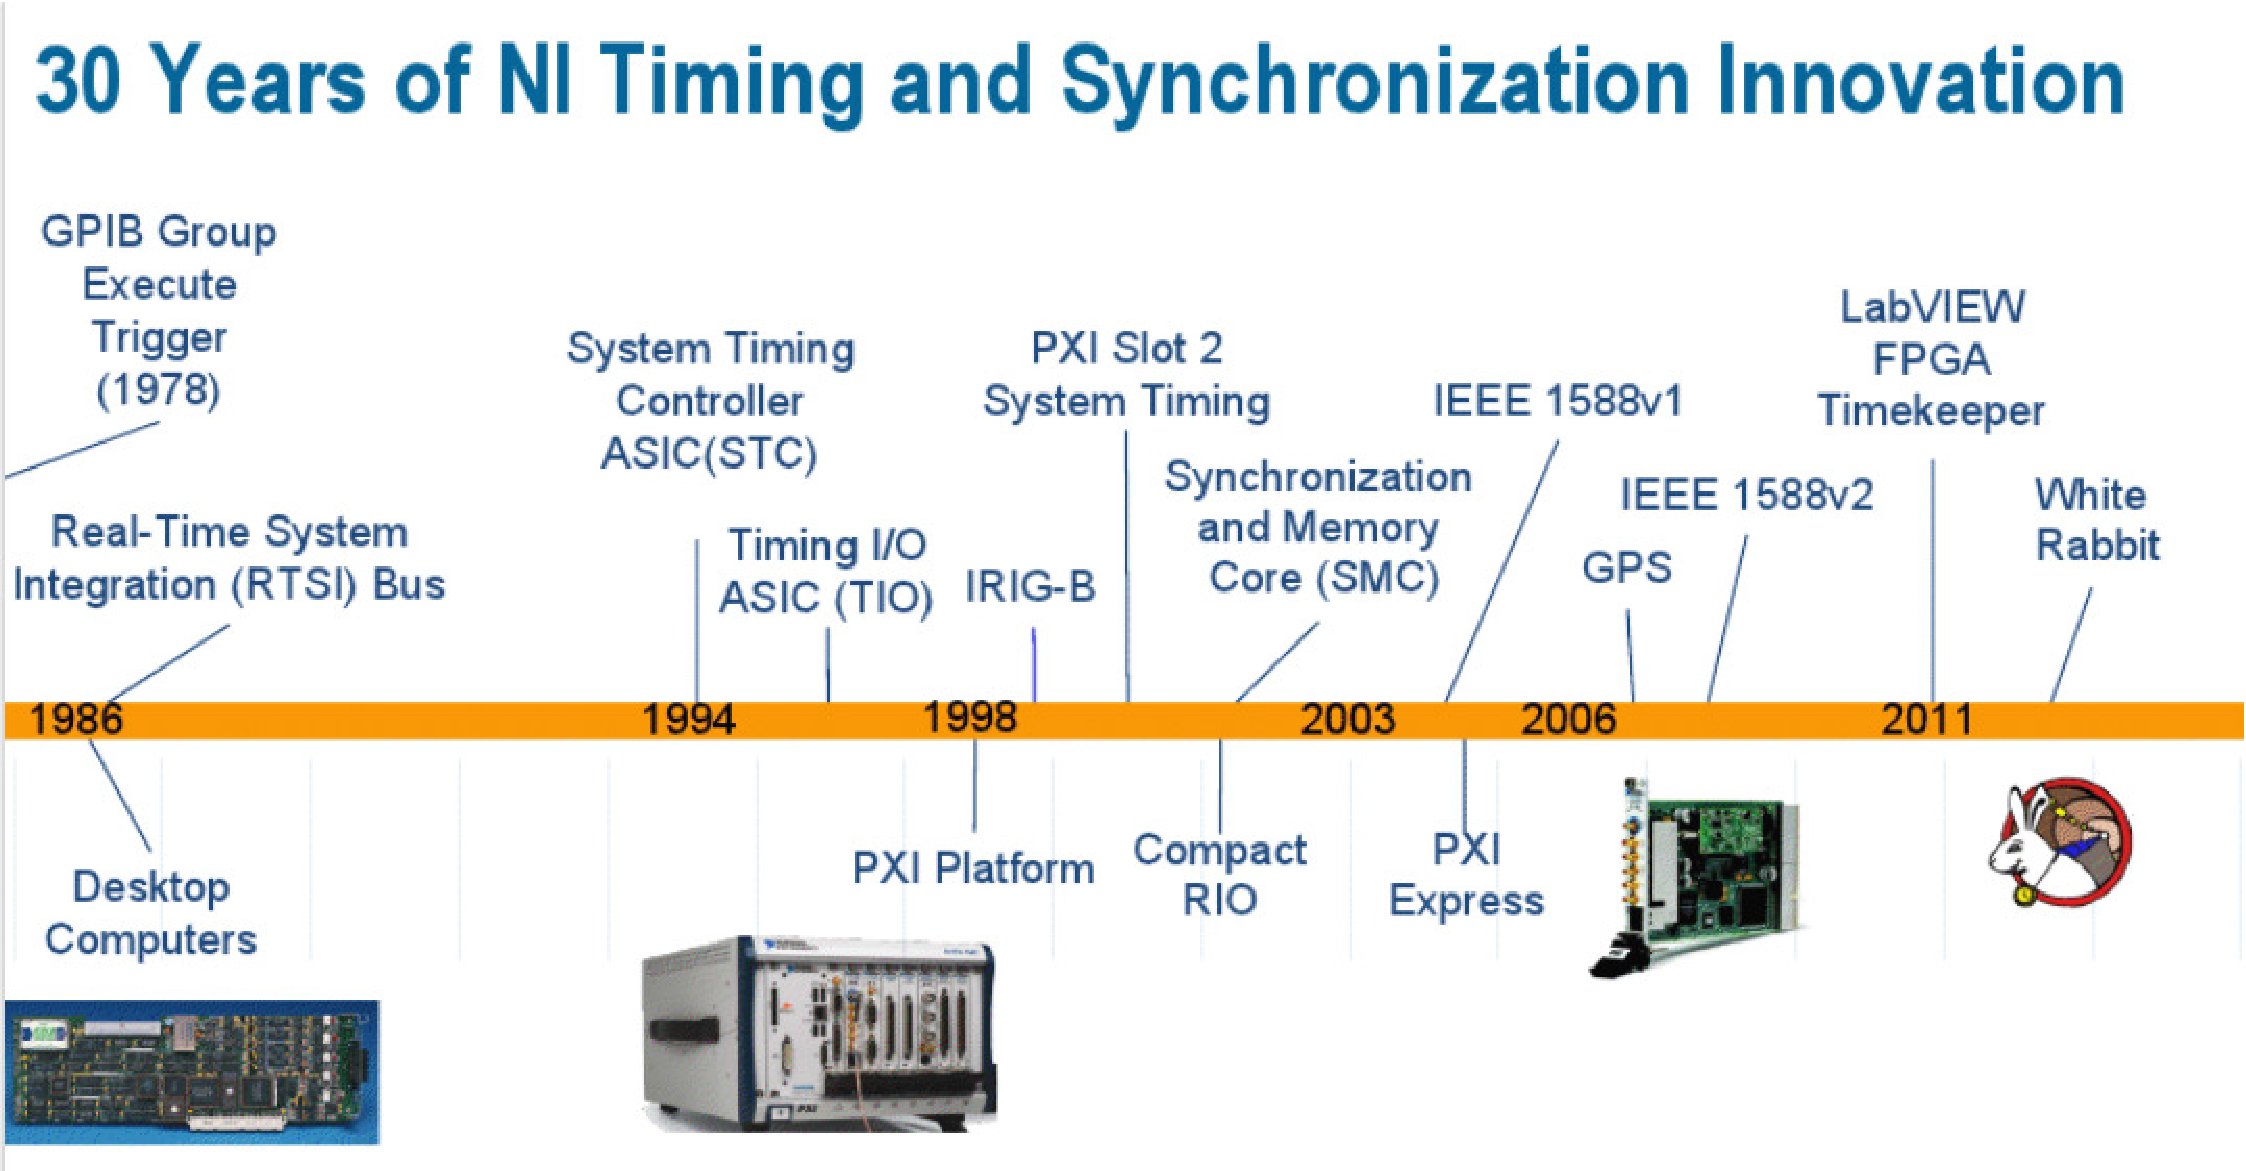
\includegraphics[width=1.0\textwidth]{../../figures/applications/ni.eps} 
%     \end{center}
% 
% \end{frame}
%%%%%%%%%%%%%%%%%%%%%%%%%%%%%%%%%%%%%%%%%%%%%%%%%%%%%%%%%%%%%%%%%%%%%%%%%%%%%%%%%%%%%%%%%%%%%%%%%%%%
%\section{Applications}
%\subsection{Topology Redundancy}
%%%%%%%%%%%%%%%%%%%%%%%%%%%%%%%%%%%%%%%%%%%%%%%%%%%%%%%%%%%%%%%%%%%%%%%%%%%%%%%%%%%%%%%%%%%%%%%%%%%%

\begin{frame}{Other White Rabbit Applications}

\begin{columns}[c]
  \column{0.65\textwidth}

    \begin{itemize}
      \item<1-> Future applications:
      \begin{itemize}
	\item<1-> \textbf<1>{GSI  }
	\item<2-> \textbf<2>{HiSCORE: Gamma\&Cosmic-Ray experiment (Tunka, Siberia)}
	\item<3-> \textbf<3>{The Large High Altitude Air Shower Observatory (China)}
      \end{itemize}         	
      \item<4-> Potential applications:
      \begin{itemize}
       \item<4-> \textbf<4>{SuperGPS through optical networks}
	\item<5-> \textbf<5>{Cherenkov Telescope Array}
	\item<6-> \textbf<6>{ITER}
	\item<7> \textbf<7>{European deep-sea research infrastructure (KM3NET)}
      \end{itemize}         	
    \end{itemize}    

  \column{0.55\textwidth}         


    \begin{center}
      \includegraphics<1>[width=0.85\textwidth]{figs/gsi.eps}   \pause
      \includegraphics<2>[width=0.85\textwidth]{../../figures/applications/tunka.eps}        \pause
      \includegraphics<3>[width=0.85\textwidth]{../../figures/applications/lhaaso.eps}       \pause
      \includegraphics<4>[width=0.85\textwidth]{figs/superGPS.eps}       \pause
      \includegraphics<5>[width=0.85\textwidth]{../../figures/applications/cta.eps}          \pause
      \includegraphics<6>[width=0.85\textwidth]{../../figures/applications/iter.eps}         \pause
      \includegraphics<7>[width=0.85\textwidth]{../../figures/applications/KM3NeT.eps}       
    \end{center}

  \column{0.6\textwidth}         
\end{columns}
\end{frame}
%%%%%%%%%%%%%%%%%%%%%%%%%%%%%%%%%%%%%%%%%%%%%%%%%%%%%%%%%%%%%%%%%%%%%%%%%%%%%%%%%%%%%%%%%%%%%%%%%%%%
\section{Performance}
\subsection{}
%%%%%%%%%%%%%%%%%%%%%%%%%%%%%%%%%%%%%%%%%%%%%%%%%%%%%%%%%%%%%%%%%%%%%%%%%%%%%%%%%%%%%%%%%%%%%%%%%%%%
\begin{frame}{WR time transfer performance: lab tests}

    \begin{center}
    \includegraphics<1>[height=7.0cm]{../../figures/measurements/measSystem.ps}   \pause
    \includegraphics<2>[height=6.0cm]{../../figures/measurements/measResults-new.eps}
    \end{center}

\end{frame}
%%%%%%%%%%%%%%%%%%%%%%%%%%%%%%%%%%%%%%%%%%%%%%%%%%%%%%%%%%%%%%%%%%%%%%%%%%%%%%%%%%%%%%%%%%%%%%%%%%%%
%\section{Status}
%\subsection{}
%%%%%%%%%%%%%%%%%%%%%%%%%%%%%%%%%%%%%%%%%%%%%%%%%%%%%%%%%%%%%%%%%%%%%%%%%%%%%%%%%%%%%%%%%%%%%%%%%%%%
\begin{frame}{WR Time Transfer Performance: CNGS Deployment}

  \begin{columns}[c]
	\column{0.6\textwidth}
	  \begin{center}

		\hspace{-1cm}
		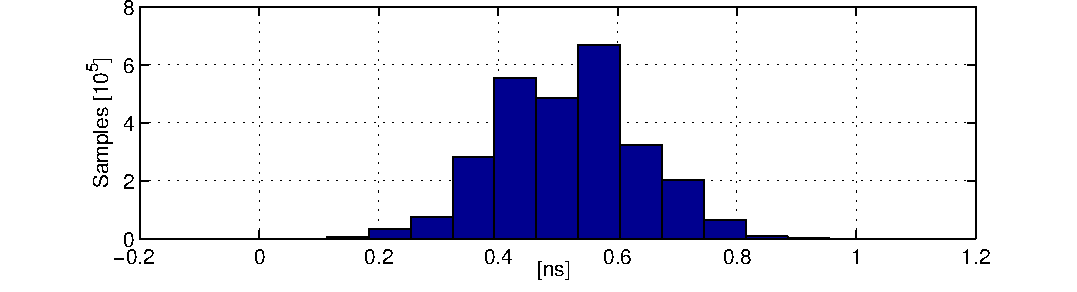
\includegraphics[width=1.1\textwidth]{../../figures/measurements/histogram-small.eps}
		\begin{itemize}
		       \item System performance
		       \begin{itemize}
		         	\item \textbf{Accuracy: 0.517 ns}
			      \item \textbf{Precision: 0.119 ns (std. dev)}
		\end{itemize}			  
		       \item Duration: 31 d, 7 h, 40 s ($2.7*10^6$ samples)
		       \item Timestamping reference PPS with 300 ps accuracy and 55 ps precision
		\end{itemize}			


	  \end{center}
	\column{0.6\textwidth}
		\begin{center}
		\includegraphics[width=0.93\textwidth]{../../figures/measurements/performance_testing_setup-detail.v2.eps}
		\end{center}
  \end{columns}
\end{frame}
%%%%%%%%%%%%%%%%%%%%%%%%%%%%%%%%%%%%%%%%%%%%%%%%%%%%%%%%%%%%%%%%%%%%%%%%%%%%%%%%%%%%%%%%%%%%%%%%%%%%
%\section{Status}
%\subsection{}
%%%%%%%%%%%%%%%%%%%%%%%%%%%%%%%%%%%%%%%%%%%%%%%%%%%%%%%%%%%%%%%%%%%%%%%%%%%%%%%%%%%%%%%%%%%%%%%%%%%%
\begin{frame}{WR Time Transfer Performance: CNGS Deployment}

  \begin{columns}[c]
	\column{0.6\textwidth}
	  \begin{center}

	    Out of $2.7*10^6$ samples\\
			\textbf{\textcolor{blue}{~9 values of $x_{diff}$ [0.0003$\%$]}} \\
                       exceeded MTIE=1ns
		


	  \end{center}
	\column{0.6\textwidth}
		\begin{center}
		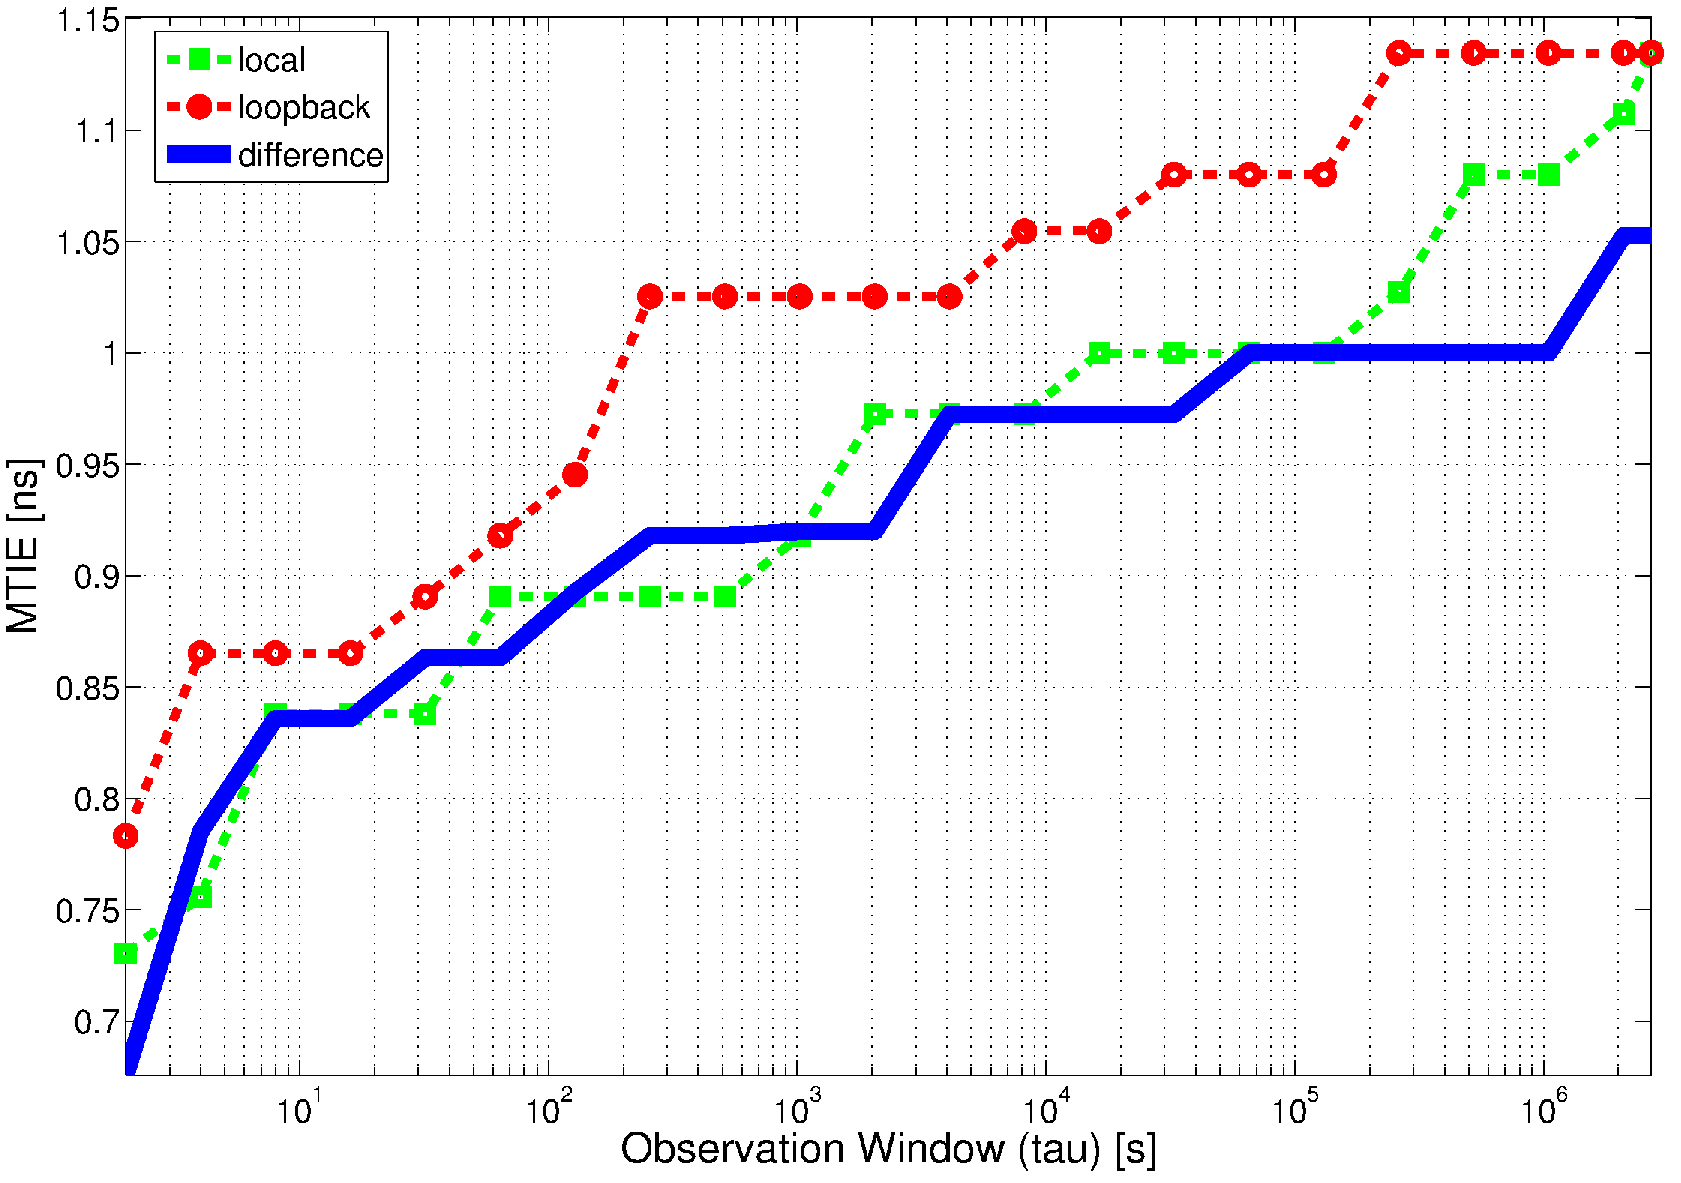
\includegraphics[width=0.9\textwidth]{../../figures/measurements/MTIE2.eps}
		\end{center}
  \end{columns}
\end{frame}


%%%%%%%%%%%%%%%%%%%%%%%%%%%%%%%%%%%%%%%%%%%%%%%%%%%%%%%%%%%%%%%%%%%%%%%%%%%%%%%%%%%%%%%%%%%%%%%%%%%%
\section{FIE and WR}
\subsection{}
%%%%%%%%%%%%%%%%%%%%%%%%%%%%%%%%%%%%%%%%%%%%%%%%%%%%%%%%%%%%%%%%%%%%%%%%%%%%%%%%%%%%%%%%%%%%%%%%%%%%
\begin{frame}{Future Internet Engineering and White Rabbit (1) }

\textbf{Future Internet Engineering}
    \begin{itemize}
      \item redefines/improves 3-7 OSI Layers
      \item uses newest solutions for 1-2 OSI Layers
      \item visualizes
    \end{itemize}    
\textbf{White Rabbit}
    \begin{itemize}
      \item improves 2 OSI Layer (i.e. GbE)
      \begin{itemize}
        \item high accuracy synchronization
        \item determinism
        \item reliability
      \end{itemize}    
      \item hardware-supports
    \end{itemize}    
\end{frame}
%%%%%%%%%%%%%%%%%%%%%%%%%%%%%%%%%%%%%%%%%%%%%%%%%%%%%%%%%%%%%%%%%%%%%%%%%%%%%%%%%%%%%%%%%%%%%%%%%%%%
% \section{FIE and WR}
% \subsection{}
%%%%%%%%%%%%%%%%%%%%%%%%%%%%%%%%%%%%%%%%%%%%%%%%%%%%%%%%%%%%%%%%%%%%%%%%%%%%%%%%%%%%%%%%%%%%%%%%%%%%
\begin{frame}{Future Internet Engineering and White Rabbit (2) }


	\textbf{Future Internet Engineering}
	  \begin{itemize}
		\item uses cutting edge Layer 2 equipment (e.g.: PIONIER)
		\item global scale: thousands of km with millions of nodes
		\item application: mass, public
	  \end{itemize}
	      \textbf{White Rabbit}
	  \begin{itemize}
		\item requires White Rabbit Layer 2 equipment
		\item large scale: tens of km with thousands of nodes
		\item application: dedicated, isolated, well-controlled
	  \end{itemize}

\end{frame}
%%%%%%%%%%%%%%%%%%%%%%%%%%%%%%%%%%%%%%%%%%%%%%%%%%%%%%%%%%%%%%%%%%%%%%%%%%%%%%%%%%%%%%%%%%%%%%%%%%%%
\section{Summary}
\subsection{}
%%%%%%%%%%%%%%%%%%%%%%%%%%%%%%%%%%%%%%%%%%%%%%%%%%%%%%%%%%%%%%%%%%%%%%%%%%%%%%%%%%%%%%%%%%%%%%%%%%%%
\begin{frame}{Summary}


    \begin{itemize}
      \item White Rabbit
      \begin{itemize}
	\item Thousands nodes
	\item $<$ 1ns accuracy
	\item determinism and reliability
	\item tested up to 10km
      \end{itemize}
      \item FIE and WR are complementary
      \item FIE is general-purpose and global-scale technology
      \item WR is specialized-purposed and large-scale technology
      \item WR improves the technology that FIE uses

    \end{itemize}    

 
\end{frame}
%%%%%%%%%%%%%%%%%%%%%%%%%%%%%%%%%%%%%%%%%%%%%%%%%%%%%%%%%%%%%%%%%%%%%%%%%%%%%%%%%%%%%%%%%%%%%%%%%%%%
%\section{Applications}
%\subsection{Topology Redundancy}
%%%%%%%%%%%%%%%%%%%%%%%%%%%%%%%%%%%%%%%%%%%%%%%%%%%%%%%%%%%%%%%%%%%%%%%%%%%%%%%%%%%%%%%%%%%%%%%%%%%%
% \begin{frame}{White Rabbits Family}
% \begin{columns}[c]
% \column{2.0in}
%     \begin{center}
%     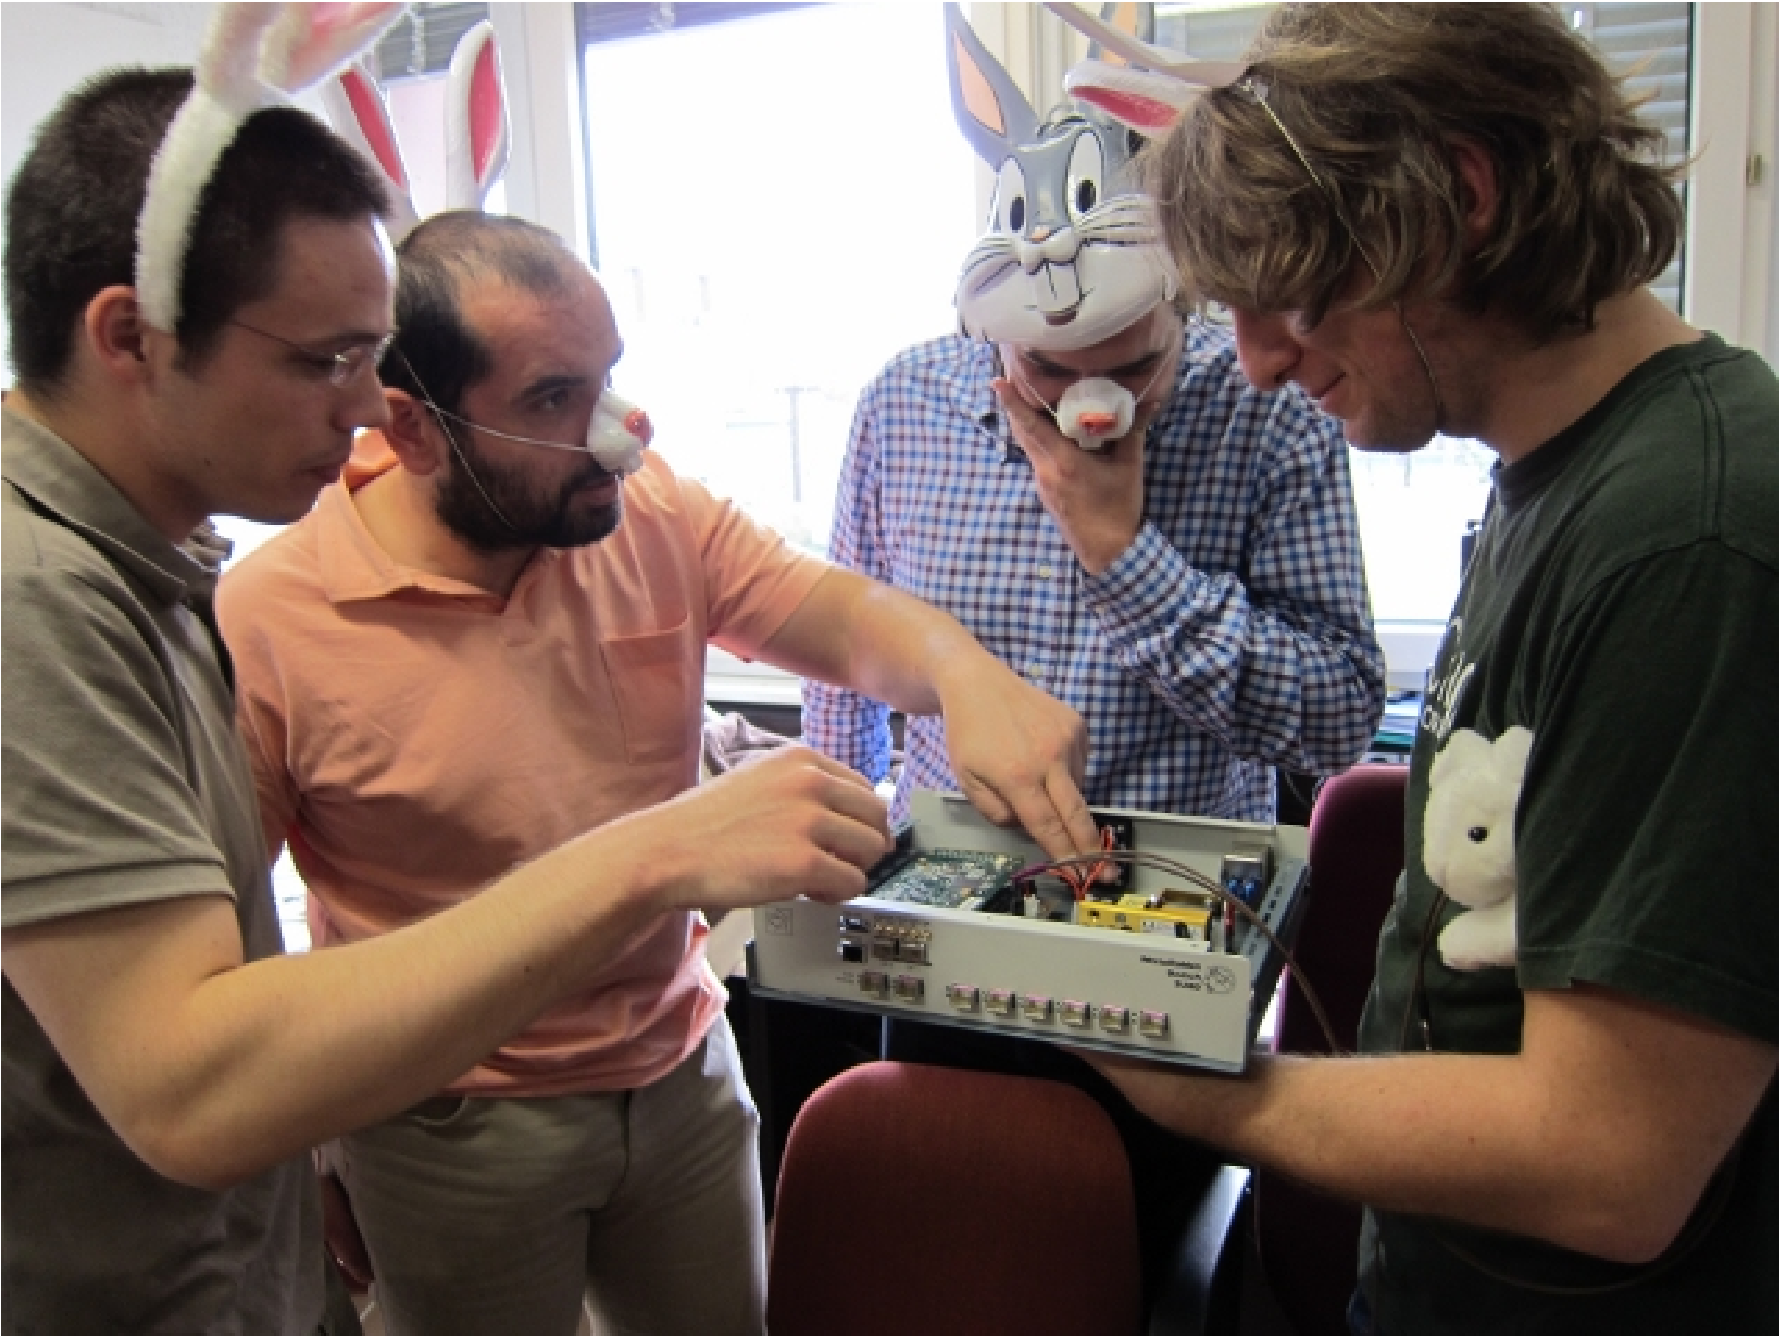
\includegraphics[width=3.5cm]{../../figures/misc/fourRabbits.ps}
%     \end{center}
% \column{2.0in}
%     \begin{center}
%     $\Leftarrow$ CERN geeks :) \\
%     All the family \\
%     $\Downarrow$
%      \end{center}
% \end{columns}
% 
% \begin{center}
% 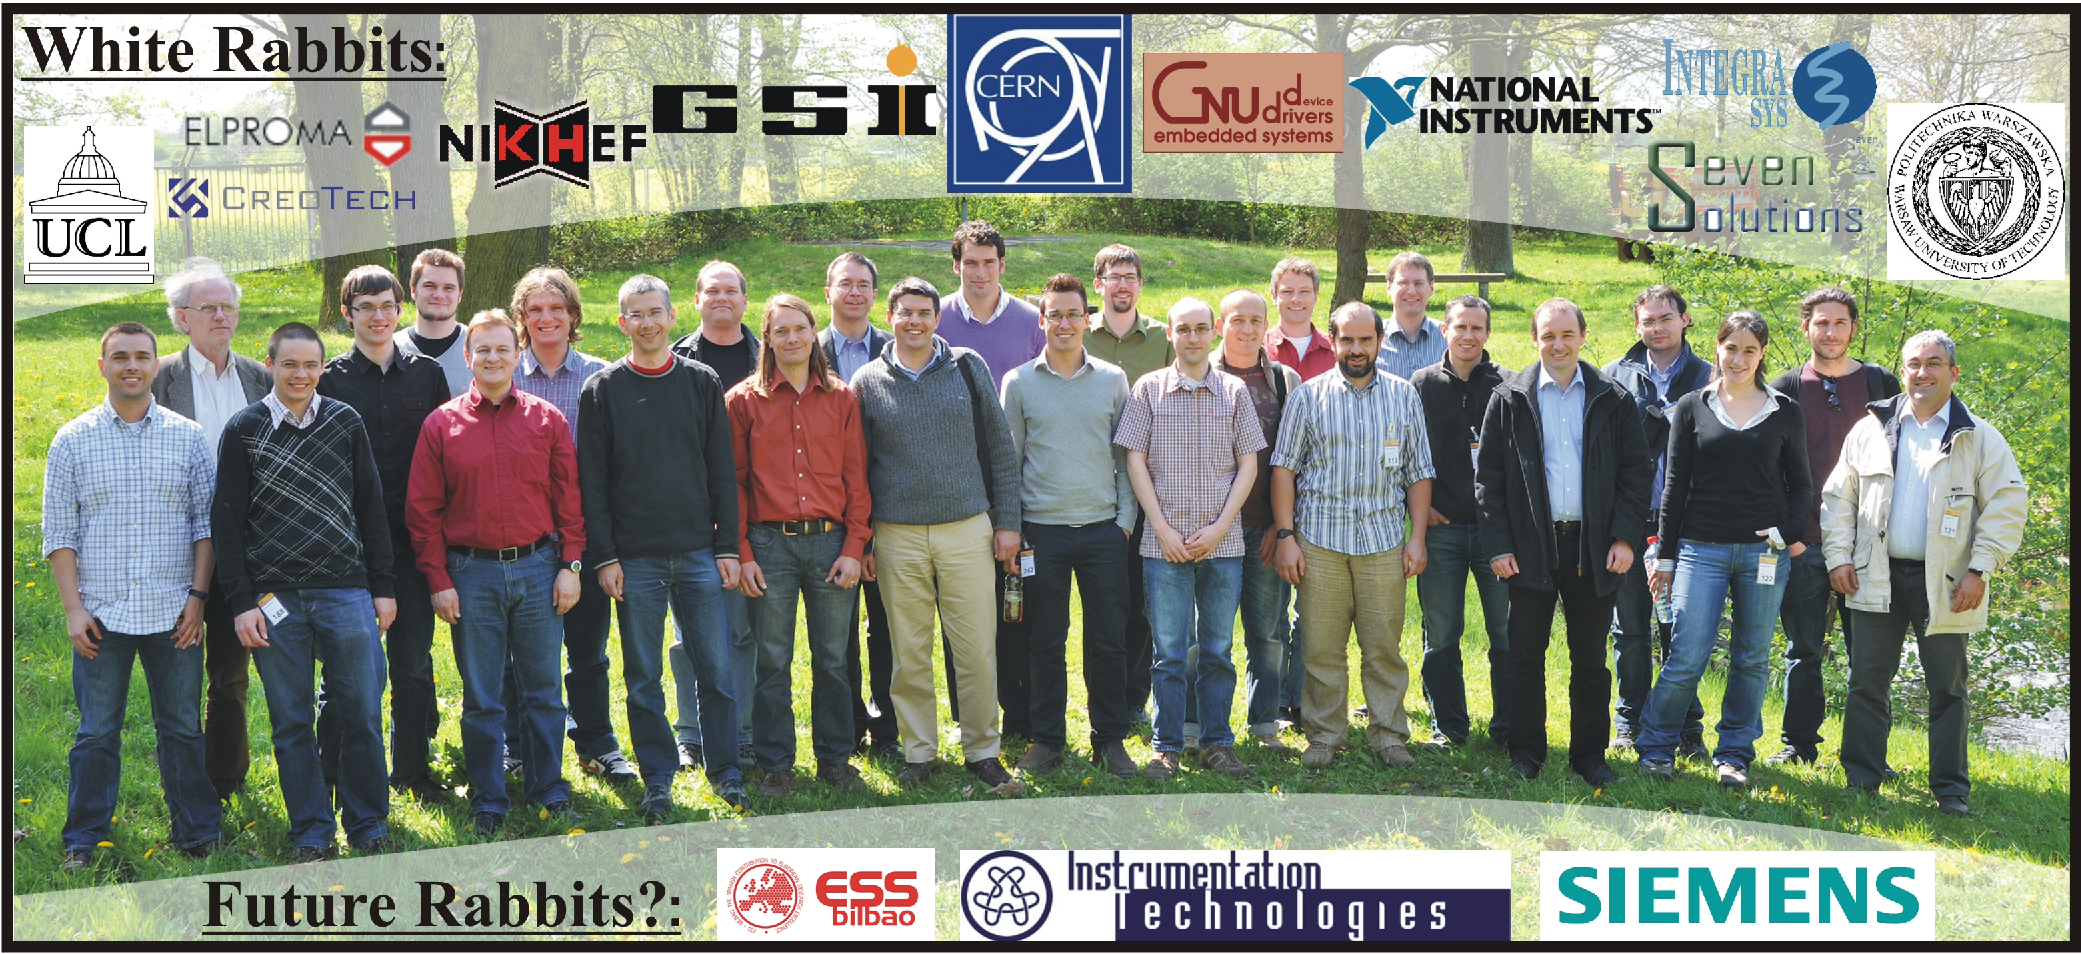
\includegraphics[width=9.5cm]{../../figures/misc/WRfamily.ps}
% \end{center}
% \end{frame}
%%%%%%%%%%%%%%%%%%%%%%%%%%%%%%%%%%%%%%%%%%%%%%%%%%%%%%%%%%%%%%%%%%%%%%%%%%%%%%%%%%%%%%%%%%%%%%%%%%%%
\section{Q\&A}
\subsection{}
%%%%%%%%%%%%%%%%%%%%%%%%%%%%%%%%%%%%%%%%%%%%%%%%%%%%%%%%%%%%%%%%%%%%%%%%%%%%%%%%%%%%%%%%%%%%%%%%%%%%
\begin{frame}{Questions and Answers}

    \begin{center}
    \includegraphics[height=4.0cm]{../../figures/logo/WRlogo.ps}
    \end{center}

\end{frame}

\appendix
\backupbegin


% %%%%%%%%%%%%%%%%%%%%%%%%%%%%%%%%%%%%%%%%%%%%%%%%%%%%%%%%%%%%%%%%%%%%%%%%%%%%%%%%%%%%%%%%%%%%%%%%%%%%
% %\section{Status}
% %\subsection{}
% %%%%%%%%%%%%%%%%%%%%%%%%%%%%%%%%%%%%%%%%%%%%%%%%%%%%%%%%%%%%%%%%%%%%%%%%%%%%%%%%%%%%%%%%%%%%%%%%%%%%
% \begin{frame}{WR performance}
% 
%     \begin{center}
%     \includegraphics<1>[height=7.0cm]{../../figures/measurements/measSystem.ps}   \pause
%     \includegraphics<2>[height=6.0cm]{../../figures/measurements/measResults-new.eps}
%     \end{center}
% 
% \end{frame}

%%%%%%%%%%%%%%%%%%%%%%%%%%%%%%%%%%%%%%%%%%%%%%%%%%%%%%%%%%%%%%%%%%%%%%%%%%%%%%%%%%%%%%%%%%%%%%%%%%%%
%\section{extras}
% \subsection{}
%%%%%%%%%%%%%%%%%%%%%%%%%%%%%%%%%%%%%%%%%%%%%%%%%%%%%%%%%%%%%%%%%%%%%%%%%%%%%%%%%%%%%%%%%%%%%%%%%%%%
\begin{frame}{Extras}

    \begin{center}
      Extras
    \end{center}

\end{frame}

%%%%%%%%%%%%%%%%%%%%%%%%%%%%%%%%%%%%%%%%%%%%%%%%%%%%%%%%%%%%%%%%%%%%%%%%%%%%%%%%%%%%%%%%%%%%%%%%%%%%
\section{CERN Control System}
\subsection{}
%%%%%%%%%%%%%%%%%%%%%%%%%%%%%%%%%%%%%%%%%%%%%%%%%%%%%%%%%%%%%%%%%%%%%%%%%%%%%%%%%%%%%%%%%%%%%%%%%%%%
\begin{frame}{CERN}

\begin{columns}[c]
  \column{0.55\textwidth}
    \begin{center}

      \begin{itemize}
	\item 6 accelerators
	\item LHC: 27km perimeter
	\item Thousands of devices to be controlled and synchronized
	\item A huge real-time distributed system
      \end{itemize}

    \end{center}
  \column{0.6\textwidth}
    \begin{center}
      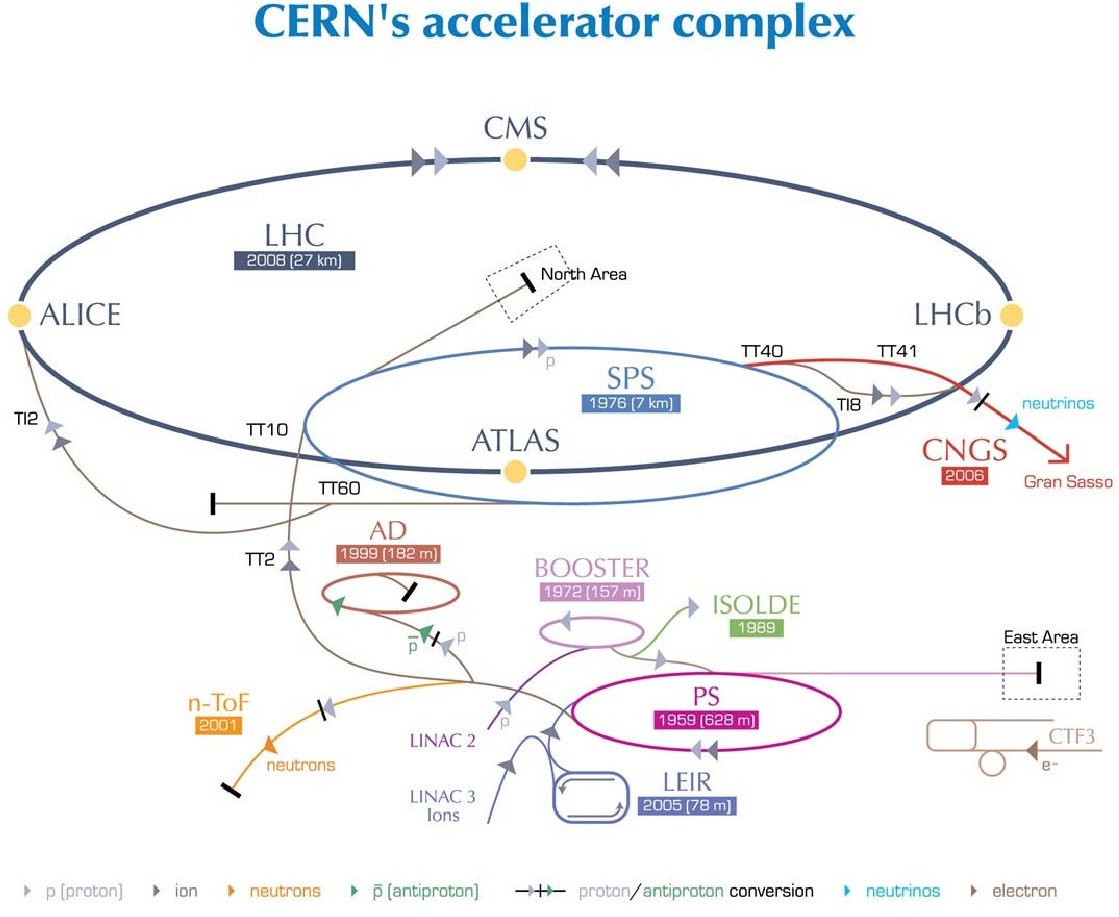
\includegraphics[width=6.5cm]{../../figures/applications/CERN/accelerators.eps}
    \end{center}
\end{columns}

\end{frame}
%%%%%%%%%%%%%%%%%%%%%%%%%%%%%%%%%%%%%%%%%%%%%%%%%%%%%%%%%%%%%%%%%%%%%%%%%%%%%%%%%%%%%%%%%%%%%%%%%%%%
% \section{}
% \subsection{}
%%%%%%%%%%%%%%%%%%%%%%%%%%%%%%%%%%%%%%%%%%%%%%%%%%%%%%%%%%%%%%%%%%%%%%%%%%%%%%%%%%%%%%%%%%%%%%%%%%%%
\begin{frame}{A Simplified Explanation of CERN Control System (1)}

      \begin{center}
      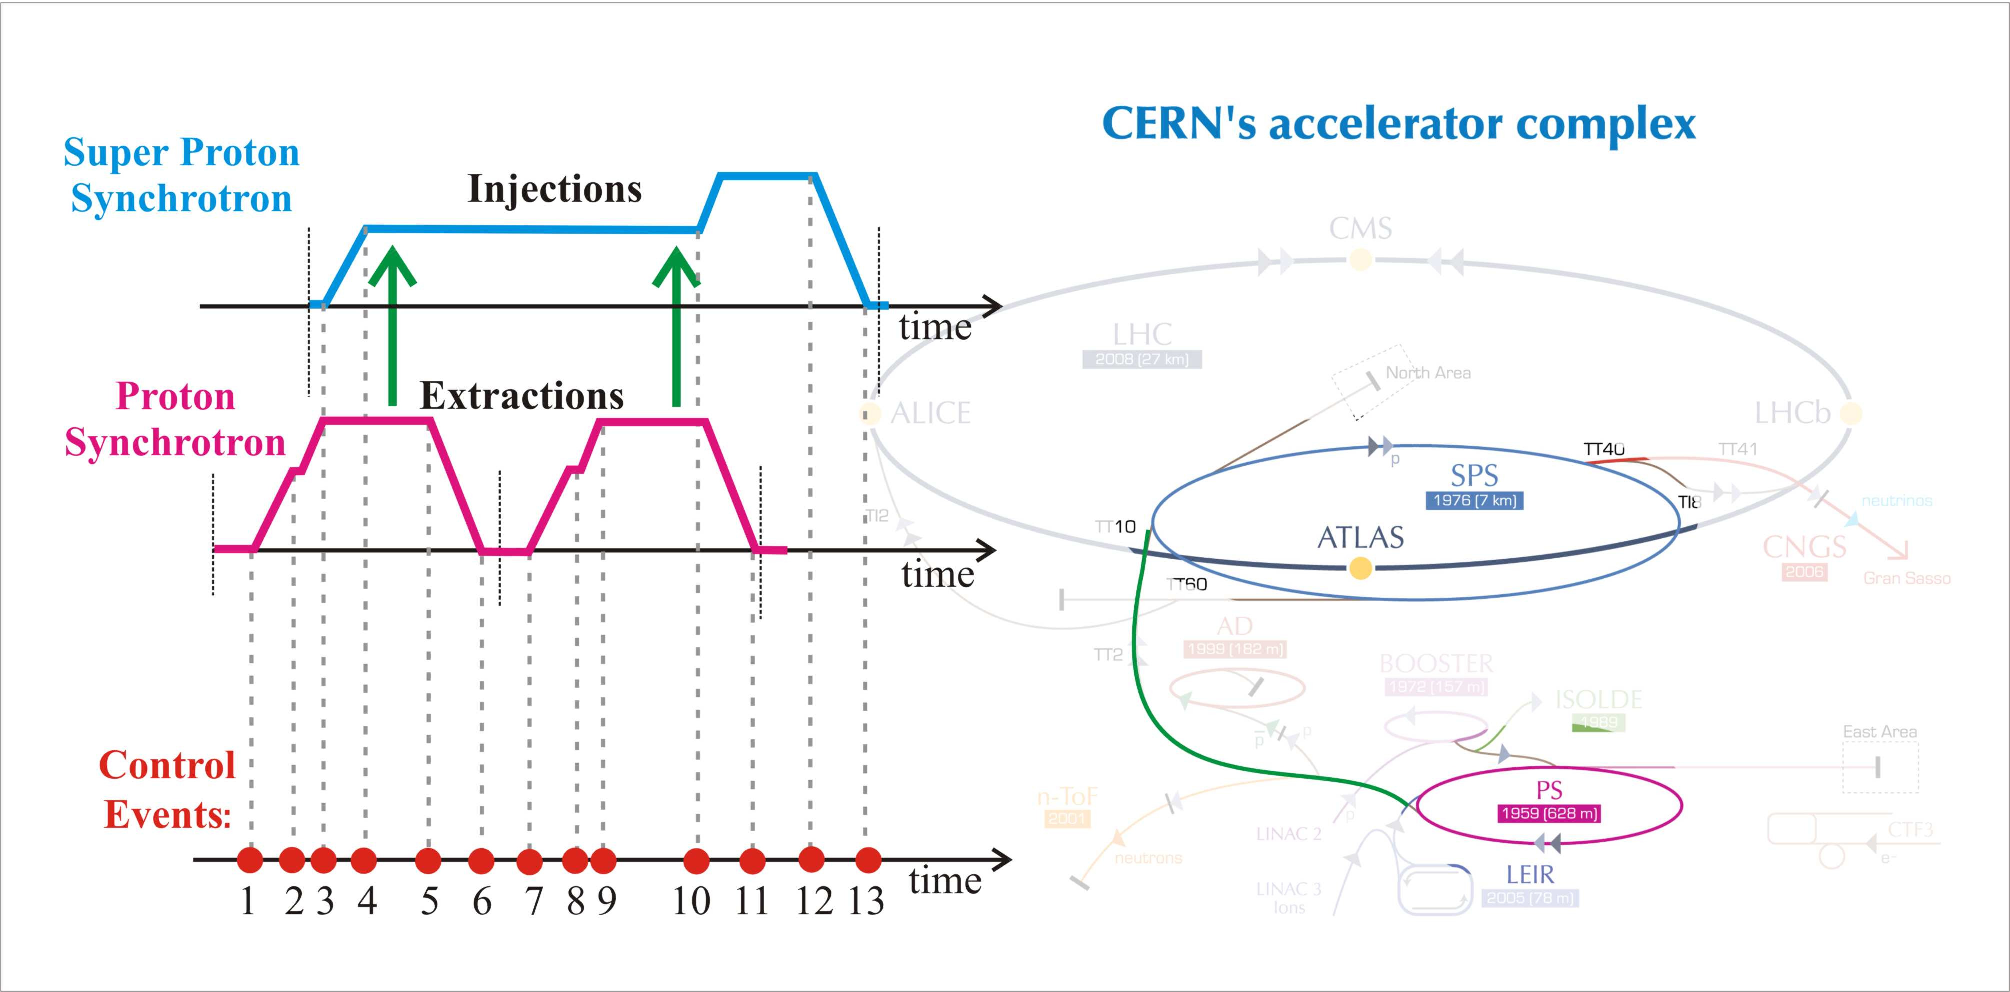
\includegraphics[width=1.0\textwidth]{../../figures/applications/CERN/event1.eps}
      \end{center}

  \begin{itemize}
    \item {\bf Events} -- points in time at which actions are triggered
    \item Each event is identified by an {\bf ID}
  \end{itemize}

\end{frame}


%%%%%%%%%%%%%%%%%%%%%%%%%%%%%%%%%%%%%%%%%%%%%%%%%%%%%%%%%%%%%%%%%%%%%%%%%%%%%%%%%%%%%%%%%%%%%%%%%%%%
% \section{}
% \subsection{}
%%%%%%%%%%%%%%%%%%%%%%%%%%%%%%%%%%%%%%%%%%%%%%%%%%%%%%%%%%%%%%%%%%%%%%%%%%%%%%%%%%%%%%%%%%%%%%%%%%%%
\begin{frame}{A Simplified Explanation of CERN Control System (2)}

      \begin{center}
      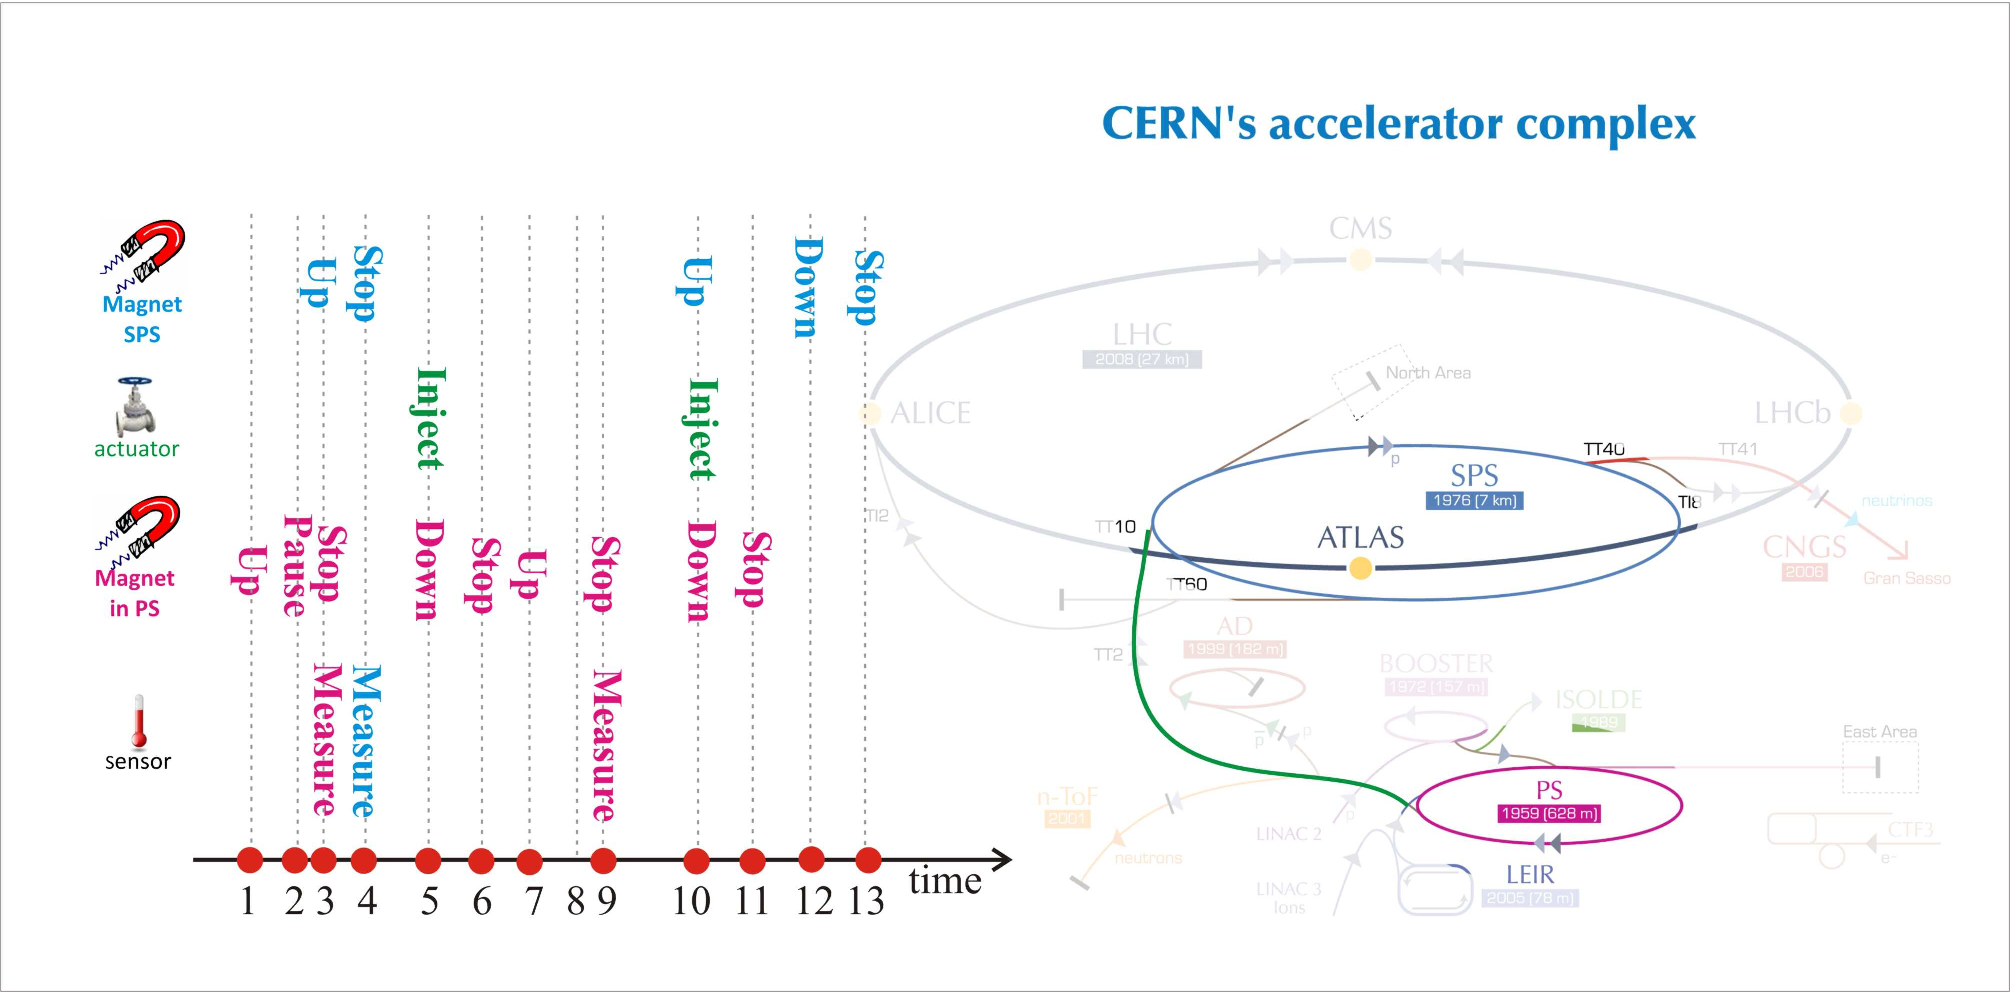
\includegraphics[width=1.0\textwidth]{../../figures/applications/CERN/event2.eps}
      \end{center}

  \begin{itemize}
    \item Devices are subscribed to events 
    \item Each device "knows" what to do on particular event
  \end{itemize}


\end{frame}


%%%%%%%%%%%%%%%%%%%%%%%%%%%%%%%%%%%%%%%%%%%%%%%%%%%%%%%%%%%%%%%%%%%%%%%%%%%%%%%%%%%%%%%%%%%%%%%%%%%%
% \section{}
% \subsection{}
%%%%%%%%%%%%%%%%%%%%%%%%%%%%%%%%%%%%%%%%%%%%%%%%%%%%%%%%%%%%%%%%%%%%%%%%%%%%%%%%%%%%%%%%%%%%%%%%%%%%
\begin{frame}{A Simplified Explanation of CERN Control System (3)}

      \begin{center}
      \includegraphics[width=.8\textwidth]{../../figures/applications/CERN/event3.eps}
      \end{center}

  \begin{itemize}
    \item Each event (ID) has a trigger time associated
	\item A set of events is sent as a single {\bf Control Message (CM)}
	\item CM is broadcast to all the end devices (nodes)
	\item CM is sent in advance ({\bf Granularity Window})
  \end{itemize}

\end{frame}

%%%%%%%%%%%%%%%%%%%%%%%%%%%%%%%%%%%%%%%%%%%%%%%%%%%%%%%%%%%%%%%%%%%%%%%%%%%%%%%%%%%%%%%%%%%%%%%%%%%%
% \section{}
% \subsection{}
%%%%%%%%%%%%%%%%%%%%%%%%%%%%%%%%%%%%%%%%%%%%%%%%%%%%%%%%%%%%%%%%%%%%%%%%%%%%%%%%%%%%%%%%%%%%%%%%%%%%
\begin{frame}{A Simplified Explanation of CERN Control System (4)}

\begin{columns}[c]
  \column{0.55\textwidth}
   {\bf Granuality Window: }
    \begin{center}
      \begin{itemize}
	    \item Controller-input to node-output (i.e. pulse)
	    \item Maximum bound latency {\bf guaranteed } by the system
	    \item Processing and network latency included
      \end{itemize}

    \end{center}
  \column{0.6\textwidth}
    \begin{center}
      \begin{center}
      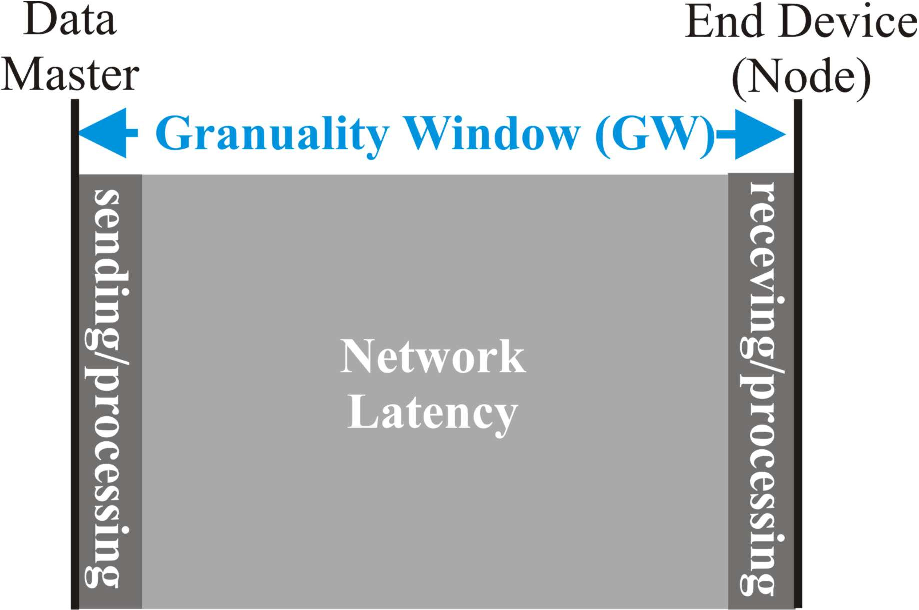
\includegraphics[width=.8\textwidth]{../../figures/applications/CERN/gw.eps}
      \end{center}
    \end{center}
\end{columns}

\end{frame}

%%%%%%%%%%%%%%%%%%%%%%%%%%%%%%%%%%%%%%%%%%%%%%%%%%%%%%%%%%%%%%%%%%%%%%%%%%%%%%%%%%%%%%%%%%%%%%%%%%%%
% \section{}
% \subsection{}
%%%%%%%%%%%%%%%%%%%%%%%%%%%%%%%%%%%%%%%%%%%%%%%%%%%%%%%%%%%%%%%%%%%%%%%%%%%%%%%%%%%%%%%%%%%%%%%%%%%%
% \begin{frame}{A simplified explanation of CERN control system (5)}
% 
%       \begin{center}
%       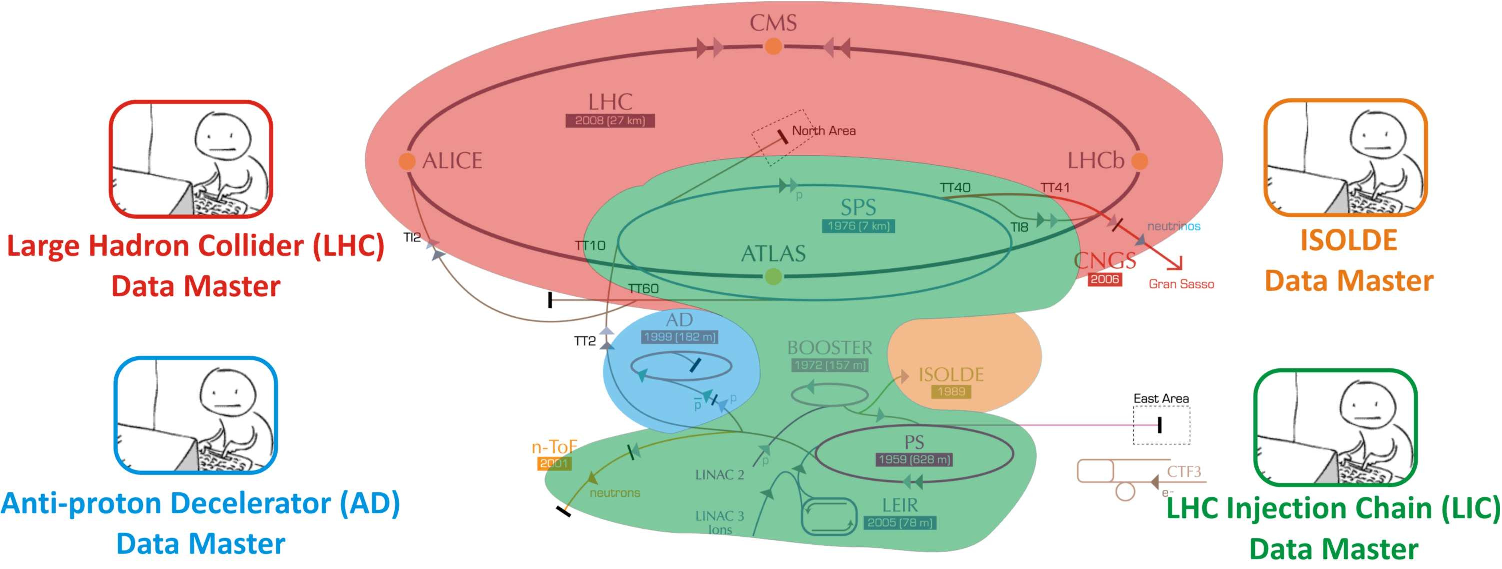
\includegraphics[width=.7\textwidth]{../../figures/applications/CERN/accNetworks.eps}
%       \end{center}
% 
%   \begin{itemize}
%     \item 4 accelerator networks
%     \item Separate {\bf Data Master (DM)} for each network
%     \item \textcolor{green!90}{LIC Data Master} communicates with other DMs and control devices in their networks
%     \item Broadcast of {\bf Control Messages} within network(s)
%   \end{itemize}
% 
% \end{frame}

%%%%%%%%%%%%%%%%%%%%%%%%%%%%%%%%%%%%%%%%%%%%%%%%%%%%%%%%%%%%%%%%%%%%%%%%%%%%%%%%%%%%%%%%%%%%%%%%%%%%
% \subsection{}
%%%%%%%%%%%%%%%%%%%%%%%%%%%%%%%%%%%%%%%%%%%%%%%%%%%%%%%%%%%%%%%%%%%%%%%%%%%%%%%%%%%%%%%%%%%%%%%%%%%%
\begin{frame}{Time Distribution in White Rabbit}

  \begin{itemize}
    \item Synchronization with {\bf sub-ns} accuracy over fiber
    \item Combination of
	\begin{itemize}
	  \item Precision Time Protocol ({\bf PTP}) synchronization
	  \item Synchronous Ethernet ({\bf SyncE}) syntonization
	  \item Digital Dual-Mixer Time Difference ({\bf DDMTD}) phase detection
	\end{itemize}
%    \item Reliability-oriented.
    \item WR Link:
  \end{itemize}

  \begin{center}
  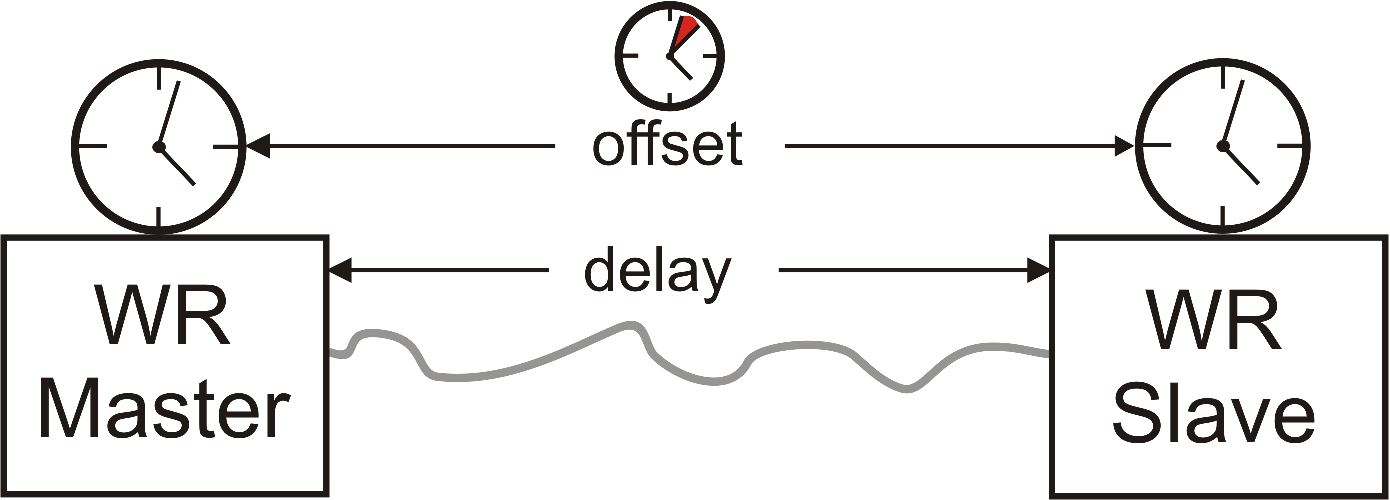
\includegraphics[height=3cm]{../../figures/protocol/wrLink.ps}
  \end{center}

\end{frame}

%%%%%%%%%%%%%%%%%%%%%%%%%%%%%%%%%%%%%%%%%%%%%%%%%%%%%%%%%%%%%%%%%%%%%%%%%%%%%%%%%%%%%%%%%%%%%%%%%%%%
%\section{Timestamps}
\subsection{}
%%%%%%%%%%%%%%%%%%%%%%%%%%%%%%%%%%%%%%%%%%%%%%%%%%%%%%%%%%%%%%%%%%%%%%%%%%%%%%%%%%%%%%%%%%%%%%%%%%%%
\begin{frame}{Fine Delay Measurement}

  \begin{center}
  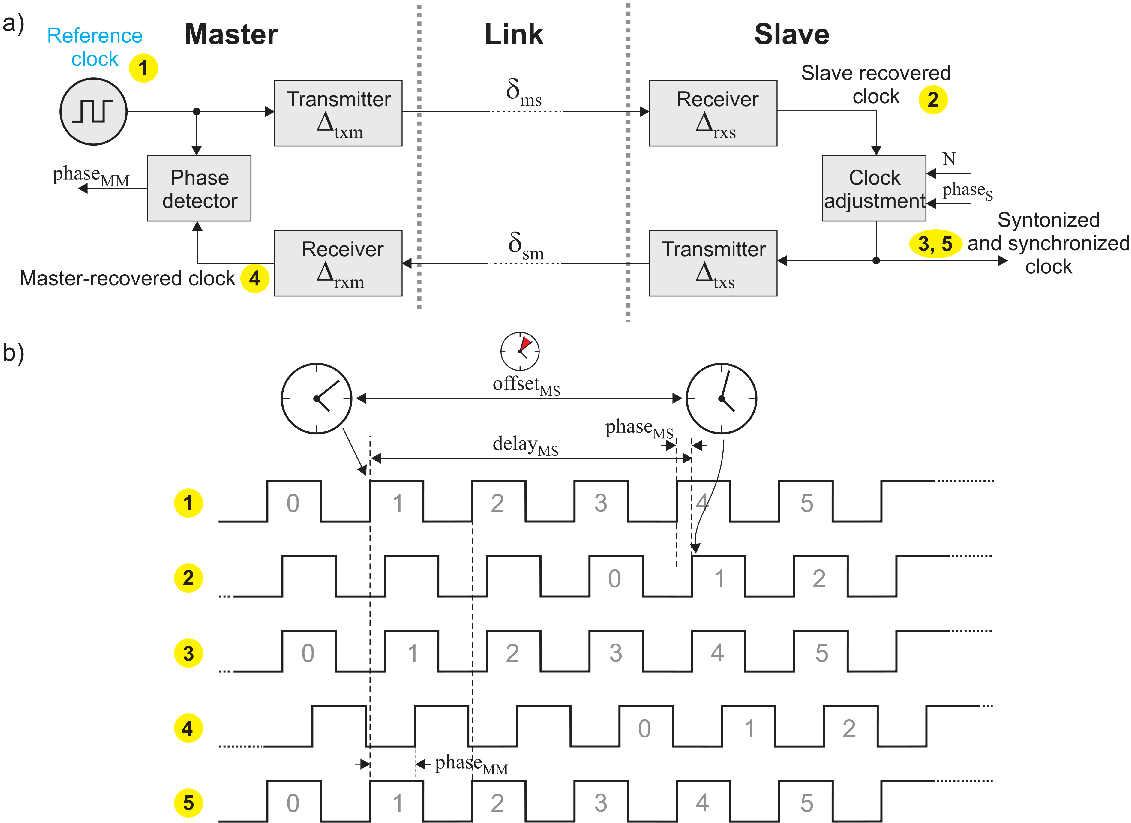
\includegraphics[width=10.0cm]{../../figures/protocol/link_model.eps}
  \end{center}

\end{frame}

%%%%%%%%%%%%%%%%%%%%%%%%%%%%%%%%%%%%%%%%%%%%%%%%%%%%%%%%%%%%%%%%%%%%%%%%%%%%%%%%%%%%%%%%%%%%%%%%%%%%
%\section{Link Delay Model}
%\subsection{}
%%%%%%%%%%%%%%%%%%%%%%%%%%%%%%%%%%%%%%%%%%%%%%%%%%%%%%%%%%%%%%%%%%%%%%%%%%%%%%%%%%%%%%%%%%%%%%%%%%%%
\begin{frame}{Link Delay Model}

  \begin{align}
    \nonumber delay_{ms} &= \Delta_{tx_m} + \delta_{ms} + \Delta_{rx_s} \\
    \nonumber delay_{sm} &= \Delta_{tx_s} + \delta_{sm} + \Delta_{rx_m}
  \end{align}

   \vspace{0.2cm}

  \begin{center}
  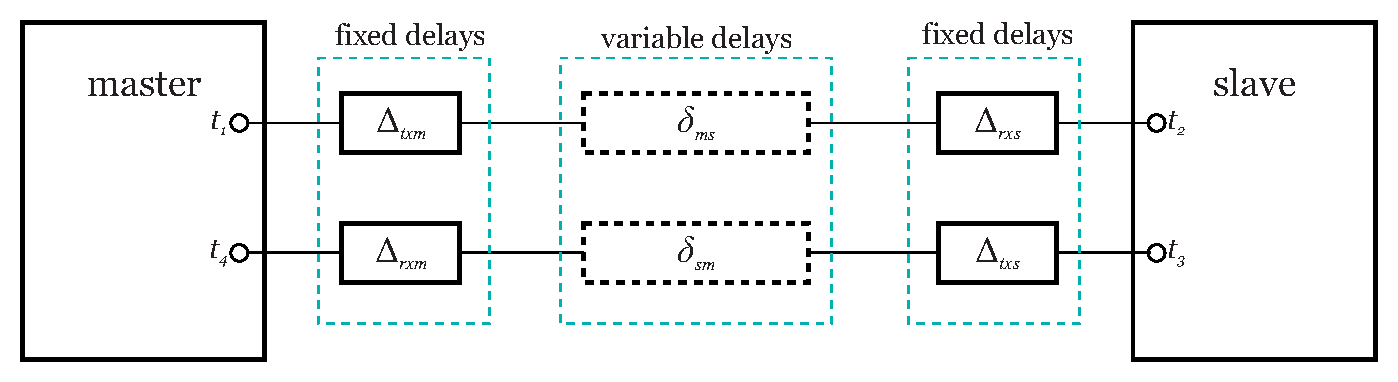
\includegraphics[height=2.5cm]{../../figures/protocol/delaymodel.eps}
  \end{center}

\begin{columns}[c]
  \column{2.8in}

    \begin{center}
      \textbf{Relative Delay Coefficient ($\alpha$)} \\
      for 1000BASE-BX10 over a Single-mode Optical Fiber
    \end{center}

  \column{1.5in}
    \begin{center}
      \begin{equation}
      \nonumber \delta_{ms} = (1 + \alpha) \, \delta_{sm}
      \end{equation}
    \end{center}
    \vspace{0.5cm}
\end{columns}
  
\end{frame}

%%%%%%%%%%%%%%%%%%%%%%%%%%%%%%%%%%%%%%%%%%%%%%%%%%%%%%%%%%%%%%%%%%%%%%%%%%%%%%%%%%%%%%%%%%%%%%%%%%%%
%\section{Link Delay Model}
% \subsection{}
%%%%%%%%%%%%%%%%%%%%%%%%%%%%%%%%%%%%%%%%%%%%%%%%%%%%%%%%%%%%%%%%%%%%%%%%%%%%%%%%%%%%%%%%%%%%%%%%%%%%
\begin{frame}{Fixed Delays}

  \begin{center}
  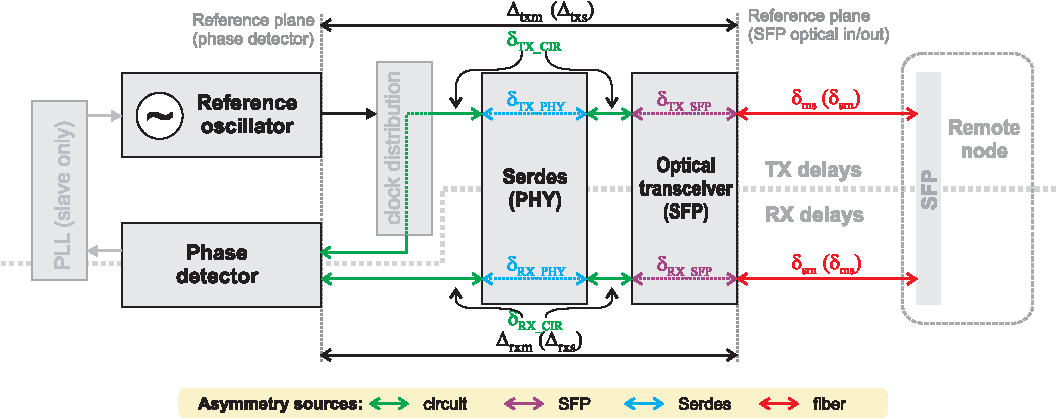
\includegraphics[width=11.0cm]{../../figures/protocol/asymmetries.eps}
  \end{center}

\end{frame}


%%%%%%%%%%%%%%%%%%%%%%%%%%%%%%%%%%%%%%%%%%%%%%%%%%%%%%%%%%%%%%%%%%%%%%%%%%%%%%%%%%%%%%%%%%%%%%%%%%%%
%\section{Link Asymmetry}
% \subsection{}
%%%%%%%%%%%%%%%%%%%%%%%%%%%%%%%%%%%%%%%%%%%%%%%%%%%%%%%%%%%%%%%%%%%%%%%%%%%%%%%%%%%%%%%%%%%%%%%%%%%%
\begin{frame}{Link Asymmetry}

  \begin{center}
  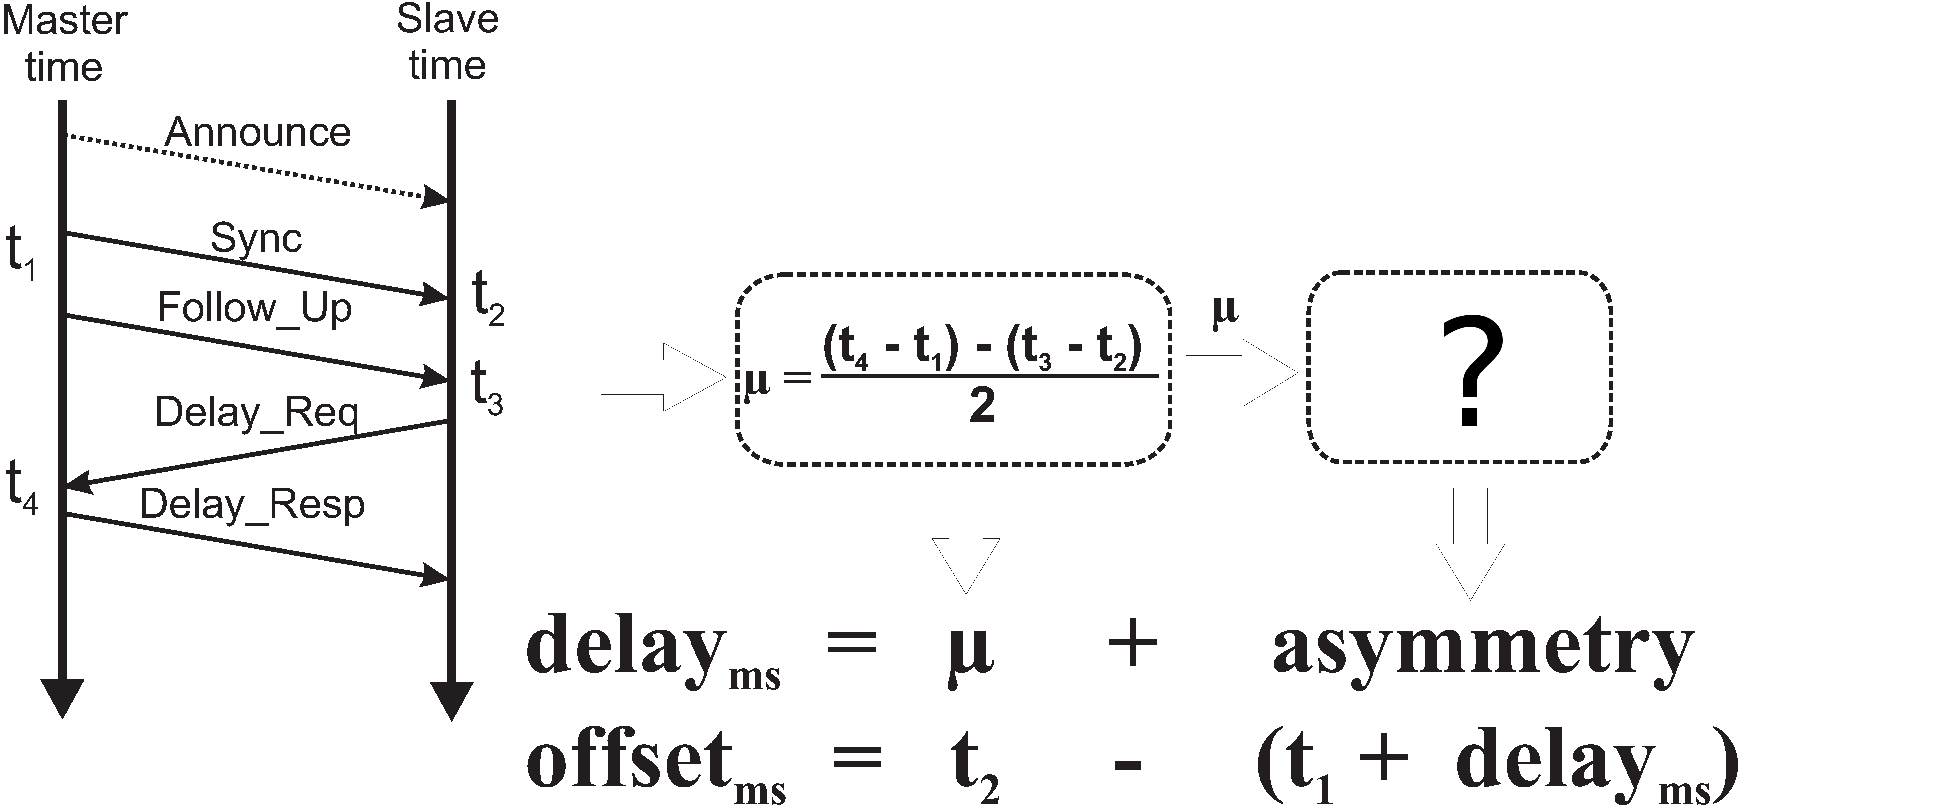
\includegraphics[height=4cm]{../../figures/protocol/wrLinkModel_init.eps}
  \end{center}

\end{frame}
%%%%%%%%%%%%%%%%%%%%%%%%%%%%%%%%%%%%%%%%%%%%%%%%%%%%%%%%%%%%%%%%%%%%%%%%%%%%%%%%%%%%%%%%%%%%%%%%%%%%
% \subsection{}
%%%%%%%%%%%%%%%%%%%%%%%%%%%%%%%%%%%%%%%%%%%%%%%%%%%%%%%%%%%%%%%%%%%%%%%%%%%%%%%%%%%%%%%%%%%%%%%%%%%%
\begin{frame}{Link Delay Model: fiber optic solution}

  \begin{center}
  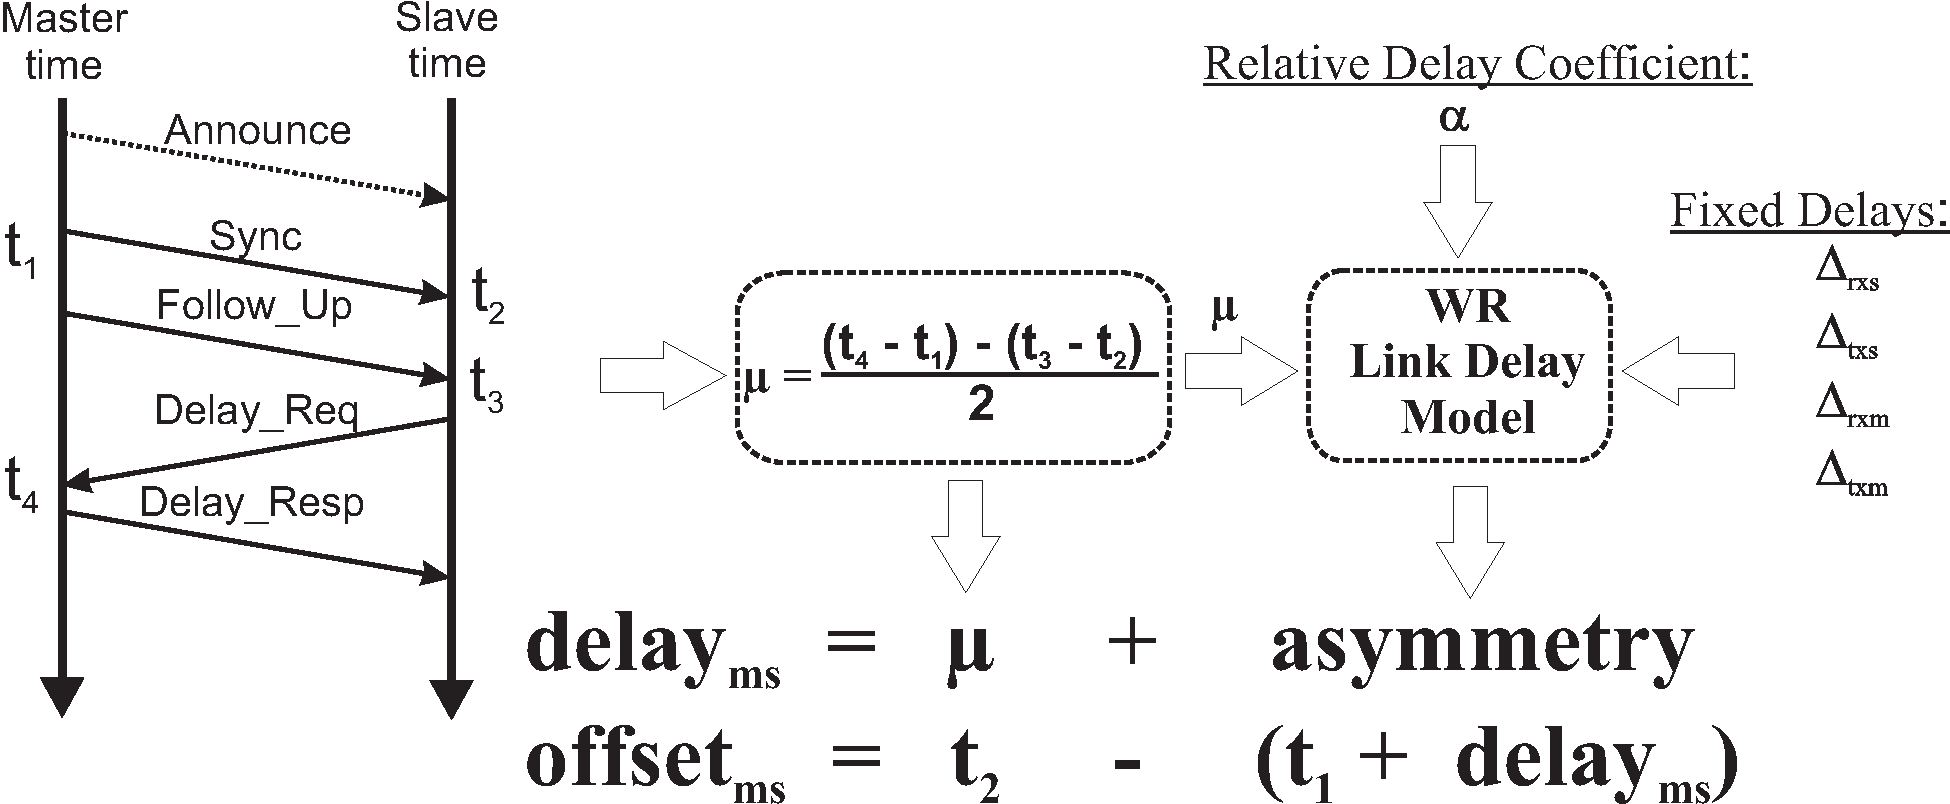
\includegraphics[height=4cm]{../../figures/protocol/wrLinkModel.eps}
  \end{center}

  \begin{columns}[c]
  \column{1.5in}

    \begin{center}
      \textbf{Solution for Ethernet over a Single-mode Optical Fiber}
    \end{center}    

  \column{2.7in}

    \begin{equation}
      \nonumber asymmetry = \Delta_{tx_m} + \Delta_{rx_s} - \frac{\Delta - \alpha \mu + \alpha \Delta}{2 + \alpha}
    \end{equation}

  \end{columns}

\end{frame}
%%%%%%%%%%%%%%%%%%%%%%%%%%%%%%%%%%%%%%%%%%%%%%%%%%%%%%%%%%%%%%%%%%%%%%%%%%%%%%%%%%%%%%%%%%%%%%%%%%%
%\section{PTP\&SyncE}
% \subsection{}
% %%%%%%%%%%%%%%%%%%%%%%%%%%%%%%%%%%%%%%%%%%%%%%%%%%%%%%%%%%%%%%%%%%%%%%%%%%%%%%%%%%%%%%%%%%%%%%%%%%%%
% \begin{frame}{PTP and SyncE in WR}
% 
%   \begin{itemize}
%     \item Compatibility with PTP verified
%     \item Compatibility with SyncE for further study
%     \item Frequency distribution aligned with PTP's logic topology
% %    \item Synchronous Status Message (SSM) mechanism not supported in WR
%     \item PTP's Announce messages used for WR-peers recognition
%   \end{itemize}
% 
% \end{frame}
%%%%%%%%%%%%%%%%%%%%%%%%%%%%%%%%%%%%%%%%%%%%%%%%%%%%%%%%%%%%%%%%%%%%%%%%%%%%%%%%%%%%%%%%%%%%%%%%%%%%
% \section{WRPTP}
% \subsection{}
%%%%%%%%%%%%%%%%%%%%%%%%%%%%%%%%%%%%%%%%%%%%%%%%%%%%%%%%%%%%%%%%%%%%%%%%%%%%%%%%%%%%%%%%%%%%%%%%%%%%
\begin{frame}{White Rabbit extension to PTP (WRPTP)}

  \begin{itemize}
    \item WR-peers recognition
    \item Calibration (fixed delays measurement)
    \item Exchange of WR-data
    \item Support of redundancy
    \item Mapping over IEEE802.3/Ethernet
  \end{itemize}

\end{frame}

%%%%%%%%%%%%%%%%%%%%%%%%%%%%%%%%%%%%%%%%%%%%%%%%%%%%%%%%%%%%%%%%%%%%%%%%%%%%%%%%%%%%%%%%%%%%%%%%%%%%
% \subsection{}
%%%%%%%%%%%%%%%%%%%%%%%%%%%%%%%%%%%%%%%%%%%%%%%%%%%%%%%%%%%%%%%%%%%%%%%%%%%%%%%%%%%%%%%%%%%%%%%%%%%%
\begin{frame}{WR-peer recognition and WR-data exchange}

  \begin{columns}[c]
  \column{.5\textwidth} 

    \begin{center}
    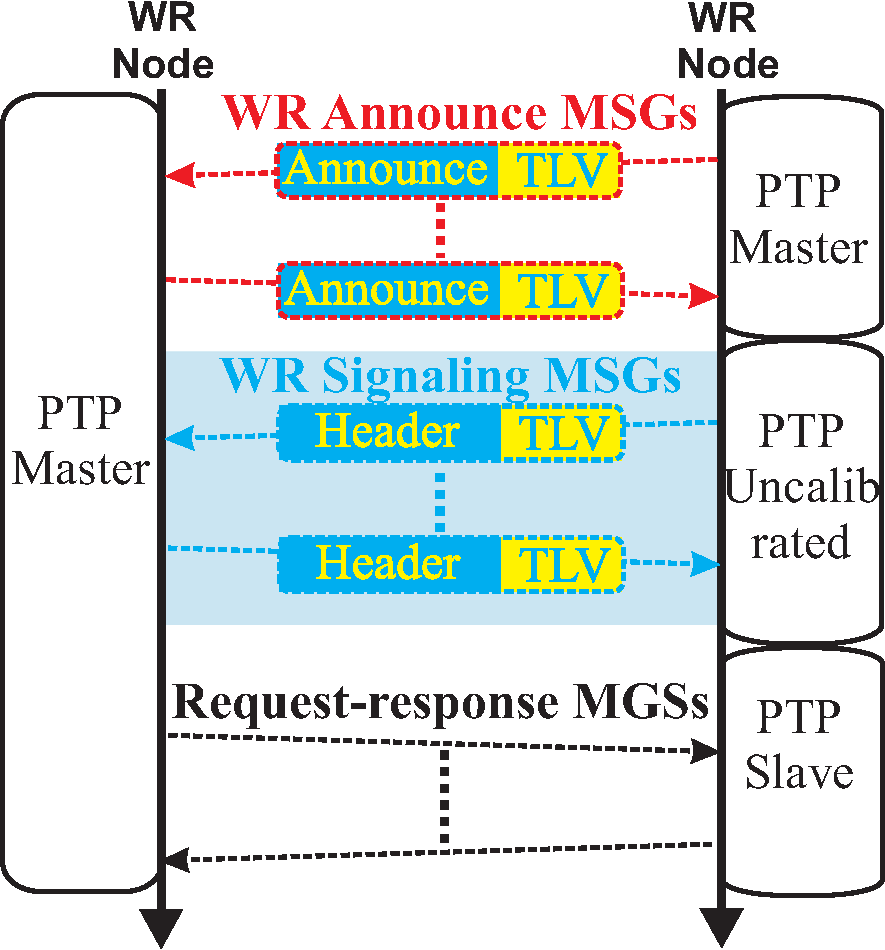
\includegraphics[width=5.0cm]{../../figures/protocol/WR-peer_recognision-1.eps}
    \newline
    Two WR devices
    \end{center}
    
  \column{.5\textwidth}

    \begin{center}
    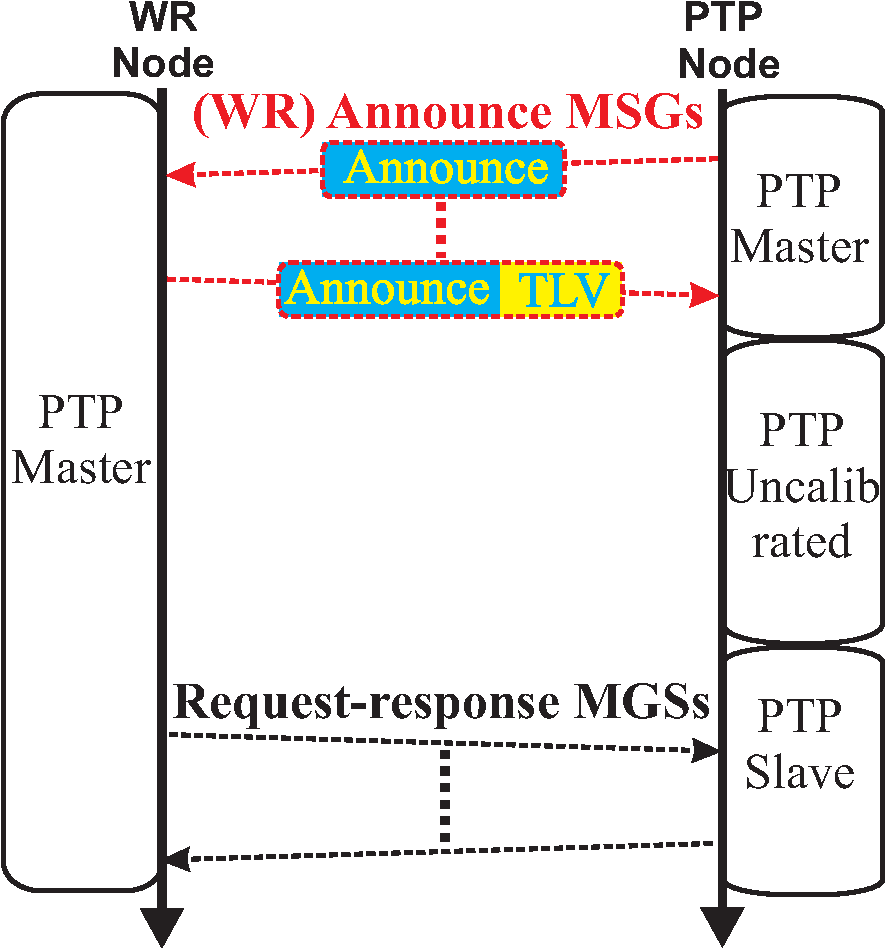
\includegraphics[width=5.0cm]{../../figures/protocol/WR-peer_recognision-2.eps}
    \newline
    WR and non-WR device
    \end{center}
     
  \end{columns}

\end{frame}
%%%%%%%%%%%%%%%%%%%%%%%%%%%%%%%%%%%%%%%%%%%%%%%%%%%%%%%%%%%%%%%%%%%%%%%%%%%%%%%%%%%%%%%%%%%%%%%%%%%%
% \subsection{}
%%%%%%%%%%%%%%%%%%%%%%%%%%%%%%%%%%%%%%%%%%%%%%%%%%%%%%%%%%%%%%%%%%%%%%%%%%%%%%%%%%%%%%%%%%%%%%%%%%%%
\begin{frame}{WR Link Setup }

  \begin{columns}[c]
  \column{.5\textwidth} 

      \begin{center}
      \includegraphics[width=5.5cm]{../../figures/protocol/wrLinkSetup.eps}
      \end{center}


  \column{.5\textwidth} 

      \begin{itemize}
	\item Frequency locking
	\item Calibration
	\item Exchange of WR-parameters
	\item WR Finite State Machine
	\item WR Signaling Messages
      \end{itemize}

  \end{columns}

\end{frame}

%%%%%%%%%%%%%%%%%%%%%%%%%%%%%%%%%%%%%%%%%%%%%%%%%%%%%%%%%%%%%%%%%%%%%%%%%%%%%%%%%%%%%%%%%%%%%%%%%%%%
% \subsection{}
%%%%%%%%%%%%%%%%%%%%%%%%%%%%%%%%%%%%%%%%%%%%%%%%%%%%%%%%%%%%%%%%%%%%%%%%%%%%%%%%%%%%%%%%%%%%%%%%%%%%
% \begin{frame}{Modified Best Master Clock Algorithm (mBMCA)}
% 
%     \begin{center}
%     \includegraphics[height=7.0cm]{../../figures/protocol/mBMCvsBMC.eps}
%     \end{center}
% 
% 
% \end{frame}
%%%%%%%%%%%%%%%%%%%%%%%%%%%%%%%%%%%%%%%%%%%%%%%%%%%%%%%%%%%%%%%%%%%%%%%%%%%%%%%%%%%%%%%%%%%%%%%%%%%%
% \section{H/W for WR}
% \subsection{H/W for WR}
%%%%%%%%%%%%%%%%%%%%%%%%%%%%%%%%%%%%%%%%%%%%%%%%%%%%%%%%%%%%%%%%%%%%%%%%%%%%%%%%%%%%%%%%%%%%%%%%%%%%
% \begin{frame}{Clock Recovery System and mBMCA}
% 
% %{\it [problem with a presentation flow]}
% 
%   \begin{center}
%   \includegraphics[width=11.8cm]{../../figures/protocol/wrCRS+mBMC.eps}
%   \end{center}
% 
% \end{frame}



%%%%%%%%%%%%%%%%%%%%%%%%%%%%%%%%%%%%%%%%%%%%%%%%%%%%%%%%%%%%%%%%%%%%%%%%%%%%%%%%%%%%%%%%%%%%%%%%%%%%
%\section{Status}
%\subsection{}
%%%%%%%%%%%%%%%%%%%%%%%%%%%%%%%%%%%%%%%%%%%%%%%%%%%%%%%%%%%%%%%%%%%%%%%%%%%%%%%%%%%%%%%%%%%%%%%%%%%%
\begin{frame}{WR time transfer performance: temperature tests}

  \begin{columns}[c]
	\column{0.5\textwidth}
		\hspace{-1.0cm}
		\begin{center}
		\includegraphics[width=1.1\textwidth]{../../figures/measurements/tempTests-trends.v3.eps}
		\end{center}

		\begin{center}
		  \begin{table}[!t] \footnotesize 
		  \begin{tabular}{ c  c }     
		  \multicolumn{2}{c}{ }       \\         
		   \multicolumn{2}{c}{ }       \\    
		     &    \\ 
		    &     \\ 
		  \end{tabular}
		  \end{table}   		
		\end{center}

	\column{0.5\textwidth}
		\hspace{-0.8cm}
		\begin{center}
		\includegraphics[width=1.13\textwidth]{../../figures/measurements/tempTests-2-combo.eps}
		\end{center}


  \end{columns} 
\end{frame}



\backupend

%%%%%%%%%%%%%%%%%%%%%%%%%%%%%%%%%%%%%%%%%%%%%%%%%%%%%%%%%%%%%%%%%%%%%%%%%%%%%%%%%%%%%%%%%%%%%%%%%%%%%%%
\end{document}
%%%%%%%%%%%%%%%%%%%%%%%%%%%%%%%%%%%%%%%%%%%%%%%%%%%%%%%%%%%%%%%%%%%%%%%%%%%%%%%%%%%%%%%%%%%%%%%%%%%%%%%